\documentclass[11pt,a4paper]{article}

\usepackage[utf8]{inputenc}
\usepackage[T1]{fontenc}
\usepackage{lmodern}
\usepackage[margin=2.6cm]{geometry}
\usepackage{amsmath,amssymb,amsthm,bm}
\usepackage{enumitem}
\usepackage{booktabs}
\usepackage{xcolor}
\usepackage{tikz}
\usepackage[colorlinks=true,linkcolor=blue!50!black,citecolor=blue!50!black,urlcolor=blue!50!black]{hyperref}
\setlength{\emergencystretch}{2em}

% ---------------------------------------------------------------------------
% Macros (same as hybrid_closure.tex)
% ---------------------------------------------------------------------------
\newcommand{\R}{\mathbb{R}}
\newcommand{\dd}{\,\mathrm{d}}
\newcommand{\tr}{\operatorname{tr}}
\newcommand{\argmin}{\operatorname{arg\,min}}
\newcommand{\argmax}{\operatorname{arg\,max}}
\newcommand{\T}{^{\mathsf T}}
\newcommand{\xh}{\hat{x}}
\newcommand{\eps}{\varepsilon}
\newcommand{\norm}[1]{\left\lVert #1 \right\rVert}
\newcommand{\abs}[1]{\left\lvert #1 \right\rvert}
\newcommand{\grad}{\nabla}
\newcommand{\dt}{\,\delta t}

\theoremstyle{plain}
\newtheorem{proposition}{Proposition}
\newtheorem{lemma}{Lemma}
\theoremstyle{definition}
\newtheorem{definition}{Definition}
\theoremstyle{remark}
\newtheorem{remark}{Remark}

\title{The Mortensen filter in the density representation\\
\large The linear equation for $p=e^{-V/\eps}$, the Gaussian tracker, and the translating window,\\
all derived and solved on the density}
\author{Design note for the \texttt{mortensen} library}
\date{\today}

\begin{document}
\maketitle

\begin{abstract}
This note is a self-contained extract of the hybrid-closure note (\texttt{hybrid\_closure.tex}: its \S1, Appendix~A and Appendix~J.4), rewritten so that \emph{everything is solved on the density} $p=e^{-V/\eps}$. Section~\ref{sec:setting} derives, from the estimation problem, the Hamilton--Jacobi--Bellman equation of the Mortensen filter and its linear form for $p$ --- the equation the four-step cycle of the library discretises; the value function $V$ appears there only to be transformed away. Section~\ref{sec:tracker} inserts a Gaussian ansatz for $p$ into the linear equation and obtains the \emph{tracker} of \texttt{src/tracker.rs} (one state $\xh$, one curvature $S$) by matching orders, then shows that each step of the discrete cycle maps a Gaussian to a Gaussian, which gives the tracker's own cycle without any further approximation. Section~\ref{sec:window} inserts the ansatz $p=\rho(x-\xh(t),t)$ --- a grid density in a \emph{translating} window --- and obtains a closed, exact system for $\rho$ and $\xh$, whose only approximation is the truncation of $\rho$ to a box around the mode; it contains the tracker as the case where $\rho$ is frozen to a Gaussian, and it is the minimal moving-window filter. Section~\ref{sec:rot} lets the window also \emph{rotate}, $\xi=R(t)(x-\xh(t))$ with $R$ orthogonal, keeps the same exact system for $\rho$ and $\xh$, and fixes the rotation by aligning the box with the principal axes of the density at its mode --- which makes a Gaussian separable in the window coordinates, the property Section~\ref{sec:trace} needs. Section~\ref{sec:sum} builds the representation for several competing hypotheses, a sum of Gaussians carried by independent trackers with weights that record the accumulated cost of each hypothesis --- the $\eps$-smoothed form of the min-plus method of McEneaney --- together with the splitting, pruning and merging of the components. Section~\ref{sec:trace} states a low-rank ansatz inside the window, $\rho=\tr\big(G_1(\xi_1)\cdots G_n(\xi_n)\big)$, and the programme --- initialise, diffuse, drift, multiply, compress, read off the mode --- for following the linear equation on its factors. Section~\ref{sec:pop} is the stochastic version of the sum of Section~\ref{sec:sum}, built like the point cloud of \texttt{src/particles.rs}: a population of Gaussians of equal mass, each killed by an exponential clock at the rate of its cost relative to the best, reborn by an exact random split of a survivor, and diffused partly in its width and partly by a random move of its centre --- so that resampling replaces pruning and merging, random splits replace the split tables, and the expectation of the population follows the linear equation.
\end{abstract}

\tableofcontents

% ===========================================================================
\section{The estimation problem and its value function}
\label{sec:setting}
% ===========================================================================

\subsection{Setting}

We observe a dynamical system with state $x(t)\in\R^n$,
\begin{equation}
  \dot x(t) = f\big(x(t)\big) + w(t), \qquad t\in[0,T],
  \label{eq:dyn}
\end{equation}
where $f$ is the known drift and $w(t)\in\R^n$ an unknown \emph{model error}. We record observations
\begin{equation}
  y(t) = h\big(x(t)\big) + v(t),
  \label{eq:obs}
\end{equation}
where $h$ is the known observation operator and $v$ an unknown observation error. No model of any kind is assumed for $w$ or $v$: the Mortensen approach is \emph{deterministic}. Instead we say that a candidate history $(x(\cdot), w(\cdot))$ on $[0,t]$ is \emph{expensive} if it requires large errors, and we measure that expense by the \emph{energy}
\begin{equation}
  J_t\big[x(\cdot), w(\cdot)\big]
  \;=\; V_0\big(x(0)\big)
  \;+\; \frac12\int_0^t \Big( w(s)\T Q^{-1} w(s) \;+\; \gamma\, d\big(y(s), h(x(s))\big)^2 \Big)\dd s .
  \label{eq:energy}
\end{equation}
Here
\begin{itemize}[nosep]
  \item $V_0(x_0)\ge 0$ is the cost of \emph{starting} at $x_0$: it encodes the prior knowledge on the initial state (in the code, $V_0=\sum_d \sigma_d (x_d-x_{c,d})^2/2$, a quadratic prior centred at $x_c$; $\sigma_d=0$ means no prior in direction $d$);
  \item $Q=\operatorname{diag}(q_1,\dots,q_n)\succeq 0$ weights the model error: a large $q_d$ makes it cheap to push the trajectory in direction $d$ (in the code, \texttt{q\_diag});
  \item $d(y,h)$ is the distance in observation space (Euclidean, or the angular distance for a bearing), and $\gamma\ge0$ is the observation weight (\texttt{gamma}): the cost of disagreeing with the data.
\end{itemize}
Only the optimisation structure of \eqref{eq:energy} matters in what follows.

\subsection{The value function}

\begin{definition}[value function]
The \emph{value function} $V(x,t)$ is the smallest energy needed to explain the observations on $[0,t]$ with a trajectory that ends at $x$ at time $t$:
\begin{equation}
  V(x,t) \;=\; \min\Big\{\, J_t[x(\cdot),w(\cdot)] \;:\; \dot x = f(x)+w \text{ on }[0,t],\; x(t)=x \,\Big\}.
  \label{eq:value}
\end{equation}
\end{definition}
The state estimate at time $t$ is the cheapest end point,
\begin{equation}
  \xh(t) = \argmin_x V(x,t),
  \label{eq:estimate}
\end{equation}
the \emph{minimum-energy estimate} of Mortensen~\cite{Mortensen1968} (also Hijab~\cite{Hijab1980}, Krener~\cite{Krener2003}). The whole function $V(\cdot,t)$ is much more than an estimate: its level sets describe how plausible every other state is, and its curvature at the minimum measures the confidence.

\subsection{Dynamic programming: the HJB equation}
\label{sec:hjb}

The key property of $V$ is that it can be updated \emph{recursively} in time, without re-solving the minimisation over the whole past. Consider a small time increment $\delta$ and a trajectory ending at $x$ at time $t+\delta$. Over the last interval $[t,t+\delta]$ it moved with some model error $w$ (constant over the short interval, to first order), so at time $t$ it was at
\[
  x(t) \;=\; x - \delta\,\big(f(x)+w\big) + O(\delta^2),
\]
and paid, during that interval, the running cost $\delta\,\ell(x,w,t)$ with
\[
  \ell(x,w,t) = \tfrac12 w\T Q^{-1}w + \tfrac12\gamma\, d\big(y(t),h(x)\big)^2 .
\]
The cheapest way to reach $x$ at $t+\delta$ is therefore to choose the last error $w$ optimally, having reached $x(t)$ as cheaply as possible before --- and "as cheaply as possible before" is, by definition, $V(x(t),t)$. This is Bellman's principle of optimality:
\begin{equation}
  V(x,t+\delta) \;=\; \min_{w}\Big\{\, V\big(x-\delta(f(x)+w),\,t\big) \;+\; \delta\,\ell(x,w,t) \Big\} + O(\delta^2).
  \label{eq:bellman}
\end{equation}
Now expand to first order in $\delta$, writing $\grad V=\grad_x V(x,t)$:
\[
  V\big(x-\delta(f+w),t\big) = V(x,t) - \delta\,(f+w)\cdot\grad V + O(\delta^2).
\]
Inserting into \eqref{eq:bellman} and dividing by $\delta$,
\begin{equation}
  \partial_t V \;=\; \min_{w}\Big\{ -(f+w)\cdot\grad V + \tfrac12 w\T Q^{-1} w \Big\} + \tfrac12\gamma\, d\big(y,h(x)\big)^2 .
  \label{eq:min_w}
\end{equation}
The minimisation over $w$ is a quadratic problem; its stationarity condition is $-\grad V + Q^{-1}w = 0$, i.e.
\begin{equation}
  w^\star = Q\,\grad V ,
  \label{eq:wstar}
\end{equation}
and the minimal value is
\[
  -f\cdot\grad V - \grad V\T Q\grad V + \tfrac12 \grad V\T Q \grad V = -f\cdot\grad V - \tfrac12\grad V\T Q\grad V .
\]
We have obtained the \textbf{Hamilton--Jacobi--Bellman (HJB) equation} of the Mortensen filter:
\begin{equation}
  \boxed{\;
  \partial_t V + f\cdot\grad V + \tfrac12\,\grad V\T Q\,\grad V \;=\; \tfrac12\gamma\, d\big(y(t),h(x)\big)^2,
  \qquad V(\cdot,0)=V_0 .\;}
  \label{eq:hjb}
\end{equation}
Each term has a clear meaning:
\begin{itemize}[nosep]
  \item $f\cdot\grad V$: the value function is \emph{transported} along the model flow --- a state that is cheap now makes its image under the flow cheap a moment later;
  \item $\tfrac12\grad V\T Q\grad V$: the cost can be \emph{lowered} by spending model error; the optimal error \eqref{eq:wstar} points down the gradient of $V$ with strength $Q$. Note that the optimal trajectories (the \emph{characteristics} of \eqref{eq:hjb}) move with velocity $f + Q\grad V$, not $f$;
  \item the right-hand side is the price of being at $x$ when the current observation is $y(t)$: it \emph{adds} energy where $h(x)$ disagrees with the data.
\end{itemize}

\subsection{The viscous regularisation and the density \texorpdfstring{$p=e^{-V/\eps}$}{p = exp(-V/eps)}}

Equation \eqref{eq:hjb} is a first-order nonlinear PDE; its solutions develop kinks (the minimum over several competing trajectories is not differentiable where they tie), and it must be understood in the viscosity sense~\cite{BardiCD1997}. The standard way to obtain a smooth, well-posed problem is to add a small \emph{viscosity} $\eps>0$:
\begin{equation}
  \partial_t V + f\cdot\grad V + \tfrac12\,\grad V\T Q\,\grad V - \frac{\eps}{2}\tr\big(Q\,\grad^2 V\big) \;=\; \tfrac12\gamma\, d\big(y,h(x)\big)^2 .
  \label{eq:hjb_eps}
\end{equation}
This is the equation the library solves. The value of the regularisation goes far beyond numerics: the \emph{Hopf--Cole transformation}
\begin{equation}
  p(x,t) \;=\; \exp\!\big(-V(x,t)/\eps\big), \qquad V = -\eps\log p,
  \label{eq:hopfcole}
\end{equation}
turns \eqref{eq:hjb_eps} into a \emph{linear} equation. Indeed, with $\grad V=-\eps\grad p/p$ and $\grad^2 V = -\eps\big(\grad^2 p/p - \grad p\grad p\T/p^2\big)$, the two terms in $\grad p\T Q\grad p/p^2$ (one from $\tfrac12\grad V\T Q\grad V$, one from the viscous term) cancel exactly, and multiplying by $-p/\eps$ leaves
\begin{equation}
  \boxed{\;
  \partial_t p \;=\; -\,f\cdot\grad p \;+\; \frac{\eps}{2}\sum_{d=1}^n q_d\,\partial_d^2 p \;-\; \frac{\gamma}{2\eps}\, d\big(y,h(x)\big)^2\, p .\;}
  \label{eq:linear_p}
\end{equation}
This is the equation discretised by the four-step cycle of \texttt{src/filter.rs}: it is an \emph{operator splitting} (Lie splitting, first order in $\dt$) in which each step solves one term of \eqref{eq:linear_p} exactly over one time step:
\begin{center}
\begin{tabular}{@{}lll@{}}
\toprule
step & term of \eqref{eq:linear_p} & exact solution over $\dt$ \\
\midrule
1. observation & $-\frac{\gamma}{2\eps} d^2\, p$ & $p \leftarrow p\cdot\exp\!\big(-\eps^{-1}\dt\,\gamma\, d^2/2\big)$ \\
2--3. transport & $-f\cdot\grad p$ & $p(x) \leftarrow p\big(\varphi^{-1}(x)\big)$, $\varphi$ the flow of $\dot x=f(x)$ over $\dt$ \\
4. diffusion & $\frac{\eps}{2}\sum_d q_d\partial_d^2 p$ & one implicit-Euler step of the anisotropic heat equation \\
\bottomrule
\end{tabular}
\end{center}
Step 2 (advancing the reference trajectory) only refreshes the observation $y$. Note that the transport is $p(x)\leftarrow p(\varphi^{-1}(x))$ and \emph{not} a conservative transport (there is no $-(\grad\!\cdot\! f)\,p$ term): $p$ is the exponential of a value function, transported like $V$, and its overall scale has no meaning --- only its shape, its maximiser $\xh=\argmax p=\argmin V$ and its curvature there matter. From here on \emph{every object is a density}: the two reduced filters of \S\ref{sec:tracker} and \S\ref{sec:window} are obtained by inserting an ansatz for $p$ into \eqref{eq:linear_p} --- never into \eqref{eq:hjb_eps} --- and each step of their discrete cycles is an operation on a density.


\subsection{Refinements (may be skipped on first reading)}
\label{sec:refinements}

\emph{The two paragraphs below answer questions a careful reader will ask --- where the viscous term of \eqref{eq:hjb_eps} comes from, and what the boundary conditions of the discretisation mean --- but nothing in the rest of the note depends on them. Everything stays deterministic: the viscous term is a \emph{soft minimum}.}

\subsubsection{Where the viscous term comes from: the soft minimum}
\label{sec:softmin}

Can \eqref{eq:hjb_eps} be obtained, like \eqref{eq:hjb}, as the dynamic-programming equation of some energy? Not with a pointwise minimum: in the derivation of \S\ref{sec:hjb} the state moves by $O(\delta)$ over a time $\delta$, so the expansion of $V(x-\delta(f+w),t)$ stops at first order in $\grad V$ whatever the running cost, and one always obtains a first-order equation $\partial_tV + \mathcal H(x,\grad V)=\text{source}$. The viscous term comes from replacing the \emph{minimum} over the model error by a \emph{soft minimum}. This is best seen on one step of the discrete cycle. One deterministic step is an \emph{inf-convolution} (Hopf--Lax formula):
\[
  V^+(x) = \min_w\Big\{V\big(x-\delta f-\delta w\big) + \delta\,\tfrac12 w\T Q^{-1}w\Big\}.
\]
Replace the minimum over $w$ by the soft minimum of temperature $\eps$, $\min_w a(w)\ \to\ -\eps\log\int e^{-a(w)/\eps}\dd w$ (a log-sum-exp, which tends to the minimum as $\eps\to0$ by Laplace's method). Then
\[
  e^{-V^+(x)/\eps} = \int e^{-V(x-\delta f-\delta w)/\eps}\, e^{-\delta\, w\T Q^{-1}w/(2\eps)}\dd w
  \;\propto\; \big(p\circ\text{shift by }\delta f\big) * G_{\eps\delta Q},
\]
with $G_\Sigma(\xi) := e^{-\xi\T\Sigma^{-1}\xi/2}$: a convolution with the Gaussian function $G_{\eps\delta Q}$ --- precisely the heat kernel of the diffusion $\tfrac{\eps}{2}\sum_d q_d\partial_d^2$ over time $\delta$, i.e.\ the diffusion step of the library. The transport and diffusion steps are thus the soft-min version of "transport, then optimise the model error"; the diffusion step is where the minimum over $w$ became an integral. Iterating over the steps, the value function of \eqref{eq:hjb_eps} is the soft minimum of the energy over all histories,
\begin{center}
  deterministic Mortensen: $V=\displaystyle\min_{\text{paths}} J_t$, \qquad
  viscous Mortensen: $V = -\eps\log\displaystyle\int_{\text{paths}} e^{-J_t/\eps}$,
\end{center}
with the same energy \eqref{eq:energy}: the regularisation does not change what is measured, only how the minimum is taken. In the limit $\eps\to0$ the soft minimum becomes the minimum and \eqref{eq:hjb_eps} becomes \eqref{eq:hjb}, which is why $\eps$ is called the temperature.

\begin{remark}[the soft minimum as a minimum: relaxed choices with an entropy price]
\label{rem:gibbs}
The viscous equation \eqref{eq:hjb_eps} can be obtained from a modification of the definition \eqref{eq:value} that stays deterministic. The identity behind the soft minimum is variational: for any function $a$,
\begin{equation}
  -\eps\log\int e^{-a(w)/\eps}\dd w \;=\; \min_{\pi\ge0,\ \int\pi=1}\ \Big\{\int a(w)\,\pi(w)\dd w \;+\; \eps\int\pi\log\pi\dd w\Big\},
  \label{eq:gibbs}
\end{equation}
the minimum being attained at $\pi\propto e^{-a/\eps}$ (Jensen's inequality). Applied to one step with $a(w)=V(x-\delta f-\delta w)+\delta\,\tfrac12w\T Q^{-1}w$, it says that the soft-min step is the \emph{minimum} over \emph{relaxed} model errors: the controller chooses a spread $\pi$ of errors rather than one error, pays the average of the running cost under $\pi$, and pays in addition $\eps$ times the negative entropy of the spread. So \eqref{eq:hjb_eps} is the dynamic-programming equation of \eqref{eq:value} with the minimum over histories $w(\cdot)$ replaced by a minimum over relaxed histories --- distributions of $w$ at each instant, a standard object of deterministic control theory --- and the energy \eqref{eq:energy} augmented by the entropy of the relaxation, weighted by $\eps$; the sharp choice is the limit $\eps\to0$. In continuous time the entropy must be taken relative to a reference on paths whose construction is the one place where a stochastic object appears; in the time-discrete cycle the reference is Lebesgue measure per step and \eqref{eq:gibbs} is elementary. A second deterministic route, not used here, is the two-person game of Kohn and Serfaty (Comm.\ Pure Appl.\ Math., 2006 and 2010): a controller choosing a direction and an adversary the sign of a move of size $\sqrt{2\eps\,\delta}$, whose value converges to the viscosity solution of the second-order equation. What cannot work is a minimum over single paths with increments $O(\delta)$, which always gives a first-order equation.
\end{remark}

\subsubsection{Boundary conditions as state constraints}
\label{sec:bc}

The grid filter works on a box $\Omega$ and needs boundary conditions on $\partial\Omega$: Neumann $\partial_n p=0$ by default, periodic for angles, and optionally homogeneous Dirichlet $p=0$, i.e.\ $V=+\infty$ on the wall (\texttt{FilterParams::dirichlet}). The Dirichlet condition has an exact justification in the framework of \S\ref{sec:softmin}: it is the value function of the \emph{state-constrained} problem "the trajectory must stay in $\Omega$", the constraint being enforced as an infinite cost. Modify the energy by an indicator penalty,
\[
  J_t^{\Omega} = J_t + \int_0^t \chi_\Omega\big(x(s)\big)\dd s, \qquad \chi_\Omega = 0 \text{ in }\Omega,\ +\infty\text{ outside},
\]
so that every path leaving the box costs $+\infty$ --- this is the semantics implemented in the code, \emph{$p\equiv0$ outside the box}. In the soft-min form of \S\ref{sec:softmin}, $e^{-\int\chi_\Omega/\eps}$ is the indicator that the history stayed in $\Omega$: the integral over the model error in the inf-convolution step is restricted to the displacements that stay inside, which turns the free-space heat kernel $G_{\eps\delta Q}$ into the heat kernel of $\Omega$ with $p=0$ on $\partial\Omega$. In one line: \emph{Dirichlet $=$ infinite cost outside $=$ $p\equiv0$ outside.} By contrast, Neumann is the heat kernel of $\Omega$ with reflection at the wall: a history that reaches the wall is pushed back inside at no cost, a frictionless barrier the state may slide along. Both are state constraints; they differ in whether touching the wall is allowed.

\paragraph{The deterministic limit.}
At $\eps=0$ the constrained problem has a value function that is finite up to the boundary (one may end on the wall while staying inside), and the correct boundary condition is Soner's constrained viscosity-solution condition~\cite{Soner1986}, not $V=+\infty$. The two pictures are reconciled by a boundary layer: the Dirichlet heat kernel vanishes linearly at the wall, so near it $p$ behaves like $\operatorname{dist}(x,\partial\Omega)/\sqrt{\eps q t}$ times its interior value ($q$ the noise weight $q_d$ of the direction normal to the wall), and
\[
  V_\eps(x) \approx V_{\eps=0}(x) - \eps\log\frac{\operatorname{dist}(x,\partial\Omega)}{\sqrt{\eps q t}},
\]
(with $V_{\eps=0}$ the constrained deterministic value function, not the prior $V_0$) --- a logarithmic layer of width $\sim\sqrt{\eps q t}$ that disappears as $\eps\to0$ at every interior point. Dirichlet is therefore the consistent $\eps$-regularisation of the state-constrained Mortensen problem; numerically, the layer is the sag of $p$ near the wall over a decay length $\sqrt{\dt\,\eps q/2}$ per step (test \texttt{dirichlet\_diffusion\_absorbs\_at\_the\_boundary}).

\paragraph{Two consequences for the discretisation.}
The Dirichlet heat kernel on a half-space is, by the method of images, $G(x-y)-G(x-\bar y)$ with $\bar y$ the mirror point: the \emph{odd extension}. The sine basis of the Dirichlet diffusion solver is therefore exactly this kernel. But the odd extension is a device for the \emph{diffusion} kernel only: in the transport step, a grid point whose preimage $\varphi^{-1}(x)$ lies outside the box corresponds to a history that was outside, hence of infinite cost, so it must receive $p=0$, not the odd extension's $-p(\text{mirror})$. This is what the code does (test \texttt{dirichlet\_transport\_zeroes\_outside\_preimages}).

\paragraph{Modelling content, and a soft wall.}
Dirichlet asserts prior knowledge: the state cannot leave $\Omega$, and cannot even approach the wall closer than the layer width without penalty. Neumann asserts nothing about the state and is the pragmatic choice when the box is a mere computational truncation, since it creates no layer; if the box is large enough for $p$ to be negligible at the wall, the two agree. A smooth intermediate is the penalised constraint $\chi_\Omega \to \tfrac12\kappa\operatorname{dist}(x,\Omega)^2$ on an enlarged box: in the code this is one extra multiplicative factor $\exp(-\dt\,\kappa\operatorname{dist}^2/(2\eps))$ in the observation step, converging to Dirichlet as $\kappa\to\infty$ --- a tunable confinement without unstored boundary nodes, possibly a useful third option.

% ===========================================================================
\section{The Gaussian closure on the density: the tracker}
% ===========================================================================
\label{sec:tracker}

Solving \eqref{eq:linear_p} on a grid with $N_d$ nodes in direction $d$ costs $\prod_dN_d$ degrees of freedom, exponential in $n$. The oldest way to make it tractable is to \emph{assume a shape} for $p$ and keep only the parameters of that shape. The tracker of \texttt{src/tracker.rs} assumes that $p$ is a Gaussian:
\begin{equation}
  p(x,t) \;\approx\; a(t)\,\exp\Big(-\frac{1}{2\eps}\,\xi\T S(t)\,\xi\Big), \qquad \xi := x-\xh(t),
  \label{eq:ansatz_tracker}
\end{equation}
i.e.\ a mode at $\xh(t)\in\R^n$, a width matrix $\eps\,S(t)^{-1}$ with $S=S\T\succ0$ the \emph{information} (the curvature of $V=-\eps\log p$ at the mode), and a height $a(t)>0$ that carries no information (recall that $p$ is unnormalised). To obtain the evolution of $(a,\xh,S)$, insert \eqref{eq:ansatz_tracker} into the linear equation \eqref{eq:linear_p} and expand in powers of $\xi$; the ansatz has three parameters (a scalar, a vector, a matrix), so only the orders $0,1,2$ can be matched, and all higher orders are dropped. This is the \emph{second-order closure}.

\subsection{Inserting the ansatz into the linear equation}

We need $f$ and $h$ near $\xh$: linearise, $f(x)\approx f(\xh)+F\xi$ with $F=\partial f(\xh)$, and $h(x)\approx h(\xh)+H\xi$ with $H=\partial h(\xh)$, so that
\[
  d\big(y,h(x)\big)^2 \approx \abs{r - H\xi}^2, \qquad r := y \ominus h(\xh),
\]
is the \emph{innovation} (signed difference in the observation's own geometry --- plain difference, or shortest angle for a bearing). The derivatives of the Gaussian \eqref{eq:ansatz_tracker} are all multiples of $p$ by polynomials in $\xi$:
\begin{equation}
  \partial_tp = \Big[\frac{\dot a}{a} + \frac1\eps\,\dot{\xh}\T S\xi - \frac{1}{2\eps}\,\xi\T\dot S\xi\Big]p, \qquad
  \grad p = -\frac1\eps\,S\xi\,p, \qquad
  \grad^2p = \Big[-\frac1\eps\,S + \frac1{\eps^2}\,S\xi\xi\T S\Big]p ,
  \label{eq:gauss_derivs}
\end{equation}
where $\partial_tp$ uses $\partial_t\xi = -\dot{\xh}$. Hence $\tr(Q\grad^2p) = \big[-\tfrac1\eps\tr(QS) + \tfrac1{\eps^2}\,\xi\T SQS\xi\big]p$. Insert into \eqref{eq:linear_p} and divide by $p$ (which never vanishes): the equation becomes a polynomial identity in $\xi$,
\begin{equation}
  \frac{\dot a}{a} + \frac1\eps\,\dot{\xh}\T S\xi - \frac{1}{2\eps}\,\xi\T\dot S\xi
  \;=\; \frac1\eps\,\big(f(\xh)+F\xi\big)\T S\xi \;-\; \frac12\tr(QS) + \frac{1}{2\eps}\,\xi\T SQS\xi \;-\; \frac{\gamma}{2\eps}\,\abs{r-H\xi}^2 .
  \label{eq:tracker_inserted}
\end{equation}
Sort by order in $\xi$ (multiplying by $\eps$ for readability):
\begin{align*}
  \text{order }0:&\quad \eps\,\frac{\dot a}{a} = -\frac\eps2\tr(QS) - \tfrac12\gamma\abs r^2 ,\\
  \text{order }1:&\quad \dot{\xh}\T S\xi = f(\xh)\T S\xi + \gamma\,r\T H\xi ,\\
  \text{order }2:&\quad -\tfrac12\,\xi\T\dot S\xi = \xi\T F\T S\xi + \tfrac12\,\xi\T SQS\xi - \tfrac12\gamma\,\xi\T H\T H\xi .
\end{align*}
The order-1 identity must hold for every $\xi$, hence (using $S=S\T$)
\begin{equation}
  \boxed{\;\dot{\xh} \;=\; f(\xh) + \gamma\, S^{-1}H\T r ,\;}
  \label{eq:tracker_x}
\end{equation}
and the order-2 identity, after symmetrising $\xi\T F\T S\xi = \tfrac12\xi\T(F\T S+SF)\xi$,
\begin{equation}
  \boxed{\;\dot S \;=\; \gamma\,H\T H - F\T S - S F - S Q S .\;}
  \label{eq:tracker_S}
\end{equation}
The order-0 identity gives the decay of the height, $\dot a/a = -\tfrac12\tr(QS) - \tfrac{\gamma}{2\eps}\abs r^2$: the observation lowers $p$ everywhere by the misfit at the mode, and the diffusion lowers the peak of a Gaussian that widens. Three observations:
\begin{itemize}[nosep]
  \item $\eps$ has disappeared from \eqref{eq:tracker_x}--\eqref{eq:tracker_S}: in \eqref{eq:tracker_inserted} every term of order $1$ and $2$ carries the same factor $1/\eps$, from $\grad p$ and from the $\xi\xi\T$ part of $\grad^2p$, and only the $\xi$-free part of the diffusion, $-\tfrac1\eps\tr(QS)$, comes with a different power --- it goes to the height $a$, which is irrelevant to the estimate and its curvature. The tracker is the $\eps\to0$ limit of the closure, Mortensen's second-order minimum-energy estimator~\cite{Mortensen1968}.
  \item In terms of $P=S^{-1}$, \eqref{eq:tracker_S} reads $\dot P = FP + PF\T + Q - \gamma\,PH\T HP$: the Riccati equation of the (extended) Kalman filter with observation weight $\gamma$, recovered here as a purely deterministic least-squares estimator. When $f$ and $h$ are affine and $p_0$ Gaussian, the ansatz \eqref{eq:ansatz_tracker} is \emph{exact} (each term of \eqref{eq:linear_p} maps a Gaussian to a Gaussian times a polynomial of degree $\le2$, see \S\ref{sec:tracker_cycle}) and the tracker \emph{is} the Kalman filter --- this is the test \texttt{matches\_kalman\_filter\_on\_linear\_model}.
  \item The width of the density $p$ is $\eps P$, not $P$: an uncertainty band drawn from the tracker must be $\pm2\sqrt{\eps P_{dd}}$ (the viewer's \texttt{tracker\_view}).
\end{itemize}
The closure is unimodal by construction: it cannot represent a density with two competing maxima, and when the true $p$ has them (e.g.\ a phase-aliased misfit, as for the unknown-$\mu$ Kepler problem) the tracker follows one of them, not necessarily the right one.

\subsection{The discrete cycle: every step maps a Gaussian to a Gaussian}
\label{sec:tracker_cycle}

The library does not integrate \eqref{eq:tracker_x}--\eqref{eq:tracker_S} as ODEs: it applies the same four-step splitting as the grid filter to the Gaussian \eqref{eq:ansatz_tracker}, and each step is \emph{exact} on Gaussians once $f$ and $h$ are linearised. This is the content of \texttt{MortensenTracker::forward}.

\paragraph{Step 1 --- observation.}
Multiplying \eqref{eq:ansatz_tracker} by $\exp\big(-\eps^{-1}\dt\,\gamma\abs{r-H\xi}^2/2\big)$ multiplies two Gaussians in $\xi$; the exponent $-\tfrac1{2\eps}\big[\xi\T S\xi + \dt\,\gamma\abs{r-H\xi}^2\big]$ is again quadratic. Completing the square,
\begin{equation}
\begin{gathered}
  S^+ = S + \dt\,\gamma\,H\T H, \qquad
  \xh^+ = \xh + \dt\,\gamma\,(S^+)^{-1}H\T r, \\
  a^+ = a\,\exp\Big(-\frac{\dt\,\gamma}{2\eps}\Big[\abs r^2 - \dt\,\gamma\, r\T H(S^+)^{-1}H\T r\Big]\Big),
\end{gathered}
  \label{eq:cycle_obs}
\end{equation}
where the shift of the mode is read off the stationarity of the new exponent, $S\xi - \dt\,\gamma H\T(r-H\xi) = 0$. Note the \emph{updated} $S^+$ in the mean update (the code: \texttt{s += dt*gamma*H\textasciicircum T*H} first, then \texttt{x\_hat += dt*gamma*solve(s, H\textasciicircum T*r)}): this is the exact product of the two Gaussians, not a first-order approximation of \eqref{eq:tracker_x}. Cost: one $n\times n$ solve.

\paragraph{Steps 2--3 --- transport.}
The transport is $p^+(x) = p\big(\varphi^{-1}(x)\big)$ with $\varphi$ the discrete flow over $\dt$. Linearise $\varphi$ at $\xh$: $\varphi^{-1}(x) \approx \xh + \Phi^{-1}\big(x - \varphi(\xh)\big)$ with $\Phi = \partial\varphi(\xh)$ the exact tangent of the discrete step (\texttt{gl4\_step\_with\_jacobian}). Then $p^+(x) = a\exp\big(-\tfrac1{2\eps}\,\xi^{+\mathsf T}\Phi^{-\mathsf T}S\Phi^{-1}\xi^+\big)$ with $\xi^+ = x-\varphi(\xh)$:
\begin{equation}
  \xh^+ = \varphi(\xh), \qquad S^+ = \Phi^{-\mathsf T}\,S\,\Phi^{-1}, \qquad a^+ = a .
  \label{eq:cycle_transport}
\end{equation}
Exact when $\varphi$ is affine; the height is unchanged because the transport of \eqref{eq:linear_p} is the non-conservative $p\circ\varphi^{-1}$ (a conservative transport would also pick up $\det\Phi^{-1}$).

\paragraph{Step 4 --- diffusion.}
The heat flow $\partial_\tau p = \tfrac\eps2\sum_dq_d\partial_d^2p$ over a time $\dt$ is the convolution with the Gaussian function $G_{\eps\dt Q}$ of \S\ref{sec:softmin}, and the convolution of two Gaussians is a Gaussian whose width matrices add: $\eps S^{-1} \to \eps\,(S^{-1} + \dt\,Q)$, i.e.
\begin{equation}
  S^+ = \big(S^{-1} + \dt\,Q\big)^{-1} = S\,(I + \dt\,QS)^{-1}, \qquad \xh^+ = \xh, \qquad a^+ = a\,\det(I+\dt\,QS)^{-1/2}.
  \label{eq:cycle_diff}
\end{equation}
This is the \emph{exact} semigroup on Gaussians; the code applies the form $S(I+\dt\,QS)^{-1}$, which needs no inversion of $S$ (and so tolerates a flat prior, $S$ singular). The grid filter, by contrast, applies one implicit-Euler step of the same heat flow; the two agree to $O(\dt^2)$, and the tracker's step is the one that is exact.

\paragraph{Summary.}
\begin{center}\small
\begin{tabular}{@{}llll@{}}
\toprule
step & operation on $p$ & $\xh$ & $S$ \\
\midrule
observation & product of Gaussians & $\xh + \dt\gamma(S^+)^{-1}H\T r$ & $S+\dt\gamma H\T H$ \\
model forward & refresh $y$, $r$, $H$ & --- & --- \\
transport & $p\circ\varphi^{-1}$, $\varphi$ linearised & $\varphi(\xh)$ & $\Phi^{-\mathsf T}S\Phi^{-1}$ \\
diffusion & Gaussian convolution & --- & $S(I+\dt\,QS)^{-1}$ \\
\bottomrule
\end{tabular}
\end{center}
Everything is an operation on the density; the only approximations are the linearisations of $h$ (step 1) and $\varphi$ (step 3) at the mode --- absent for a linear model, where the cycle reproduces the discrete Kalman filter to round-off.

% ===========================================================================
\section{The translating window: \texorpdfstring{$p=\rho(x-\xh(t),t)$}{p = rho(x - xhat(t), t)}}
% ===========================================================================
\label{sec:window}

The grid filter pays for its generality with a box that must contain every state the reference may visit, resolved uniformly; the tracker pays for its cheapness with a single Gaussian. Between the two sits a grid that \emph{follows the mode}: a small box around $\xh(t)$ on which $p$ is represented without any assumption on its shape. The simplest version keeps the axes of the original coordinates and only lets the grid translate:
\begin{equation}
  p(x,t) \;=\; \rho\big(\xi,t\big), \qquad \xi := x-\xh(t),
  \label{eq:tr_ansatz}
\end{equation}
with $\rho$ a function on a grid in $\xi$ and $\xh(t)$ the position of that grid. Unlike \eqref{eq:ansatz_tracker}, \eqref{eq:tr_ansatz} is \emph{not} a closure: with $\rho$ arbitrary it is a change of variables, exact for \emph{any} $\xh(t)$, and the choice of $\xh$ is a gauge. It becomes an approximation only when $\rho$ is restricted to a box $\abs{\xi_d}\le L_d$ with $p\equiv0$ outside (the Dirichlet-wall semantics of \S\ref{sec:bc}). The gauge must therefore be fixed so that the truncation is harmless, i.e.\ so that the grid stays centred on the mode; the analysis below does this and yields a closed system for $\rho$ and $\xh$ in which every equation is an equation on the density. (The rotating window, $\xi=R(t)(x-\xh(t))$ with $R$ orthogonal, is \S\ref{sec:rot}; the general frame, where $R$ also scales the grid, is analysed in Appendix~J of the hybrid-closure note; the translating case is the one to implement first.)

\subsection{The equation in the moving frame}

\begin{lemma}
Under \eqref{eq:tr_ansatz}, $p$ solves \eqref{eq:linear_p} if and only if $\rho$ solves
\begin{equation}
  \boxed{\;
  \partial_t\rho \;+\; \big(f(\xh+\xi) - \dot{\xh}\big)\cdot\grad\rho
  \;=\; \frac\eps2\sum_{d=1}^nq_d\,\partial_d^2\rho \;-\; \frac{\gamma}{2\eps}\,d\big(y,h(\xh+\xi)\big)^2\,\rho ,\;}
  \label{eq:tr_rho}
\end{equation}
all derivatives being in $\xi$.
\end{lemma}
\begin{proof}
At fixed $x$, $\partial_t\xi = -\dot{\xh}$, so $\partial_tp = \partial_t\rho - \dot{\xh}\cdot\grad\rho$, while $\grad_xp = \grad_\xi\rho$ and $\grad^2_xp = \grad^2_\xi\rho$. Substitute in \eqref{eq:linear_p} with $x = \xh+\xi$.
\end{proof}

Equation \eqref{eq:tr_rho} is the linear equation seen from a frame moving at the velocity $\dot{\xh}$: the flow and the observation are evaluated at $\xh+\xi$, the drift gains the term $-\dot{\xh}$, and the diffusion is unchanged --- diagonal, so the current solver applies verbatim. The four-step cycle applies to \eqref{eq:tr_rho} as it applies to \eqref{eq:linear_p}.

\subsection{The gauge, and the equation for \texorpdfstring{$\xh$}{xhat}}

The condition that fixes the frame is that the mode of $\rho$ be the origin of the grid,
\begin{equation}
  \grad\rho(0,t) \;=\; 0 \qquad\text{for all } t,
  \label{eq:tr_gauge}
\end{equation}
i.e.\ $\xh(t) = \argmax_xp(\cdot,t)$; we assume the mode nondegenerate, $-\grad^2\rho(0,t)\succ0$. It closes the system: \eqref{eq:tr_gauge} determines $\dot{\xh}$ from $\rho$, and \eqref{eq:tr_rho} then evolves $\rho$.

\begin{proposition}[translating window]
\label{prop:tr}
Let $\rho$ solve \eqref{eq:tr_rho}. The gauge \eqref{eq:tr_gauge} holds for all $t$ if and only if it holds at $t=0$ and
\begin{equation}
  \boxed{\;
  \dot{\xh} \;=\; f(\xh) \;+\; \frac{\gamma}{\eps}\,C^{-1}H\T r \;+\; \frac\eps2\,C^{-1}\,\frac{\big(Q\!:\!\grad^3\rho\big)(0,t)}{\rho(0,t)},
  \qquad C := -\,\frac{\grad^2\rho(0,t)}{\rho(0,t)} \succ 0,\;}
  \label{eq:tr_xhat}
\end{equation}
where $r = y\ominus h(\xh)$, $H=\partial h(\xh)$, and $(Q\!:\!\grad^3\rho)_c = \sum_{a,b}Q_{ab}\,\partial_{abc}\rho$ --- for diagonal $Q$, $\sum_aq_a\,\partial_{aac}\rho$. The system \eqref{eq:tr_rho}, \eqref{eq:tr_xhat} is exact: it is \eqref{eq:linear_p} in a moving frame, no approximation being made until $\rho$ is truncated to a box in $\xi$.
\end{proposition}
\begin{proof}
Differentiate \eqref{eq:tr_gauge} in time: $\partial_t\grad\rho(0,t)=0$. Take the gradient of \eqref{eq:tr_rho} at $\xi=0$, where $\grad\rho=0$. The drift term gives $\grad\big[(f(\xh+\xi)-\dot{\xh})\cdot\grad\rho\big]_{\xi=0} = F\T\grad\rho(0) + \grad^2\rho(0)\,\big(f(\xh)-\dot{\xh}\big) = \grad^2\rho(0)\,\big(f(\xh)-\dot{\xh}\big)$, with $F=\partial f(\xh)$; the diffusion gives $\tfrac\eps2\,(Q\!:\!\grad^3\rho)(0)$; the misfit gives $-\tfrac{\gamma}{2\eps}\big[\rho(0)\,\grad(d^2)(0) + d^2\,\grad\rho(0)\big] = \tfrac\gamma\eps\,\rho(0)\,H\T r$, since $\grad_\xi\,d\big(y,h(\xh+\xi)\big)^2\big|_{\xi=0} = -2H\T r$. Hence
\[
  0 = \partial_t\grad\rho(0) = -\grad^2\rho(0)\big(f(\xh)-\dot{\xh}\big) + \tfrac\eps2\,(Q\!:\!\grad^3\rho)(0) + \tfrac\gamma\eps\,\rho(0)\,H\T r ,
\]
and solving for $\dot{\xh}$ with $\grad^2\rho(0) = -\rho(0)\,C$ gives \eqref{eq:tr_xhat}. Conversely, if \eqref{eq:tr_xhat} holds then $\partial_t\grad\rho(0,t)=0$, so $\grad\rho(0,t)=\grad\rho(0,0)=0$.
\end{proof}

\subsection{Reading the equation for \texorpdfstring{$\xh$}{xhat}}

Three terms move the window:
\begin{itemize}[leftmargin=1.5em]
  \item $f(\xh)$: the frame follows the flow --- the transport of the mode;
  \item $\tfrac\gamma\eps C^{-1}H\T r$: the observation pulls the mode toward the data by the innovation, weighted by the inverse curvature of $\rho$. With $S := \eps\,C$ --- the curvature of $-\eps\log\rho$ at the mode, i.e.\ the tracker's information --- this is exactly the tracker's gain $\gamma S^{-1}H\T r$ of \eqref{eq:tracker_x}. It looks $O(\eps^{-1})$ in $\rho$-units because $C$, the curvature of $\rho$ itself, is $O(\eps^{-1})$ where $p$ is sharp; the product is $O(1)$;
  \item $\tfrac\eps2C^{-1}(Q\!:\!\grad^3\rho)/\rho$: the diffusion moves the mode toward the heavy tail when $\rho$ is skewed. In one dimension, $\rho\propto e^{-(\sigma\xi^2/2 + a\xi^3/6)/\eps}$ with $a>0$ is steeper on the right, so its heavy tail is on the left; $\partial^3\rho(0)/\rho(0) = -a/\eps$ and the term is $-\eps qa/(2\sigma)<0$: the mode moves left, as it must. It vanishes when $\rho$ is Gaussian at the origin ($\grad^3\rho(0)=0$).
\end{itemize}

\begin{remark}[the tracker as a frozen window]
Freeze $\rho$ to the Gaussian \eqref{eq:ansatz_tracker}: $C = S/\eps$, $\grad^3\rho(0)=0$, and \eqref{eq:tr_xhat} is \eqref{eq:tracker_x}. The tracker is the translating window whose density is not allowed to change shape; its second equation \eqref{eq:tracker_S} is what \eqref{eq:tr_rho} does to the curvature of $\rho$ when $\rho$ is Gaussian. In the window, $S=\eps C$ is not an unknown but a \emph{diagnostic} read off $\rho$ at the origin, and its evolution --- including the terms the tracker drops: the second derivative of $h$, the third and fourth derivatives of $-\eps\log\rho$ --- is produced by \eqref{eq:tr_rho} automatically. The estimate is $\xh$ and the uncertainty is $\rho$ itself; the tracker's $\pm2\sqrt{\eps P}$ band is replaced by the actual level sets of $\rho$.
\end{remark}

\paragraph{The box.}
The window has the orientation and the scale of the original coordinates, so its half-widths $L_d$ must be chosen from the expected curvature, $L_d\gg\sqrt{\eps\,(S^{-1})_{dd}} = \sqrt{(C^{-1})_{dd}}$ (a few widths of $p$ in direction $d$), exactly as the box of the present filter is chosen from the state ranges --- but around the mode only, which is the whole gain: a box of a few widths instead of the full range of the trajectory. The truncation error is the part of $p$ outside the box, negligible when $-\eps\log\rho$ grows by $\gg\eps$ across the box; what the window cannot represent is a second mode outside it, exactly as for the tracker. Within the box, however, the window is exact where the tracker is not.

\subsection{The discrete cycle}
\label{sec:tr_cycle}

The gauge \eqref{eq:tr_gauge} is enforced once per step rather than continuously: the density is moved through the three operations of the cycle on a grid that \emph{stays put} during the step, and the grid is re-centred on the mode at the end. Per step, with $(\xh_n,\rho_n)$ given --- $\rho_n$ on the grid of the box $\prod_d[-L_d,L_d]$ centred at $\xh_n$, $\grad\rho_n(0)=0$:
\begin{enumerate}[leftmargin=1.5em,nosep]
  \item \textbf{observation}: $\rho\leftarrow\rho_n\cdot\exp\big(-\eps^{-1}\dt\,\gamma\,d(y,h(\xh_n+\xi))^2/2\big)$ --- the current step, $h$ evaluated at the physical points $\xh_n+\xi$ of the grid. The mode moves toward the data.
  \item \textbf{transport}, in the frame of $\xh_n$: $\rho(\xi)\leftarrow\rho\big(\varphi^{-1}(\xh_n+\xi)-\xh_n\big)$ --- the current semi-Lagrangian step, $\varphi^{-1}$ evaluated at the physical points $\xh_n+\xi$, preimages outside the box giving $0$. The mode moves along the flow, by $\varphi(\xh_n)-\xh_n\approx\dt\,f(\xh_n)$.
  \item \textbf{diffusion}: the current split implicit-Euler step, unchanged (it is translation-invariant). The mode moves by the skewness term of \eqref{eq:tr_xhat}.
  \item \textbf{re-centring}: read the mode $\xi^* := \argmax\rho$ (the grid's \texttt{argmax\_p}, refined by a local quadratic fit), set
  \begin{equation}
    \xh_{n+1} := \xh_n + \xi^*, \qquad \rho_{n+1}(\xi) := \rho(\xi+\xi^*),
    \label{eq:tr_recentre}
  \end{equation}
  the second being the interpolation of $\rho$ at the translated grid points, with $\rho=0$ outside the old box. Afterwards $\grad\rho_{n+1}(0)=0$ again.
\end{enumerate}
Steps 1--3 are the present filter on a box centred at $\xh_n$; step 4 is the only new operation, and it is the discrete form of the gauge \eqref{eq:tr_gauge}. The increment $\xh_{n+1}-\xh_n=\xi^*$ is the integral of \eqref{eq:tr_xhat} over the step, computed by the grid instead of by the formula: to first order in $\dt$, step 1 displaces the mode by $\dt\,\tfrac\gamma\eps C^{-1}H\T r$ (the maximiser of $\rho\cdot e^{-\dt\gamma\abs{r-H\xi}^2/2\eps}$ near the origin), step 2 by $\dt\,f(\xh_n)$, step 3 by $\dt\,\tfrac\eps2C^{-1}(Q\!:\!\grad^3\rho)/\rho$ --- the three terms of \eqref{eq:tr_xhat}. No equation beyond \eqref{eq:tr_rho} is integrated, and the estimate is $\xh_{n+1}$.

\paragraph{Three remarks.}
\begin{itemize}[leftmargin=1.5em]
  \item \emph{The mode must stay in the box during the step.} Between two re-centrings the mode travels by $\abs{\xi^*}\approx\dt\,\abs{f(\xh)+\tfrac\gamma\eps C^{-1}H\T r}$, and the part of $\rho$ that steps 1--3 push outside the box is lost. Hence $\dt\,\abs{f(\xh)+\tfrac\gamma\eps C^{-1}H\T r}\ll\min_dL_d$, a constraint on $\dt$ in terms of the box that does not exist for the fixed box. It is mild --- the box is a few widths of $p$, the displacement per step is $\dt$ times the velocity of the mode --- but it must be checked, in particular at the start, when a poor prior makes the observation pull large.
  \item \emph{Shifts by whole elements} (the implementation, \texttt{src/box\_tracker.rs}). Rounding $\xi^*$ to the element that contains it, i.e.\ moving the box by an integer number of elements per direction, maps Gauss--Lobatto nodes onto nodes: step 4 becomes an exact index translation with zeros for the entering nodes, no interpolation. The mode then sits in the central element rather than at the origin, which the truncation tolerates as well, since \eqref{eq:tr_rho} is exact for any $\xh$; the estimate $\xh_n+\argmax\rho$ is read separately, at node accuracy until a sub-grid refinement is added.
  \item \emph{Transport plan.} The map of step 2 changes with $\xh_n$, but for an autonomous flow the preimage $\varphi^{-1}(x)$ of a \emph{physical} point does not, and an element shift maps nodes onto nodes: the preimages of all nodes are cached, translated with the box, and evaluated afresh only on the entering elements, so the transport keeps the precomputed-plan speed of the fixed box (measured $\times4$ against evaluating $\varphi^{-1}$ everywhere at every step). The Dirichlet wall gives the tail semantics $p\equiv0$ outside the window (\S\ref{sec:bc}): the points that enter the box receive $0$, consistently with the assumption, and the next diffusion fills them from the interior.
\end{itemize}

\paragraph{What is exact, what is approximate.}
\begin{center}\small
\begin{tabular}{@{}lll@{}}
\toprule
 & tracker (\S\ref{sec:tracker}) & translating window (\S\ref{sec:window}) \\
\midrule
shape of $p$ & Gaussian, imposed & free on the box \\
equation for $\xh$ & \eqref{eq:tracker_x}, closure & \eqref{eq:tr_xhat}, exact given $\rho$ \\
curvature $S$ & unknown, Riccati \eqref{eq:tracker_S} & diagnostic, $\eps C$ from $\rho$ \\
error sources & linearisation of $h$, $\varphi$ at $\xh$ & truncation to the box; grid and splitting error \\
multimodality & none & none outside the box; exact inside \\
cost per step & $O(n^3)$ & $\prod_dN_d$ grid values, a few nodes per width \\
\bottomrule
\end{tabular}
\end{center}

\paragraph{Validation.}
(i) Spring chain: the model is linear, so with a quadratic prior $V_0$ the density $\rho$ must remain Gaussian in $\xi$ up to grid and splitting error, and the window's $\xh$ must reproduce the Kalman filter as the tracker does (\texttt{matches\_kalman\_filter\_on\_linear\_model}); this isolates the re-centring interpolation \eqref{eq:tr_recentre}. (ii) Pendulum and Kepler: compare the window's $\xh$ and $C$ with the full-box filter's argmax and curvature at the same $\eps$ and $\dt$, as functions of the box size and of the grid resolution; the difference must decay like the discarded tail. (iii) Lorenz-63, where the tracker locks on from $x$ alone: the window should stay locked with a box of a few widths while the full box needs the whole attractor.

% ===========================================================================
\section{The rotating window: \texorpdfstring{$p=\rho(R(t)(x-\xh(t)),t)$}{p = rho(R(t)(x - xhat(t)), t)}}
% ===========================================================================
\label{sec:rot}

The translating window keeps the axes of the original coordinates, so a density elongated along a diagonal --- a position--momentum correlation --- needs a box as wide as its long axis in every direction. Letting the window \emph{rotate} removes this: take
\begin{equation}
  p(x,t) \;=\; \rho(\xi,t), \qquad \xi := R(t)\,\big(x-\xh(t)\big), \qquad R(t)\T R(t)=I,
  \label{eq:rot_ansatz}
\end{equation}
with $R(t)$ orthogonal --- the window translates and rotates but does not scale; the general frame with scaling is Appendix~J of the hybrid-closure note. As in \S\ref{sec:window}, \eqref{eq:rot_ansatz} is a change of variables, exact for any $\xh(t)$ and $R(t)$, and both are gauges; the approximation is the truncation to the box $\prod_d[-L_d,L_d]$ in $\xi$. Write
\begin{equation}
  \Omega := \dot RR\T \quad(\text{skew-symmetric, since } RR\T=I), \qquad Q_R := RQR\T .
  \label{eq:rot_omega}
\end{equation}

\subsection{The equation in the rotating frame}

\begin{lemma}
Under \eqref{eq:rot_ansatz}, $p$ solves \eqref{eq:linear_p} if and only if $\rho$ solves
\begin{equation}
  \boxed{\;
  \partial_t\rho + \big(R\,f(\xh+R\T\xi) - R\,\dot{\xh} + \Omega\,\xi\big)\cdot\grad\rho
  \;=\; \frac\eps2\,\tr\big(Q_R\,\grad^2\rho\big) \;-\; \frac{\gamma}{2\eps}\,d\big(y,h(\xh+R\T\xi)\big)^2\,\rho ,\;}
  \label{eq:rot_rho}
\end{equation}
all derivatives being in $\xi$.
\end{lemma}
\begin{proof}
At fixed $x$, $\partial_t\xi = \dot R(x-\xh) - R\dot{\xh} = \Omega\xi - R\dot{\xh}$, so $\partial_tp = \partial_t\rho + (\Omega\xi - R\dot{\xh})\cdot\grad\rho$; the chain rule gives $\grad_xp = R\T\grad\rho$, hence $f\cdot\grad_xp = (Rf)\cdot\grad\rho$, and $\grad_x^2p = R\T\grad^2\rho\,R$, hence $\sum_dq_d\partial_d^2p = \tr(QR\T\grad^2\rho R) = \tr(Q_R\grad^2\rho)$. Substitute in \eqref{eq:linear_p} with $x=\xh+R\T\xi$.
\end{proof}

Compared with \eqref{eq:tr_rho}, the flow and the observation are read at $\xh+R\T\xi$ and rotated, the drift gains the rotation term $\Omega\xi$, and the diffusion matrix becomes $Q_R=RQR\T$, which is \emph{full} in general.

\begin{remark}[isotropic noise]
If $Q=qI$ then $Q_R=qI$ for every $R$: the diffusion is unchanged by the rotation and the library's solver applies as it is. For a diagonal anisotropic $Q$, $Q_R$ is diagonal only when $R$ maps the axes onto axes, i.e.\ for no rotation worth the name; a rotating window then needs a diffusion step with mixed derivatives, which the tensor-product solver does not have. This is the price of the rotation, and it is zero exactly when the model noise is isotropic.
\end{remark}

\subsection{The position gauge}

The condition $\grad\rho(0,t)=0$ fixes $\xh$ as before, and the rotation enters its equation only through the rotated observation and curvature.

\begin{proposition}[mode equation in the rotating frame]
\label{prop:rot}
Let $\rho$ solve \eqref{eq:rot_rho} and $C:=-\grad^2\rho(0,t)/\rho(0,t)\succ0$. Then $\grad\rho(0,t)=0$ for all $t$ if and only if it holds at $t=0$ and
\begin{equation}
  \boxed{\;
  \dot{\xh} \;=\; f(\xh) \;+\; \frac\gamma\eps\,R\T C^{-1}R\,H\T r \;+\; \frac\eps2\,R\T C^{-1}\,\frac{\big(Q_R\!:\!\grad^3\rho\big)(0,t)}{\rho(0,t)} ,\;}
  \label{eq:rot_xhat}
\end{equation}
with $r=y\ominus h(\xh)$, $H=\partial h(\xh)$, $(Q_R\!:\!\grad^3\rho)_c=\sum_{a,b}(Q_R)_{ab}\partial_{abc}\rho$. The rotation rate $\Omega$ of \eqref{eq:rot_omega} does not appear: turning the window does not move the mode.
\end{proposition}
\begin{proof}
As for Proposition~\ref{prop:tr}: take the gradient of \eqref{eq:rot_rho} at $\xi=0$, where $\grad\rho=0$. The drift term gives $\grad^2\rho(0)\,R\big(f(\xh)-\dot{\xh}\big)$ (the term $\Omega\xi$ vanishes at $0$, and the Jacobian of the drift multiplies $\grad\rho(0)=0$); the diffusion gives $\tfrac\eps2(Q_R\!:\!\grad^3\rho)(0)$; the misfit gives $\tfrac\gamma\eps\rho(0)\,RH\T r$, since $\partial_\xi\,h(\xh+R\T\xi)=HR\T$ and $\grad_\xi d^2|_{\xi=0}=-2(HR\T)\T r=-2RH\T r$. Setting $\partial_t\grad\rho(0)=0$ and $\grad^2\rho(0)=-\rho(0)C$ gives $C\,R(f-\dot{\xh}) = -\tfrac\gamma\eps RH\T r - \tfrac\eps2(Q_R\!:\!\grad^3\rho)/\rho$, i.e.\ \eqref{eq:rot_xhat}.
\end{proof}

\begin{remark}[frame-free form]
$R\T CR = C_x$ is the curvature of $p$ at the mode in the original coordinates, so $R\T C^{-1}R = C_x^{-1}$, and $R\T(Q_R\!:\!\grad^3_\xi\rho) = Q\!:\!\grad^3_xp$: \eqref{eq:rot_xhat} is \eqref{eq:tr_xhat} written in the original coordinates, as it must be, since the mode does not know the frame.
\end{remark}

\subsection{The rotation gauge}

Nothing so far constrains $R(t)$: its $n(n-1)/2$ degrees of freedom are free, and they are chosen to make the box fit the density.

\paragraph{Principal axes.}
Require the curvature of $\rho$ at the mode, in window coordinates, to be diagonal:
\begin{equation}
  C(t) \;=\; R(t)\,C_x(t)\,R(t)\T \;=\; \operatorname{diag}\big(\lambda_1(t),\dots,\lambda_n(t)\big),
  \label{eq:rot_principal}
\end{equation}
i.e.\ the rows of $R$ are the eigenvectors of the physical curvature $C_x$: the axes of the box are the principal axes of the density at its mode, and the half-widths can be set direction by direction from the widths $\sqrt{\eps\,(\eps C)^{-1}_{dd}}=\lambda_d^{-1/2}$. Differentiating \eqref{eq:rot_principal} with $\dot R=\Omega R$ gives $\dot C = \Omega C - C\Omega + M$ with $M:=R\dot C_xR\T$, whose off-diagonal part must vanish:
\begin{equation}
  \dot\lambda_i = M_{ii}, \qquad \Omega_{ij} = \frac{M_{ij}}{\lambda_i-\lambda_j}\quad(i\ne j),
  \label{eq:rot_eigen}
\end{equation}
the derivative formulas of eigenvalues and eigenvectors. In the density representation $\dot C_x$ is not given by a formula --- it is whatever \eqref{eq:rot_rho} does to $\rho$ --- so \eqref{eq:rot_eigen} is not integrated: at the discrete level one re-diagonalises $C_x$ when needed, see below. The singularity of \eqref{eq:rot_eigen} at a crossing $\lambda_i=\lambda_j$ is real: two equal curvatures leave the orientation of the box undefined in their plane, and the discrete re-diagonalisation then picks an arbitrary rotation, harmless for a box that is square in that plane.

\begin{remark}[what the rotation buys for a low-rank ansatz]
In the principal-axes gauge the Gaussian part of $\rho$ at the mode, $e^{-\xi\T C\xi/2}$, is a \emph{product of one-dimensional functions}, since $C$ is diagonal. Separability needs a diagonal curvature, not a unit one: the rotation alone, without scaling, is what makes the leading term of $\rho$ rank one in the sense of \S\ref{sec:trace}, and it is the frame answering Remark~\ref{rem:trace_corr}. Scaling on top of it ($R$ replaced by $C^{1/2}R$, the whitening of Appendix~J of the hybrid-closure note) only makes the box $\eps$-independent.
\end{remark}

\subsection{The discrete cycle}
\label{sec:rot_cycle}

As in \S\ref{sec:tr_cycle} the frame $(\xh_n,R_n)$ is frozen during the step and updated at its end. Per step, with $\rho_n$ on the box in the coordinates $\xi=R_n(x-\xh_n)$:
\begin{enumerate}[leftmargin=1.5em,nosep]
  \item \textbf{observation}: $\rho\leftarrow\rho_n\cdot\exp\big(-\eps^{-1}\dt\,\gamma\,d(y,h(\xh_n+R_n\T\xi))^2/2\big)$;
  \item \textbf{transport}, in the frozen frame:
  \begin{equation}
    \rho(\xi)\;\leftarrow\;\rho\Big(R_n\big(\varphi^{-1}(\xh_n+R_n\T\xi)-\xh_n\big)\Big),
    \label{eq:rot_transport}
  \end{equation}
  the semi-Lagrangian step with the inverse map composed with the frame, preimages outside the box giving $0$;
  \item \textbf{diffusion}: with $Q_{R_n}$ --- the current split step if $Q=qI$, a mixed-derivative step otherwise;
  \item \textbf{re-centring and re-orientation}: read the mode $\xi^*$ and the curvature $C$ from $\rho$ (\S\ref{sec:trace_max} or the grid), set $\xh_{n+1}=\xh_n+R_n\T\xi^*$ and $C_x=R_n\T CR_n$, choose $R_{n+1}$ --- the eigenvectors of $C_x$, rows matched to those of $R_n$ by sign and order for continuity --- and resample
  \begin{equation}
    \rho_{n+1}(\xi') \;=\; \rho\big(R_nR_{n+1}\T\,\xi' + \xi^*\big),
    \label{eq:rot_resample}
  \end{equation}
  since $\xi = R_n(x-\xh_n) = R_nR_{n+1}\T\xi' + \xi^*$ for $\xi'=R_{n+1}(x-\xh_{n+1})$; $\rho=0$ outside the old box.
\end{enumerate}

\begin{remark}[the cost of turning]
Step 4 is the difference with the translating window. A translation by whole elements is an exact index shift; a rotated grid maps nodes onto nodes only for rotations by multiples of a right angle, so \eqref{eq:rot_resample} is a genuine interpolation, one per re-orientation, and it also invalidates the cache of physical preimages of the transport plan, since the physical nodes of the box change. The practical scheme is therefore to \emph{translate every step and rotate rarely}: keep $R_n$ fixed and shift by elements while the off-diagonal part of $C$ stays below a tolerance relative to its diagonal, and re-orient, by \eqref{eq:rot_resample} and a rebuild of the preimage cache, only when the misalignment exceeds it. For a density whose principal axes turn slowly with respect to the box --- a Kepler orbit, a pendulum away from its separatrix --- the rotation is then paid once every many steps.
\end{remark}

\begin{remark}[what is gained]
For a density with widths $w_1\ge\dots\ge w_n$ along its principal axes, the aligned box has half-widths proportional to $w_d$, while the axis-aligned box of \S\ref{sec:window} needs, in every direction that mixes with the long axis, a half-width proportional to $w_1$: the number of nodes drops by a factor up to $\prod_d(w_1/w_d)$, at equal resolution per width. On the spring chain the position--momentum ellipse of the Kalman density has an axis ratio that grows with the observation weight; on Kepler the along-track spread dominates the cross-track one by a large factor. The gain is exactly in the cases where the tracker's $S$ is far from diagonal.
\end{remark}

% ===========================================================================
\section{A trace ansatz in the window: the programme}
% ===========================================================================
\label{sec:trace}

The window keeps $\rho$ on a full tensor grid, $\prod_dN_d$ values, exponential in $n$. If $\rho$ has a low-rank structure in the window coordinates, one more ansatz can be inserted, inside the window: for a given rank $r$,
\begin{equation}
  \boxed{\;\rho(\xi,t) \;=\; \tr\big(G_1(\xi_1,t)\,G_2(\xi_2,t)\cdots G_n(\xi_n,t)\big),
  \qquad G_d(\cdot,t):\R\to\R^{r\times r},\;}
  \label{eq:trace_ansatz}
\end{equation}
a product of $n$ square matrices whose entries are functions of \emph{one} variable each --- the \emph{factors} --- with the single rank $r$ as the closure parameter. Each factor is stored on the one-dimensional Gauss--Lobatto grid of its direction, an array of $N_dr^2$ values, and interpolated between nodes by that direction's Lagrange basis, so \eqref{eq:trace_ansatz} is a function on the window and not only an array. The storage is
\begin{equation}
  r^2\sum_{d=1}^nN_d \qquad\text{instead of}\qquad \prod_{d=1}^nN_d .
  \label{eq:trace_storage}
\end{equation}
This section only states the programme: what each operation of the cycle of \S\ref{sec:tr_cycle} has to do to the factors, which of them is exact on \eqref{eq:trace_ansatz}, and where an approximation enters. Nothing here is implemented.

\begin{remark}[special cases]
The case $r=1$ is the separable density $\rho=\prod_dg_d(\xi_d)$, which contains $\prod_de^{-\xi_d^2/2\eps}$ --- the tracker's Gaussian in coordinates where $S$ is diagonal, the principal axes of \S\ref{sec:rot} --- but not a Gaussian with a full curvature matrix; $r$ measures how far $\rho$ is from separable in the coordinates of the window. The ansatz contains the \emph{tensor train} of rank $r$: a train has a $1\times r$ first factor and an $r\times1$ last one, and padding them with zero rows, respectively zero columns, gives \eqref{eq:trace_ansatz}.
\end{remark}

\begin{remark}[non-uniqueness]
\label{rem:gauge}
The representation is not unique: for invertible $A_d\in\R^{r\times r}$ with $A_n=A_0$,
\begin{equation}
  G_d \;\mapsto\; A_{d-1}^{-1}\,G_d\,A_d, \qquad d=1,\dots,n,
  \label{eq:trace_gauge}
\end{equation}
leaves \eqref{eq:trace_ansatz} unchanged (the $A_d$ cancel in pairs, the last against the first by the cyclicity of the trace). The operations below that are exact commute with \eqref{eq:trace_gauge}; the fits do not see it, which leaves them flat directions, and a normalisation of the factors must be chosen after each fit. For the padded-train form the orthogonal canonical form of the singular value decompositions removes the freedom up to signs; for the cyclic form no canonical form is known.
\end{remark}

\subsection{Initialise}

The quadratic prior $V_0=\sum_d\sigma_d(x_d-x_{c,d})^2/2$ gives, with the window centred at $x_c$, a separable density, represented at rank $r$ by
\begin{equation}
  \rho_0(\xi) = \prod_{d=1}^ng_d(\xi_d), \qquad g_d(\xi_d)=e^{-\sigma_d\xi_d^2/2\eps}, \qquad
  G_d(\xi_d,0) = g_d(\xi_d)\,e_1e_1\T ,
  \label{eq:trace_init}
\end{equation}
$e_1$ the first basis vector of $\R^r$: only the $(1,1)$ entry of each factor is nonzero, the other $r^2-1$ channels start at zero and are available to the fits below.

\begin{remark}[from a full grid]
Any density given on the full grid is brought to \eqref{eq:trace_ansatz} by the sequence of truncated singular value decompositions of its unfoldings (direction $1$ against the rest, then directions $1$--$2$ against the rest, and so on), keeping $r$ singular values at every cut; each factor is the reshaped left singular vectors of one step, the first and the last padded as in the special-cases remark, and the discarded singular values bound the error.
\end{remark}

\begin{remark}[a correlated prior]
\label{rem:trace_corr}
If the prior is $V_0=\tfrac12(x-x_c)\T\Sigma\,(x-x_c)$ with a full matrix $\Sigma$, the density $e^{-\xi\T\Sigma\xi/2\eps}$ is not separable and \eqref{eq:trace_init} does not apply. Across a cut of the chain, directions $1..d$ against the rest, the coupling is $e^{-u\T Bv/\eps}$ with $B$ the off-diagonal block of $\Sigma$ across that cut, i.e.\ after a singular value decomposition of $B$ a product of terms $e^{-s_ju_jv_j/\eps}$; each is of infinite rank exactly (like $e^{xy}$) and of numerical rank $K$ on the box, the number of terms of $\sum_k(s\,uv/\eps)^k/k!$ needed there, so the rank across the cut is about $K^{\operatorname{rank}B}$: small for weak correlations and a narrow box, growing quickly with the strength of the coupling and with the number of correlated pairs that straddle the cut --- the ordering of the directions matters here as in Remark~\ref{rem:gauge}. In practice such a prior is initialised from its explicit formula on the full grid by the previous remark, which also reveals the rank it needs, or by the fit \eqref{eq:trace_fit} to samples of the formula when the grid is too large. The point is more general than the prior: the flow creates position--momentum correlations within a few steps and the tracker's $S$ is full, so the rank of a correlated Gaussian is the rank the ansatz needs anyway. A rotation $\xi=R\zeta$ with $R\T\Sigma R$ diagonal makes the prior rank one again, and keeping such a frame along the run --- the rotating window of \S\ref{sec:rot} in its principal-axes gauge, which the translating window with $R=I$ does not have --- is the strongest argument in this programme for letting the window turn.
\end{remark}

\subsection{Diffuse}
\label{sec:trace_diffuse}

The diffusion of the window equation \eqref{eq:tr_rho} is $\partial_t\rho = \tfrac\eps2\sum_dq_d\,\partial_d^2\rho$ over one step. It is solved \emph{exactly} on \eqref{eq:trace_ansatz} by diffusing each factor on its own line.

\begin{proposition}[diffusion of the factors]
\label{prop:trace_diffuse}
Let $G_d(\cdot,t)$, $d=1,\dots,n$, solve the entrywise one-dimensional heat equations
\begin{equation}
  \partial_tG_d(\xi_d,t) \;=\; \frac\eps2\,q_d\,\partial_{\xi_d}^2G_d(\xi_d,t) .
  \label{eq:trace_heat}
\end{equation}
Then $\rho=\tr(G_1\cdots G_n)$ solves $\partial_t\rho = \tfrac\eps2\sum_dq_d\,\partial_d^2\rho$. More generally, so does $\rho$ whenever
\begin{equation}
  \partial_tG_d \;=\; \frac\eps2\,q_d\,\partial_{\xi_d}^2G_d \;+\; G_d\,\Lambda_d(t) - \Lambda_{d-1}(t)\,G_d, \qquad \Lambda_d(t)\in\R^{r\times r},\ \Lambda_n=\Lambda_0,
  \label{eq:trace_heat_gauge}
\end{equation}
for arbitrary matrices $\Lambda_d(t)$.
\end{proposition}
\begin{proof}
Each factor depends on its own variable only, so $\partial_d^2\rho = \tr\big(G_1\cdots(\partial_{\xi_d}^2G_d)\cdots G_n\big)$, and by the product rule and the linearity of the trace $\partial_t\rho = \sum_d\tr\big(G_1\cdots(\partial_tG_d)\cdots G_n\big)$. With \eqref{eq:trace_heat} the two sums coincide term by term. The extra terms of \eqref{eq:trace_heat_gauge} contribute
\begin{align*}
  &\sum_{d=1}^n\Big[\tr\big(G_1\cdots G_d\Lambda_dG_{d+1}\cdots G_n\big) - \tr\big(G_1\cdots G_{d-1}\Lambda_{d-1}G_d\cdots G_n\big)\Big] \\
  &\qquad= \tr\big(G_1\cdots G_n\Lambda_n\big) - \tr\big(\Lambda_0G_1\cdots G_n\big) = 0,
\end{align*}
a telescoping sum whose ends cancel by $\Lambda_n=\Lambda_0$ and the cyclicity of the trace.
\end{proof}

Equation \eqref{eq:trace_heat} is $r^2$ scalar heat equations per direction, uncoupled: the rank and the product structure are untouched. Over one step its solution is the entrywise convolution with the one-dimensional heat kernel,
\begin{equation}
  G_d(\cdot,t+\dt) \;=\; G_d(\cdot,t) * g_{\eps q_d\dt}, \qquad g_s(\xi) := (2\pi s)^{-1/2}e^{-\xi^2/2s},
  \label{eq:trace_conv}
\end{equation}
the factor-by-factor form of the Gaussian convolution of \S\ref{sec:tracker_cycle}. Discretised on the Lobatto grid of direction $d$, the step is the one-dimensional dense solver applied to each of the $r^2$ nodal vectors of $G_d$, exact semigroup or implicit Euler: $nr^2$ one-dimensional solves in all.

\begin{remark}[the gauge terms]
The terms in $\Lambda_d$ of \eqref{eq:trace_heat_gauge} are the time-dependent version of \eqref{eq:trace_gauge}, with $\dot A_d = A_d\Lambda_d$: they change the factors, not $\rho$, and may be used to keep the factors well conditioned along the run; \eqref{eq:trace_heat} is the choice $\Lambda_d\equiv0$.
\end{remark}

\begin{remark}[consistency with the tracker]
A rank-one Gaussian \eqref{eq:trace_init} stays a rank-one Gaussian under \eqref{eq:trace_conv}, with $\eps/\sigma_d\to\eps/\sigma_d+\eps q_d\dt$ in each direction: the tracker's diffusion step \eqref{eq:cycle_diff} for a diagonal $S$.
\end{remark}

\begin{remark}[the wall]
On the box, \eqref{eq:trace_heat} is posed on $[-L_d,L_d]$; imposing $G_d(\pm L_d,t)=0$ on every factor makes $\rho$ vanish on the whole boundary of the box, the Dirichlet semantics of \S\ref{sec:tr_cycle}, and the heat equation with Dirichlet ends preserves it. The condition is sufficient, not necessary, for $\rho=0$ on the boundary. The two end nodes are unstored, as in the full-grid window.
\end{remark}

\begin{remark}[a diagonal $Q$ is essential]
A cross term $q_{ab}\,\partial_a\partial_b\rho = q_{ab}\tr\big(\cdots G_a'\cdots G_b'\cdots\big)$, $a\ne b$, changes two factors at once and is not of the form "one factor replaced": its exact effect needs the sum of the original product and the one with both factors differentiated, i.e.\ rank $2r$ per cross term, and repeated steps let the rank grow. The diffusion is factor-wise only in coordinates where the model noise is diagonal --- the window coordinates here, and the rotating window of \S\ref{sec:rot} when $Q$ is isotropic.
\end{remark}

\subsection{Drift}
\label{sec:trace_drift}

The transport of \S\ref{sec:tr_cycle} replaces $\rho$ by $\rho\circ\psi$, the composition with the inverse flow written in window coordinates,
\begin{equation}
  \rho^+(\xi) \;=\; \rho\big(\psi(\xi)\big), \qquad \psi(\xi) := \varphi^{-1}(\xh+\xi)-\xh \;=\; \xi - \dt\,f(\xh+\xi) + O(\dt^2),
  \label{eq:trace_psi}
\end{equation}
where $\varphi$ is the discrete flow over one step. The question is what this does to the factors.

\paragraph{When the map is separable, the composition is exact.}
Suppose $\psi$ moves each coordinate on its own, $\psi(\xi)=(\psi_1(\xi_1),\dots,\psi_n(\xi_n))$. Then inserting \eqref{eq:trace_ansatz},
\begin{equation}
  \rho\big(\psi(\xi)\big) = \tr\Big(G_1\big(\psi_1(\xi_1)\big)\,G_2\big(\psi_2(\xi_2)\big)\cdots G_n\big(\psi_n(\xi_n)\big)\Big),
  \qquad\text{i.e.}\qquad G_d^+ = G_d\circ\psi_d ,
  \label{eq:trace_drift_sep}
\end{equation}
is again of the form \eqref{eq:trace_ansatz} with the same rank: each factor is a function of its own variable composed with a map of that variable. On the grid, $G_d^+$ at the node $\xi_{d,i}$ is $G_d$ evaluated at the point $\psi_d(\xi_{d,i})$ by the one-dimensional Lagrange basis of direction $d$: $r^2$ one-dimensional interpolations per direction, nothing else. The re-centring by a translation \eqref{eq:tr_recentre}, $\psi_d(\xi_d)=\xi_d+\xi^*_d$, and the element shift are of this kind.

\paragraph{When the map couples the coordinates, it is not.}
Take $n=2$ and a linear map $\psi(\xi)=A\xi$ with $A_{12}\ne0$. Then $\rho(\psi(\xi)) = \tr\big(G_1(A_{11}\xi_1+A_{12}\xi_2)\,G_2(A_{21}\xi_1+A_{22}\xi_2)\big)$: the first factor now depends on both $\xi_1$ and $\xi_2$, so the right-hand side is not a product of a function of $\xi_1$ by a function of $\xi_2$ --- not of the form \eqref{eq:trace_ansatz} at rank $r$, and in general not at any finite rank exactly (a rotated Gaussian is the example of Remark~\ref{rem:trace_corr}). A flow with a coupling between directions, which is every flow of interest, is in this situation: the composed density $\rho^+$ is a well-defined function on the window, but it has no exact factors, and the best one can do is to find factors of rank $r$ that approximate it. This is the one step of the programme that needs an approximation.

\paragraph{The fit: the target and the unknowns.}
The target is the function
\begin{equation}
  F(\zeta) := \rho\big(\psi(\zeta)\big), \qquad \zeta\in\prod_d[-L_d,L_d],
  \label{eq:trace_target}
\end{equation}
which can be evaluated at any point: one $\varphi^{-1}$ to get $\psi(\zeta)$, then the $n$ factors of the \emph{current} $\rho$ evaluated at the coordinates of $\psi(\zeta)$ by the one-dimensional bases, and the trace of their product. The unknowns are the new factors $G_1^+,\dots,G_n^+$, i.e.\ their nodal values, $N_dr^2$ numbers for direction $d$. They are defined as the least-squares solution
\begin{equation}
  \min_{G_1^+,\dots,G_n^+}\ \sum_{\zeta\in\mathcal Z}\Big(\tr\big(G_1^+(\zeta_1)\cdots G_n^+(\zeta_n)\big) - F(\zeta)\Big)^2
  \label{eq:trace_fit}
\end{equation}
over a finite sample set $\mathcal Z$ of the window, at the fixed rank $r$.

\paragraph{The fit: one factor at a time.}
Problem \eqref{eq:trace_fit} is not linear in all the factors together, but it is linear in each factor when the others are frozen, by the same identity as \eqref{eq:trace_1d} of \S\ref{sec:trace_max} below: with $G_c^+$ fixed for $c\ne d$,
\begin{equation}
  \tr\big(G_1^+(\zeta_1)\cdots G_n^+(\zeta_n)\big) = \sum_{i,j=1}^r\big(W_d(\zeta)\big)_{ij}\,\big(G_d^+\big)_{ij}(\zeta_d), \qquad W_d(\zeta) := \big(S_d^+(\zeta)P_d^+(\zeta)\big)\T,
  \label{eq:trace_fit_lin}
\end{equation}
with $P_d^+,S_d^+$ the partial products \eqref{eq:trace_partial} (\S\ref{sec:trace_max}) of the frozen factors: a linear combination of the $r^2$ entry functions of $G_d^+$, with coefficients that depend on the sample point through the other coordinates only. Since each entry function is determined by its nodal values through the Lagrange basis, $(G_d^+)_{ij}(\zeta_d) = \sum_k\ell_k(\zeta_d)\,(G_d^+)_{ij,k}$, the residual of \eqref{eq:trace_fit} is linear in the $N_dr^2$ nodal values of $G_d^+$, and minimising over them alone is an ordinary linear least-squares problem. \emph{Alternating least squares} is the sweep $d=1,\dots,n$ of these problems, repeated a few times. The frozen factors take the following values: before the first sweep $G_c^+:=G_c$ for every $c$, the factors of $\rho$ before the drift --- the natural starting point, since $\psi$ is close to the identity by \eqref{eq:trace_psi} and $F$ is therefore $O(\dt)$ away from $\rho$ itself; within a sweep, when direction $d$ is solved, the factors $c<d$ enter $W_d$ with the values just computed in this sweep and the factors $c>d$ with those of the previous sweep (the initial ones in the first); after the solve, $G_d^+$ is replaced by the least-squares solution and the next direction uses it. Each sub-step is the exact minimiser in its own factor, so the residual never increases, and the sweeps stop when it no longer decreases --- one or two of them, given the $O(\dt)$ distance to the solution. The non-linearity of \eqref{eq:trace_fit} in the factors together sits entirely in this sequence of updates.

\paragraph{The fit: which samples.}
Take the samples on \emph{fibres}: for the update of direction $d$, choose $K$ anchor points $\zeta^{(1)},\dots,\zeta^{(K)}$ for the other coordinates and let $\zeta_d$ run over the $N_d$ nodes of direction $d$ --- $KN_d$ samples, all of them grid nodes of the window. On such a sample set the least-squares problem of direction $d$ splits node by node: at the node $\xi_{d,k}$ only the nodal values $(G_d^+)_{\cdot,k}$ enter (the basis functions $\ell_{k'}$ vanish at the other nodes), and they are the solution of
\begin{equation}
  \min_{(G_d^+)_{\cdot,k}\in\R^{r\times r}}\ \sum_{m=1}^K\Big(\sum_{i,j}\big(W_d(\zeta^{(m)})\big)_{ij}\,\big(G_d^+\big)_{ij,k} - F\big(\zeta^{(m)}_1,\dots,\xi_{d,k},\dots,\zeta^{(m)}_n\big)\Big)^2 ,
  \label{eq:trace_fit_node}
\end{equation}
$K$ equations for $r^2$ unknowns: $N_d$ small independent linear least-squares problems of size $K\times r^2$ per direction, $K\ge r^2$ anchors for a determined system (a few more, with a small Tikhonov term, in practice). The anchors are where the density lives --- nodes drawn where $\rho$ is large, under every bump it has, see Remark~\ref{rem:maxvol} --- so that the fit is accurate where it matters. The total number of evaluations of $F$ per sweep is $\sum_dKN_d\approx r^2\sum_dN_d$, the size of the representation itself, against the $\prod_dN_d$ of the full grid. Figure~\ref{fig:samples} shows the sample set in two dimensions for $r=3$.

\begin{figure}[t]
\centering
\small
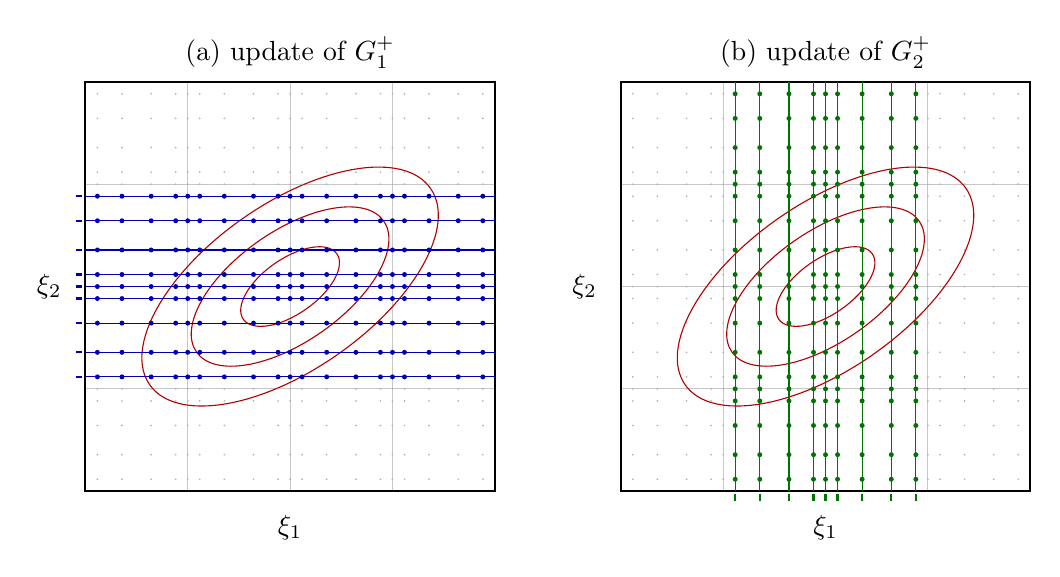
\begin{tikzpicture}
\begin{scope}[shift={(0.00,0)}]
\draw[gray!45,thin] (-2.6000,-2.6000) -- (-2.6000,2.6000);
\draw[gray!45,thin] (-2.6000,-2.6000) -- (2.6000,-2.6000);
\draw[gray!45,thin] (-1.3000,-2.6000) -- (-1.3000,2.6000);
\draw[gray!45,thin] (-2.6000,-1.3000) -- (2.6000,-1.3000);
\draw[gray!45,thin] (0.0000,-2.6000) -- (0.0000,2.6000);
\draw[gray!45,thin] (-2.6000,0.0000) -- (2.6000,0.0000);
\draw[gray!45,thin] (1.3000,-2.6000) -- (1.3000,2.6000);
\draw[gray!45,thin] (-2.6000,1.3000) -- (2.6000,1.3000);
\draw[gray!45,thin] (2.6000,-2.6000) -- (2.6000,2.6000);
\draw[gray!45,thin] (-2.6000,2.6000) -- (2.6000,2.6000);
\draw[black,thick] (-2.6000,-2.6000) rectangle (2.6000,2.6000);
\draw[red!70!black,thin,rotate=35] (0,0) ellipse (0.725 and 0.351);
\draw[red!70!black,thin,rotate=35] (0,0) ellipse (1.451 and 0.702);
\draw[red!70!black,thin,rotate=35] (0,0) ellipse (2.176 and 1.053);
\fill[gray!60] (-2.4473,-2.4473) circle (0.35pt);
\fill[gray!60] (-2.4473,-2.1354) circle (0.35pt);
\fill[gray!60] (-2.4473,-1.7646) circle (0.35pt);
\fill[gray!60] (-2.4473,-1.4527) circle (0.35pt);
\fill[gray!60] (-2.4473,-1.3000) circle (0.35pt);
\fill[gray!60] (-2.4473,-1.1473) circle (0.35pt);
\fill[gray!60] (-2.4473,-0.8354) circle (0.35pt);
\fill[gray!60] (-2.4473,-0.4646) circle (0.35pt);
\fill[gray!60] (-2.4473,-0.1527) circle (0.35pt);
\fill[gray!60] (-2.4473,0.0000) circle (0.35pt);
\fill[gray!60] (-2.4473,0.1527) circle (0.35pt);
\fill[gray!60] (-2.4473,0.4646) circle (0.35pt);
\fill[gray!60] (-2.4473,0.8354) circle (0.35pt);
\fill[gray!60] (-2.4473,1.1473) circle (0.35pt);
\fill[gray!60] (-2.4473,1.3000) circle (0.35pt);
\fill[gray!60] (-2.4473,1.4527) circle (0.35pt);
\fill[gray!60] (-2.4473,1.7646) circle (0.35pt);
\fill[gray!60] (-2.4473,2.1354) circle (0.35pt);
\fill[gray!60] (-2.4473,2.4473) circle (0.35pt);
\fill[gray!60] (-2.1354,-2.4473) circle (0.35pt);
\fill[gray!60] (-2.1354,-2.1354) circle (0.35pt);
\fill[gray!60] (-2.1354,-1.7646) circle (0.35pt);
\fill[gray!60] (-2.1354,-1.4527) circle (0.35pt);
\fill[gray!60] (-2.1354,-1.3000) circle (0.35pt);
\fill[gray!60] (-2.1354,-1.1473) circle (0.35pt);
\fill[gray!60] (-2.1354,-0.8354) circle (0.35pt);
\fill[gray!60] (-2.1354,-0.4646) circle (0.35pt);
\fill[gray!60] (-2.1354,-0.1527) circle (0.35pt);
\fill[gray!60] (-2.1354,0.0000) circle (0.35pt);
\fill[gray!60] (-2.1354,0.1527) circle (0.35pt);
\fill[gray!60] (-2.1354,0.4646) circle (0.35pt);
\fill[gray!60] (-2.1354,0.8354) circle (0.35pt);
\fill[gray!60] (-2.1354,1.1473) circle (0.35pt);
\fill[gray!60] (-2.1354,1.3000) circle (0.35pt);
\fill[gray!60] (-2.1354,1.4527) circle (0.35pt);
\fill[gray!60] (-2.1354,1.7646) circle (0.35pt);
\fill[gray!60] (-2.1354,2.1354) circle (0.35pt);
\fill[gray!60] (-2.1354,2.4473) circle (0.35pt);
\fill[gray!60] (-1.7646,-2.4473) circle (0.35pt);
\fill[gray!60] (-1.7646,-2.1354) circle (0.35pt);
\fill[gray!60] (-1.7646,-1.7646) circle (0.35pt);
\fill[gray!60] (-1.7646,-1.4527) circle (0.35pt);
\fill[gray!60] (-1.7646,-1.3000) circle (0.35pt);
\fill[gray!60] (-1.7646,-1.1473) circle (0.35pt);
\fill[gray!60] (-1.7646,-0.8354) circle (0.35pt);
\fill[gray!60] (-1.7646,-0.4646) circle (0.35pt);
\fill[gray!60] (-1.7646,-0.1527) circle (0.35pt);
\fill[gray!60] (-1.7646,0.0000) circle (0.35pt);
\fill[gray!60] (-1.7646,0.1527) circle (0.35pt);
\fill[gray!60] (-1.7646,0.4646) circle (0.35pt);
\fill[gray!60] (-1.7646,0.8354) circle (0.35pt);
\fill[gray!60] (-1.7646,1.1473) circle (0.35pt);
\fill[gray!60] (-1.7646,1.3000) circle (0.35pt);
\fill[gray!60] (-1.7646,1.4527) circle (0.35pt);
\fill[gray!60] (-1.7646,1.7646) circle (0.35pt);
\fill[gray!60] (-1.7646,2.1354) circle (0.35pt);
\fill[gray!60] (-1.7646,2.4473) circle (0.35pt);
\fill[gray!60] (-1.4527,-2.4473) circle (0.35pt);
\fill[gray!60] (-1.4527,-2.1354) circle (0.35pt);
\fill[gray!60] (-1.4527,-1.7646) circle (0.35pt);
\fill[gray!60] (-1.4527,-1.4527) circle (0.35pt);
\fill[gray!60] (-1.4527,-1.3000) circle (0.35pt);
\fill[gray!60] (-1.4527,-1.1473) circle (0.35pt);
\fill[gray!60] (-1.4527,-0.8354) circle (0.35pt);
\fill[gray!60] (-1.4527,-0.4646) circle (0.35pt);
\fill[gray!60] (-1.4527,-0.1527) circle (0.35pt);
\fill[gray!60] (-1.4527,0.0000) circle (0.35pt);
\fill[gray!60] (-1.4527,0.1527) circle (0.35pt);
\fill[gray!60] (-1.4527,0.4646) circle (0.35pt);
\fill[gray!60] (-1.4527,0.8354) circle (0.35pt);
\fill[gray!60] (-1.4527,1.1473) circle (0.35pt);
\fill[gray!60] (-1.4527,1.3000) circle (0.35pt);
\fill[gray!60] (-1.4527,1.4527) circle (0.35pt);
\fill[gray!60] (-1.4527,1.7646) circle (0.35pt);
\fill[gray!60] (-1.4527,2.1354) circle (0.35pt);
\fill[gray!60] (-1.4527,2.4473) circle (0.35pt);
\fill[gray!60] (-1.3000,-2.4473) circle (0.35pt);
\fill[gray!60] (-1.3000,-2.1354) circle (0.35pt);
\fill[gray!60] (-1.3000,-1.7646) circle (0.35pt);
\fill[gray!60] (-1.3000,-1.4527) circle (0.35pt);
\fill[gray!60] (-1.3000,-1.3000) circle (0.35pt);
\fill[gray!60] (-1.3000,-1.1473) circle (0.35pt);
\fill[gray!60] (-1.3000,-0.8354) circle (0.35pt);
\fill[gray!60] (-1.3000,-0.4646) circle (0.35pt);
\fill[gray!60] (-1.3000,-0.1527) circle (0.35pt);
\fill[gray!60] (-1.3000,0.0000) circle (0.35pt);
\fill[gray!60] (-1.3000,0.1527) circle (0.35pt);
\fill[gray!60] (-1.3000,0.4646) circle (0.35pt);
\fill[gray!60] (-1.3000,0.8354) circle (0.35pt);
\fill[gray!60] (-1.3000,1.1473) circle (0.35pt);
\fill[gray!60] (-1.3000,1.3000) circle (0.35pt);
\fill[gray!60] (-1.3000,1.4527) circle (0.35pt);
\fill[gray!60] (-1.3000,1.7646) circle (0.35pt);
\fill[gray!60] (-1.3000,2.1354) circle (0.35pt);
\fill[gray!60] (-1.3000,2.4473) circle (0.35pt);
\fill[gray!60] (-1.1473,-2.4473) circle (0.35pt);
\fill[gray!60] (-1.1473,-2.1354) circle (0.35pt);
\fill[gray!60] (-1.1473,-1.7646) circle (0.35pt);
\fill[gray!60] (-1.1473,-1.4527) circle (0.35pt);
\fill[gray!60] (-1.1473,-1.3000) circle (0.35pt);
\fill[gray!60] (-1.1473,-1.1473) circle (0.35pt);
\fill[gray!60] (-1.1473,-0.8354) circle (0.35pt);
\fill[gray!60] (-1.1473,-0.4646) circle (0.35pt);
\fill[gray!60] (-1.1473,-0.1527) circle (0.35pt);
\fill[gray!60] (-1.1473,0.0000) circle (0.35pt);
\fill[gray!60] (-1.1473,0.1527) circle (0.35pt);
\fill[gray!60] (-1.1473,0.4646) circle (0.35pt);
\fill[gray!60] (-1.1473,0.8354) circle (0.35pt);
\fill[gray!60] (-1.1473,1.1473) circle (0.35pt);
\fill[gray!60] (-1.1473,1.3000) circle (0.35pt);
\fill[gray!60] (-1.1473,1.4527) circle (0.35pt);
\fill[gray!60] (-1.1473,1.7646) circle (0.35pt);
\fill[gray!60] (-1.1473,2.1354) circle (0.35pt);
\fill[gray!60] (-1.1473,2.4473) circle (0.35pt);
\fill[gray!60] (-0.8354,-2.4473) circle (0.35pt);
\fill[gray!60] (-0.8354,-2.1354) circle (0.35pt);
\fill[gray!60] (-0.8354,-1.7646) circle (0.35pt);
\fill[gray!60] (-0.8354,-1.4527) circle (0.35pt);
\fill[gray!60] (-0.8354,-1.3000) circle (0.35pt);
\fill[gray!60] (-0.8354,-1.1473) circle (0.35pt);
\fill[gray!60] (-0.8354,-0.8354) circle (0.35pt);
\fill[gray!60] (-0.8354,-0.4646) circle (0.35pt);
\fill[gray!60] (-0.8354,-0.1527) circle (0.35pt);
\fill[gray!60] (-0.8354,0.0000) circle (0.35pt);
\fill[gray!60] (-0.8354,0.1527) circle (0.35pt);
\fill[gray!60] (-0.8354,0.4646) circle (0.35pt);
\fill[gray!60] (-0.8354,0.8354) circle (0.35pt);
\fill[gray!60] (-0.8354,1.1473) circle (0.35pt);
\fill[gray!60] (-0.8354,1.3000) circle (0.35pt);
\fill[gray!60] (-0.8354,1.4527) circle (0.35pt);
\fill[gray!60] (-0.8354,1.7646) circle (0.35pt);
\fill[gray!60] (-0.8354,2.1354) circle (0.35pt);
\fill[gray!60] (-0.8354,2.4473) circle (0.35pt);
\fill[gray!60] (-0.4646,-2.4473) circle (0.35pt);
\fill[gray!60] (-0.4646,-2.1354) circle (0.35pt);
\fill[gray!60] (-0.4646,-1.7646) circle (0.35pt);
\fill[gray!60] (-0.4646,-1.4527) circle (0.35pt);
\fill[gray!60] (-0.4646,-1.3000) circle (0.35pt);
\fill[gray!60] (-0.4646,-1.1473) circle (0.35pt);
\fill[gray!60] (-0.4646,-0.8354) circle (0.35pt);
\fill[gray!60] (-0.4646,-0.4646) circle (0.35pt);
\fill[gray!60] (-0.4646,-0.1527) circle (0.35pt);
\fill[gray!60] (-0.4646,0.0000) circle (0.35pt);
\fill[gray!60] (-0.4646,0.1527) circle (0.35pt);
\fill[gray!60] (-0.4646,0.4646) circle (0.35pt);
\fill[gray!60] (-0.4646,0.8354) circle (0.35pt);
\fill[gray!60] (-0.4646,1.1473) circle (0.35pt);
\fill[gray!60] (-0.4646,1.3000) circle (0.35pt);
\fill[gray!60] (-0.4646,1.4527) circle (0.35pt);
\fill[gray!60] (-0.4646,1.7646) circle (0.35pt);
\fill[gray!60] (-0.4646,2.1354) circle (0.35pt);
\fill[gray!60] (-0.4646,2.4473) circle (0.35pt);
\fill[gray!60] (-0.1527,-2.4473) circle (0.35pt);
\fill[gray!60] (-0.1527,-2.1354) circle (0.35pt);
\fill[gray!60] (-0.1527,-1.7646) circle (0.35pt);
\fill[gray!60] (-0.1527,-1.4527) circle (0.35pt);
\fill[gray!60] (-0.1527,-1.3000) circle (0.35pt);
\fill[gray!60] (-0.1527,-1.1473) circle (0.35pt);
\fill[gray!60] (-0.1527,-0.8354) circle (0.35pt);
\fill[gray!60] (-0.1527,-0.4646) circle (0.35pt);
\fill[gray!60] (-0.1527,-0.1527) circle (0.35pt);
\fill[gray!60] (-0.1527,0.0000) circle (0.35pt);
\fill[gray!60] (-0.1527,0.1527) circle (0.35pt);
\fill[gray!60] (-0.1527,0.4646) circle (0.35pt);
\fill[gray!60] (-0.1527,0.8354) circle (0.35pt);
\fill[gray!60] (-0.1527,1.1473) circle (0.35pt);
\fill[gray!60] (-0.1527,1.3000) circle (0.35pt);
\fill[gray!60] (-0.1527,1.4527) circle (0.35pt);
\fill[gray!60] (-0.1527,1.7646) circle (0.35pt);
\fill[gray!60] (-0.1527,2.1354) circle (0.35pt);
\fill[gray!60] (-0.1527,2.4473) circle (0.35pt);
\fill[gray!60] (0.0000,-2.4473) circle (0.35pt);
\fill[gray!60] (0.0000,-2.1354) circle (0.35pt);
\fill[gray!60] (0.0000,-1.7646) circle (0.35pt);
\fill[gray!60] (0.0000,-1.4527) circle (0.35pt);
\fill[gray!60] (0.0000,-1.3000) circle (0.35pt);
\fill[gray!60] (0.0000,-1.1473) circle (0.35pt);
\fill[gray!60] (0.0000,-0.8354) circle (0.35pt);
\fill[gray!60] (0.0000,-0.4646) circle (0.35pt);
\fill[gray!60] (0.0000,-0.1527) circle (0.35pt);
\fill[gray!60] (0.0000,0.0000) circle (0.35pt);
\fill[gray!60] (0.0000,0.1527) circle (0.35pt);
\fill[gray!60] (0.0000,0.4646) circle (0.35pt);
\fill[gray!60] (0.0000,0.8354) circle (0.35pt);
\fill[gray!60] (0.0000,1.1473) circle (0.35pt);
\fill[gray!60] (0.0000,1.3000) circle (0.35pt);
\fill[gray!60] (0.0000,1.4527) circle (0.35pt);
\fill[gray!60] (0.0000,1.7646) circle (0.35pt);
\fill[gray!60] (0.0000,2.1354) circle (0.35pt);
\fill[gray!60] (0.0000,2.4473) circle (0.35pt);
\fill[gray!60] (0.1527,-2.4473) circle (0.35pt);
\fill[gray!60] (0.1527,-2.1354) circle (0.35pt);
\fill[gray!60] (0.1527,-1.7646) circle (0.35pt);
\fill[gray!60] (0.1527,-1.4527) circle (0.35pt);
\fill[gray!60] (0.1527,-1.3000) circle (0.35pt);
\fill[gray!60] (0.1527,-1.1473) circle (0.35pt);
\fill[gray!60] (0.1527,-0.8354) circle (0.35pt);
\fill[gray!60] (0.1527,-0.4646) circle (0.35pt);
\fill[gray!60] (0.1527,-0.1527) circle (0.35pt);
\fill[gray!60] (0.1527,0.0000) circle (0.35pt);
\fill[gray!60] (0.1527,0.1527) circle (0.35pt);
\fill[gray!60] (0.1527,0.4646) circle (0.35pt);
\fill[gray!60] (0.1527,0.8354) circle (0.35pt);
\fill[gray!60] (0.1527,1.1473) circle (0.35pt);
\fill[gray!60] (0.1527,1.3000) circle (0.35pt);
\fill[gray!60] (0.1527,1.4527) circle (0.35pt);
\fill[gray!60] (0.1527,1.7646) circle (0.35pt);
\fill[gray!60] (0.1527,2.1354) circle (0.35pt);
\fill[gray!60] (0.1527,2.4473) circle (0.35pt);
\fill[gray!60] (0.4646,-2.4473) circle (0.35pt);
\fill[gray!60] (0.4646,-2.1354) circle (0.35pt);
\fill[gray!60] (0.4646,-1.7646) circle (0.35pt);
\fill[gray!60] (0.4646,-1.4527) circle (0.35pt);
\fill[gray!60] (0.4646,-1.3000) circle (0.35pt);
\fill[gray!60] (0.4646,-1.1473) circle (0.35pt);
\fill[gray!60] (0.4646,-0.8354) circle (0.35pt);
\fill[gray!60] (0.4646,-0.4646) circle (0.35pt);
\fill[gray!60] (0.4646,-0.1527) circle (0.35pt);
\fill[gray!60] (0.4646,0.0000) circle (0.35pt);
\fill[gray!60] (0.4646,0.1527) circle (0.35pt);
\fill[gray!60] (0.4646,0.4646) circle (0.35pt);
\fill[gray!60] (0.4646,0.8354) circle (0.35pt);
\fill[gray!60] (0.4646,1.1473) circle (0.35pt);
\fill[gray!60] (0.4646,1.3000) circle (0.35pt);
\fill[gray!60] (0.4646,1.4527) circle (0.35pt);
\fill[gray!60] (0.4646,1.7646) circle (0.35pt);
\fill[gray!60] (0.4646,2.1354) circle (0.35pt);
\fill[gray!60] (0.4646,2.4473) circle (0.35pt);
\fill[gray!60] (0.8354,-2.4473) circle (0.35pt);
\fill[gray!60] (0.8354,-2.1354) circle (0.35pt);
\fill[gray!60] (0.8354,-1.7646) circle (0.35pt);
\fill[gray!60] (0.8354,-1.4527) circle (0.35pt);
\fill[gray!60] (0.8354,-1.3000) circle (0.35pt);
\fill[gray!60] (0.8354,-1.1473) circle (0.35pt);
\fill[gray!60] (0.8354,-0.8354) circle (0.35pt);
\fill[gray!60] (0.8354,-0.4646) circle (0.35pt);
\fill[gray!60] (0.8354,-0.1527) circle (0.35pt);
\fill[gray!60] (0.8354,0.0000) circle (0.35pt);
\fill[gray!60] (0.8354,0.1527) circle (0.35pt);
\fill[gray!60] (0.8354,0.4646) circle (0.35pt);
\fill[gray!60] (0.8354,0.8354) circle (0.35pt);
\fill[gray!60] (0.8354,1.1473) circle (0.35pt);
\fill[gray!60] (0.8354,1.3000) circle (0.35pt);
\fill[gray!60] (0.8354,1.4527) circle (0.35pt);
\fill[gray!60] (0.8354,1.7646) circle (0.35pt);
\fill[gray!60] (0.8354,2.1354) circle (0.35pt);
\fill[gray!60] (0.8354,2.4473) circle (0.35pt);
\fill[gray!60] (1.1473,-2.4473) circle (0.35pt);
\fill[gray!60] (1.1473,-2.1354) circle (0.35pt);
\fill[gray!60] (1.1473,-1.7646) circle (0.35pt);
\fill[gray!60] (1.1473,-1.4527) circle (0.35pt);
\fill[gray!60] (1.1473,-1.3000) circle (0.35pt);
\fill[gray!60] (1.1473,-1.1473) circle (0.35pt);
\fill[gray!60] (1.1473,-0.8354) circle (0.35pt);
\fill[gray!60] (1.1473,-0.4646) circle (0.35pt);
\fill[gray!60] (1.1473,-0.1527) circle (0.35pt);
\fill[gray!60] (1.1473,0.0000) circle (0.35pt);
\fill[gray!60] (1.1473,0.1527) circle (0.35pt);
\fill[gray!60] (1.1473,0.4646) circle (0.35pt);
\fill[gray!60] (1.1473,0.8354) circle (0.35pt);
\fill[gray!60] (1.1473,1.1473) circle (0.35pt);
\fill[gray!60] (1.1473,1.3000) circle (0.35pt);
\fill[gray!60] (1.1473,1.4527) circle (0.35pt);
\fill[gray!60] (1.1473,1.7646) circle (0.35pt);
\fill[gray!60] (1.1473,2.1354) circle (0.35pt);
\fill[gray!60] (1.1473,2.4473) circle (0.35pt);
\fill[gray!60] (1.3000,-2.4473) circle (0.35pt);
\fill[gray!60] (1.3000,-2.1354) circle (0.35pt);
\fill[gray!60] (1.3000,-1.7646) circle (0.35pt);
\fill[gray!60] (1.3000,-1.4527) circle (0.35pt);
\fill[gray!60] (1.3000,-1.3000) circle (0.35pt);
\fill[gray!60] (1.3000,-1.1473) circle (0.35pt);
\fill[gray!60] (1.3000,-0.8354) circle (0.35pt);
\fill[gray!60] (1.3000,-0.4646) circle (0.35pt);
\fill[gray!60] (1.3000,-0.1527) circle (0.35pt);
\fill[gray!60] (1.3000,0.0000) circle (0.35pt);
\fill[gray!60] (1.3000,0.1527) circle (0.35pt);
\fill[gray!60] (1.3000,0.4646) circle (0.35pt);
\fill[gray!60] (1.3000,0.8354) circle (0.35pt);
\fill[gray!60] (1.3000,1.1473) circle (0.35pt);
\fill[gray!60] (1.3000,1.3000) circle (0.35pt);
\fill[gray!60] (1.3000,1.4527) circle (0.35pt);
\fill[gray!60] (1.3000,1.7646) circle (0.35pt);
\fill[gray!60] (1.3000,2.1354) circle (0.35pt);
\fill[gray!60] (1.3000,2.4473) circle (0.35pt);
\fill[gray!60] (1.4527,-2.4473) circle (0.35pt);
\fill[gray!60] (1.4527,-2.1354) circle (0.35pt);
\fill[gray!60] (1.4527,-1.7646) circle (0.35pt);
\fill[gray!60] (1.4527,-1.4527) circle (0.35pt);
\fill[gray!60] (1.4527,-1.3000) circle (0.35pt);
\fill[gray!60] (1.4527,-1.1473) circle (0.35pt);
\fill[gray!60] (1.4527,-0.8354) circle (0.35pt);
\fill[gray!60] (1.4527,-0.4646) circle (0.35pt);
\fill[gray!60] (1.4527,-0.1527) circle (0.35pt);
\fill[gray!60] (1.4527,0.0000) circle (0.35pt);
\fill[gray!60] (1.4527,0.1527) circle (0.35pt);
\fill[gray!60] (1.4527,0.4646) circle (0.35pt);
\fill[gray!60] (1.4527,0.8354) circle (0.35pt);
\fill[gray!60] (1.4527,1.1473) circle (0.35pt);
\fill[gray!60] (1.4527,1.3000) circle (0.35pt);
\fill[gray!60] (1.4527,1.4527) circle (0.35pt);
\fill[gray!60] (1.4527,1.7646) circle (0.35pt);
\fill[gray!60] (1.4527,2.1354) circle (0.35pt);
\fill[gray!60] (1.4527,2.4473) circle (0.35pt);
\fill[gray!60] (1.7646,-2.4473) circle (0.35pt);
\fill[gray!60] (1.7646,-2.1354) circle (0.35pt);
\fill[gray!60] (1.7646,-1.7646) circle (0.35pt);
\fill[gray!60] (1.7646,-1.4527) circle (0.35pt);
\fill[gray!60] (1.7646,-1.3000) circle (0.35pt);
\fill[gray!60] (1.7646,-1.1473) circle (0.35pt);
\fill[gray!60] (1.7646,-0.8354) circle (0.35pt);
\fill[gray!60] (1.7646,-0.4646) circle (0.35pt);
\fill[gray!60] (1.7646,-0.1527) circle (0.35pt);
\fill[gray!60] (1.7646,0.0000) circle (0.35pt);
\fill[gray!60] (1.7646,0.1527) circle (0.35pt);
\fill[gray!60] (1.7646,0.4646) circle (0.35pt);
\fill[gray!60] (1.7646,0.8354) circle (0.35pt);
\fill[gray!60] (1.7646,1.1473) circle (0.35pt);
\fill[gray!60] (1.7646,1.3000) circle (0.35pt);
\fill[gray!60] (1.7646,1.4527) circle (0.35pt);
\fill[gray!60] (1.7646,1.7646) circle (0.35pt);
\fill[gray!60] (1.7646,2.1354) circle (0.35pt);
\fill[gray!60] (1.7646,2.4473) circle (0.35pt);
\fill[gray!60] (2.1354,-2.4473) circle (0.35pt);
\fill[gray!60] (2.1354,-2.1354) circle (0.35pt);
\fill[gray!60] (2.1354,-1.7646) circle (0.35pt);
\fill[gray!60] (2.1354,-1.4527) circle (0.35pt);
\fill[gray!60] (2.1354,-1.3000) circle (0.35pt);
\fill[gray!60] (2.1354,-1.1473) circle (0.35pt);
\fill[gray!60] (2.1354,-0.8354) circle (0.35pt);
\fill[gray!60] (2.1354,-0.4646) circle (0.35pt);
\fill[gray!60] (2.1354,-0.1527) circle (0.35pt);
\fill[gray!60] (2.1354,0.0000) circle (0.35pt);
\fill[gray!60] (2.1354,0.1527) circle (0.35pt);
\fill[gray!60] (2.1354,0.4646) circle (0.35pt);
\fill[gray!60] (2.1354,0.8354) circle (0.35pt);
\fill[gray!60] (2.1354,1.1473) circle (0.35pt);
\fill[gray!60] (2.1354,1.3000) circle (0.35pt);
\fill[gray!60] (2.1354,1.4527) circle (0.35pt);
\fill[gray!60] (2.1354,1.7646) circle (0.35pt);
\fill[gray!60] (2.1354,2.1354) circle (0.35pt);
\fill[gray!60] (2.1354,2.4473) circle (0.35pt);
\fill[gray!60] (2.4473,-2.4473) circle (0.35pt);
\fill[gray!60] (2.4473,-2.1354) circle (0.35pt);
\fill[gray!60] (2.4473,-1.7646) circle (0.35pt);
\fill[gray!60] (2.4473,-1.4527) circle (0.35pt);
\fill[gray!60] (2.4473,-1.3000) circle (0.35pt);
\fill[gray!60] (2.4473,-1.1473) circle (0.35pt);
\fill[gray!60] (2.4473,-0.8354) circle (0.35pt);
\fill[gray!60] (2.4473,-0.4646) circle (0.35pt);
\fill[gray!60] (2.4473,-0.1527) circle (0.35pt);
\fill[gray!60] (2.4473,0.0000) circle (0.35pt);
\fill[gray!60] (2.4473,0.1527) circle (0.35pt);
\fill[gray!60] (2.4473,0.4646) circle (0.35pt);
\fill[gray!60] (2.4473,0.8354) circle (0.35pt);
\fill[gray!60] (2.4473,1.1473) circle (0.35pt);
\fill[gray!60] (2.4473,1.3000) circle (0.35pt);
\fill[gray!60] (2.4473,1.4527) circle (0.35pt);
\fill[gray!60] (2.4473,1.7646) circle (0.35pt);
\fill[gray!60] (2.4473,2.1354) circle (0.35pt);
\fill[gray!60] (2.4473,2.4473) circle (0.35pt);
\draw[blue!70!black,line width=0.4pt] (-2.6000,-1.1473) -- (2.6000,-1.1473);
\fill[blue!70!black] (-2.4473,-1.1473) circle (0.9pt);
\fill[blue!70!black] (-2.1354,-1.1473) circle (0.9pt);
\fill[blue!70!black] (-1.7646,-1.1473) circle (0.9pt);
\fill[blue!70!black] (-1.4527,-1.1473) circle (0.9pt);
\fill[blue!70!black] (-1.3000,-1.1473) circle (0.9pt);
\fill[blue!70!black] (-1.1473,-1.1473) circle (0.9pt);
\fill[blue!70!black] (-0.8354,-1.1473) circle (0.9pt);
\fill[blue!70!black] (-0.4646,-1.1473) circle (0.9pt);
\fill[blue!70!black] (-0.1527,-1.1473) circle (0.9pt);
\fill[blue!70!black] (0.0000,-1.1473) circle (0.9pt);
\fill[blue!70!black] (0.1527,-1.1473) circle (0.9pt);
\fill[blue!70!black] (0.4646,-1.1473) circle (0.9pt);
\fill[blue!70!black] (0.8354,-1.1473) circle (0.9pt);
\fill[blue!70!black] (1.1473,-1.1473) circle (0.9pt);
\fill[blue!70!black] (1.3000,-1.1473) circle (0.9pt);
\fill[blue!70!black] (1.4527,-1.1473) circle (0.9pt);
\fill[blue!70!black] (1.7646,-1.1473) circle (0.9pt);
\fill[blue!70!black] (2.1354,-1.1473) circle (0.9pt);
\fill[blue!70!black] (2.4473,-1.1473) circle (0.9pt);
\draw[blue!70!black,thick] (-2.7200,-1.1473) -- (-2.6400,-1.1473);
\draw[blue!70!black,line width=0.4pt] (-2.6000,-0.8354) -- (2.6000,-0.8354);
\fill[blue!70!black] (-2.4473,-0.8354) circle (0.9pt);
\fill[blue!70!black] (-2.1354,-0.8354) circle (0.9pt);
\fill[blue!70!black] (-1.7646,-0.8354) circle (0.9pt);
\fill[blue!70!black] (-1.4527,-0.8354) circle (0.9pt);
\fill[blue!70!black] (-1.3000,-0.8354) circle (0.9pt);
\fill[blue!70!black] (-1.1473,-0.8354) circle (0.9pt);
\fill[blue!70!black] (-0.8354,-0.8354) circle (0.9pt);
\fill[blue!70!black] (-0.4646,-0.8354) circle (0.9pt);
\fill[blue!70!black] (-0.1527,-0.8354) circle (0.9pt);
\fill[blue!70!black] (0.0000,-0.8354) circle (0.9pt);
\fill[blue!70!black] (0.1527,-0.8354) circle (0.9pt);
\fill[blue!70!black] (0.4646,-0.8354) circle (0.9pt);
\fill[blue!70!black] (0.8354,-0.8354) circle (0.9pt);
\fill[blue!70!black] (1.1473,-0.8354) circle (0.9pt);
\fill[blue!70!black] (1.3000,-0.8354) circle (0.9pt);
\fill[blue!70!black] (1.4527,-0.8354) circle (0.9pt);
\fill[blue!70!black] (1.7646,-0.8354) circle (0.9pt);
\fill[blue!70!black] (2.1354,-0.8354) circle (0.9pt);
\fill[blue!70!black] (2.4473,-0.8354) circle (0.9pt);
\draw[blue!70!black,thick] (-2.7200,-0.8354) -- (-2.6400,-0.8354);
\draw[blue!70!black,line width=0.4pt] (-2.6000,-0.4646) -- (2.6000,-0.4646);
\fill[blue!70!black] (-2.4473,-0.4646) circle (0.9pt);
\fill[blue!70!black] (-2.1354,-0.4646) circle (0.9pt);
\fill[blue!70!black] (-1.7646,-0.4646) circle (0.9pt);
\fill[blue!70!black] (-1.4527,-0.4646) circle (0.9pt);
\fill[blue!70!black] (-1.3000,-0.4646) circle (0.9pt);
\fill[blue!70!black] (-1.1473,-0.4646) circle (0.9pt);
\fill[blue!70!black] (-0.8354,-0.4646) circle (0.9pt);
\fill[blue!70!black] (-0.4646,-0.4646) circle (0.9pt);
\fill[blue!70!black] (-0.1527,-0.4646) circle (0.9pt);
\fill[blue!70!black] (0.0000,-0.4646) circle (0.9pt);
\fill[blue!70!black] (0.1527,-0.4646) circle (0.9pt);
\fill[blue!70!black] (0.4646,-0.4646) circle (0.9pt);
\fill[blue!70!black] (0.8354,-0.4646) circle (0.9pt);
\fill[blue!70!black] (1.1473,-0.4646) circle (0.9pt);
\fill[blue!70!black] (1.3000,-0.4646) circle (0.9pt);
\fill[blue!70!black] (1.4527,-0.4646) circle (0.9pt);
\fill[blue!70!black] (1.7646,-0.4646) circle (0.9pt);
\fill[blue!70!black] (2.1354,-0.4646) circle (0.9pt);
\fill[blue!70!black] (2.4473,-0.4646) circle (0.9pt);
\draw[blue!70!black,thick] (-2.7200,-0.4646) -- (-2.6400,-0.4646);
\draw[blue!70!black,line width=0.4pt] (-2.6000,-0.1527) -- (2.6000,-0.1527);
\fill[blue!70!black] (-2.4473,-0.1527) circle (0.9pt);
\fill[blue!70!black] (-2.1354,-0.1527) circle (0.9pt);
\fill[blue!70!black] (-1.7646,-0.1527) circle (0.9pt);
\fill[blue!70!black] (-1.4527,-0.1527) circle (0.9pt);
\fill[blue!70!black] (-1.3000,-0.1527) circle (0.9pt);
\fill[blue!70!black] (-1.1473,-0.1527) circle (0.9pt);
\fill[blue!70!black] (-0.8354,-0.1527) circle (0.9pt);
\fill[blue!70!black] (-0.4646,-0.1527) circle (0.9pt);
\fill[blue!70!black] (-0.1527,-0.1527) circle (0.9pt);
\fill[blue!70!black] (0.0000,-0.1527) circle (0.9pt);
\fill[blue!70!black] (0.1527,-0.1527) circle (0.9pt);
\fill[blue!70!black] (0.4646,-0.1527) circle (0.9pt);
\fill[blue!70!black] (0.8354,-0.1527) circle (0.9pt);
\fill[blue!70!black] (1.1473,-0.1527) circle (0.9pt);
\fill[blue!70!black] (1.3000,-0.1527) circle (0.9pt);
\fill[blue!70!black] (1.4527,-0.1527) circle (0.9pt);
\fill[blue!70!black] (1.7646,-0.1527) circle (0.9pt);
\fill[blue!70!black] (2.1354,-0.1527) circle (0.9pt);
\fill[blue!70!black] (2.4473,-0.1527) circle (0.9pt);
\draw[blue!70!black,thick] (-2.7200,-0.1527) -- (-2.6400,-0.1527);
\draw[blue!70!black,line width=0.4pt] (-2.6000,0.0000) -- (2.6000,0.0000);
\fill[blue!70!black] (-2.4473,0.0000) circle (0.9pt);
\fill[blue!70!black] (-2.1354,0.0000) circle (0.9pt);
\fill[blue!70!black] (-1.7646,0.0000) circle (0.9pt);
\fill[blue!70!black] (-1.4527,0.0000) circle (0.9pt);
\fill[blue!70!black] (-1.3000,0.0000) circle (0.9pt);
\fill[blue!70!black] (-1.1473,0.0000) circle (0.9pt);
\fill[blue!70!black] (-0.8354,0.0000) circle (0.9pt);
\fill[blue!70!black] (-0.4646,0.0000) circle (0.9pt);
\fill[blue!70!black] (-0.1527,0.0000) circle (0.9pt);
\fill[blue!70!black] (0.0000,0.0000) circle (0.9pt);
\fill[blue!70!black] (0.1527,0.0000) circle (0.9pt);
\fill[blue!70!black] (0.4646,0.0000) circle (0.9pt);
\fill[blue!70!black] (0.8354,0.0000) circle (0.9pt);
\fill[blue!70!black] (1.1473,0.0000) circle (0.9pt);
\fill[blue!70!black] (1.3000,0.0000) circle (0.9pt);
\fill[blue!70!black] (1.4527,0.0000) circle (0.9pt);
\fill[blue!70!black] (1.7646,0.0000) circle (0.9pt);
\fill[blue!70!black] (2.1354,0.0000) circle (0.9pt);
\fill[blue!70!black] (2.4473,0.0000) circle (0.9pt);
\draw[blue!70!black,thick] (-2.7200,0.0000) -- (-2.6400,0.0000);
\draw[blue!70!black,line width=0.4pt] (-2.6000,0.1527) -- (2.6000,0.1527);
\fill[blue!70!black] (-2.4473,0.1527) circle (0.9pt);
\fill[blue!70!black] (-2.1354,0.1527) circle (0.9pt);
\fill[blue!70!black] (-1.7646,0.1527) circle (0.9pt);
\fill[blue!70!black] (-1.4527,0.1527) circle (0.9pt);
\fill[blue!70!black] (-1.3000,0.1527) circle (0.9pt);
\fill[blue!70!black] (-1.1473,0.1527) circle (0.9pt);
\fill[blue!70!black] (-0.8354,0.1527) circle (0.9pt);
\fill[blue!70!black] (-0.4646,0.1527) circle (0.9pt);
\fill[blue!70!black] (-0.1527,0.1527) circle (0.9pt);
\fill[blue!70!black] (0.0000,0.1527) circle (0.9pt);
\fill[blue!70!black] (0.1527,0.1527) circle (0.9pt);
\fill[blue!70!black] (0.4646,0.1527) circle (0.9pt);
\fill[blue!70!black] (0.8354,0.1527) circle (0.9pt);
\fill[blue!70!black] (1.1473,0.1527) circle (0.9pt);
\fill[blue!70!black] (1.3000,0.1527) circle (0.9pt);
\fill[blue!70!black] (1.4527,0.1527) circle (0.9pt);
\fill[blue!70!black] (1.7646,0.1527) circle (0.9pt);
\fill[blue!70!black] (2.1354,0.1527) circle (0.9pt);
\fill[blue!70!black] (2.4473,0.1527) circle (0.9pt);
\draw[blue!70!black,thick] (-2.7200,0.1527) -- (-2.6400,0.1527);
\draw[blue!70!black,line width=0.4pt] (-2.6000,0.4646) -- (2.6000,0.4646);
\fill[blue!70!black] (-2.4473,0.4646) circle (0.9pt);
\fill[blue!70!black] (-2.1354,0.4646) circle (0.9pt);
\fill[blue!70!black] (-1.7646,0.4646) circle (0.9pt);
\fill[blue!70!black] (-1.4527,0.4646) circle (0.9pt);
\fill[blue!70!black] (-1.3000,0.4646) circle (0.9pt);
\fill[blue!70!black] (-1.1473,0.4646) circle (0.9pt);
\fill[blue!70!black] (-0.8354,0.4646) circle (0.9pt);
\fill[blue!70!black] (-0.4646,0.4646) circle (0.9pt);
\fill[blue!70!black] (-0.1527,0.4646) circle (0.9pt);
\fill[blue!70!black] (0.0000,0.4646) circle (0.9pt);
\fill[blue!70!black] (0.1527,0.4646) circle (0.9pt);
\fill[blue!70!black] (0.4646,0.4646) circle (0.9pt);
\fill[blue!70!black] (0.8354,0.4646) circle (0.9pt);
\fill[blue!70!black] (1.1473,0.4646) circle (0.9pt);
\fill[blue!70!black] (1.3000,0.4646) circle (0.9pt);
\fill[blue!70!black] (1.4527,0.4646) circle (0.9pt);
\fill[blue!70!black] (1.7646,0.4646) circle (0.9pt);
\fill[blue!70!black] (2.1354,0.4646) circle (0.9pt);
\fill[blue!70!black] (2.4473,0.4646) circle (0.9pt);
\draw[blue!70!black,thick] (-2.7200,0.4646) -- (-2.6400,0.4646);
\draw[blue!70!black,line width=0.4pt] (-2.6000,0.8354) -- (2.6000,0.8354);
\fill[blue!70!black] (-2.4473,0.8354) circle (0.9pt);
\fill[blue!70!black] (-2.1354,0.8354) circle (0.9pt);
\fill[blue!70!black] (-1.7646,0.8354) circle (0.9pt);
\fill[blue!70!black] (-1.4527,0.8354) circle (0.9pt);
\fill[blue!70!black] (-1.3000,0.8354) circle (0.9pt);
\fill[blue!70!black] (-1.1473,0.8354) circle (0.9pt);
\fill[blue!70!black] (-0.8354,0.8354) circle (0.9pt);
\fill[blue!70!black] (-0.4646,0.8354) circle (0.9pt);
\fill[blue!70!black] (-0.1527,0.8354) circle (0.9pt);
\fill[blue!70!black] (0.0000,0.8354) circle (0.9pt);
\fill[blue!70!black] (0.1527,0.8354) circle (0.9pt);
\fill[blue!70!black] (0.4646,0.8354) circle (0.9pt);
\fill[blue!70!black] (0.8354,0.8354) circle (0.9pt);
\fill[blue!70!black] (1.1473,0.8354) circle (0.9pt);
\fill[blue!70!black] (1.3000,0.8354) circle (0.9pt);
\fill[blue!70!black] (1.4527,0.8354) circle (0.9pt);
\fill[blue!70!black] (1.7646,0.8354) circle (0.9pt);
\fill[blue!70!black] (2.1354,0.8354) circle (0.9pt);
\fill[blue!70!black] (2.4473,0.8354) circle (0.9pt);
\draw[blue!70!black,thick] (-2.7200,0.8354) -- (-2.6400,0.8354);
\draw[blue!70!black,line width=0.4pt] (-2.6000,1.1473) -- (2.6000,1.1473);
\fill[blue!70!black] (-2.4473,1.1473) circle (0.9pt);
\fill[blue!70!black] (-2.1354,1.1473) circle (0.9pt);
\fill[blue!70!black] (-1.7646,1.1473) circle (0.9pt);
\fill[blue!70!black] (-1.4527,1.1473) circle (0.9pt);
\fill[blue!70!black] (-1.3000,1.1473) circle (0.9pt);
\fill[blue!70!black] (-1.1473,1.1473) circle (0.9pt);
\fill[blue!70!black] (-0.8354,1.1473) circle (0.9pt);
\fill[blue!70!black] (-0.4646,1.1473) circle (0.9pt);
\fill[blue!70!black] (-0.1527,1.1473) circle (0.9pt);
\fill[blue!70!black] (0.0000,1.1473) circle (0.9pt);
\fill[blue!70!black] (0.1527,1.1473) circle (0.9pt);
\fill[blue!70!black] (0.4646,1.1473) circle (0.9pt);
\fill[blue!70!black] (0.8354,1.1473) circle (0.9pt);
\fill[blue!70!black] (1.1473,1.1473) circle (0.9pt);
\fill[blue!70!black] (1.3000,1.1473) circle (0.9pt);
\fill[blue!70!black] (1.4527,1.1473) circle (0.9pt);
\fill[blue!70!black] (1.7646,1.1473) circle (0.9pt);
\fill[blue!70!black] (2.1354,1.1473) circle (0.9pt);
\fill[blue!70!black] (2.4473,1.1473) circle (0.9pt);
\draw[blue!70!black,thick] (-2.7200,1.1473) -- (-2.6400,1.1473);
\node[below] at (0.000,-2.780) {$\xi_1$};
\node[left] at (-2.780,0.000) {$\xi_2$};
\node[above] at (0,2.650) {(a) update of $G_1^+$};
\end{scope}
\begin{scope}[shift={(6.80,0)}]
\draw[gray!45,thin] (-2.6000,-2.6000) -- (-2.6000,2.6000);
\draw[gray!45,thin] (-2.6000,-2.6000) -- (2.6000,-2.6000);
\draw[gray!45,thin] (-1.3000,-2.6000) -- (-1.3000,2.6000);
\draw[gray!45,thin] (-2.6000,-1.3000) -- (2.6000,-1.3000);
\draw[gray!45,thin] (0.0000,-2.6000) -- (0.0000,2.6000);
\draw[gray!45,thin] (-2.6000,0.0000) -- (2.6000,0.0000);
\draw[gray!45,thin] (1.3000,-2.6000) -- (1.3000,2.6000);
\draw[gray!45,thin] (-2.6000,1.3000) -- (2.6000,1.3000);
\draw[gray!45,thin] (2.6000,-2.6000) -- (2.6000,2.6000);
\draw[gray!45,thin] (-2.6000,2.6000) -- (2.6000,2.6000);
\draw[black,thick] (-2.6000,-2.6000) rectangle (2.6000,2.6000);
\draw[red!70!black,thin,rotate=35] (0,0) ellipse (0.725 and 0.351);
\draw[red!70!black,thin,rotate=35] (0,0) ellipse (1.451 and 0.702);
\draw[red!70!black,thin,rotate=35] (0,0) ellipse (2.176 and 1.053);
\fill[gray!60] (-2.4473,-2.4473) circle (0.35pt);
\fill[gray!60] (-2.4473,-2.1354) circle (0.35pt);
\fill[gray!60] (-2.4473,-1.7646) circle (0.35pt);
\fill[gray!60] (-2.4473,-1.4527) circle (0.35pt);
\fill[gray!60] (-2.4473,-1.3000) circle (0.35pt);
\fill[gray!60] (-2.4473,-1.1473) circle (0.35pt);
\fill[gray!60] (-2.4473,-0.8354) circle (0.35pt);
\fill[gray!60] (-2.4473,-0.4646) circle (0.35pt);
\fill[gray!60] (-2.4473,-0.1527) circle (0.35pt);
\fill[gray!60] (-2.4473,0.0000) circle (0.35pt);
\fill[gray!60] (-2.4473,0.1527) circle (0.35pt);
\fill[gray!60] (-2.4473,0.4646) circle (0.35pt);
\fill[gray!60] (-2.4473,0.8354) circle (0.35pt);
\fill[gray!60] (-2.4473,1.1473) circle (0.35pt);
\fill[gray!60] (-2.4473,1.3000) circle (0.35pt);
\fill[gray!60] (-2.4473,1.4527) circle (0.35pt);
\fill[gray!60] (-2.4473,1.7646) circle (0.35pt);
\fill[gray!60] (-2.4473,2.1354) circle (0.35pt);
\fill[gray!60] (-2.4473,2.4473) circle (0.35pt);
\fill[gray!60] (-2.1354,-2.4473) circle (0.35pt);
\fill[gray!60] (-2.1354,-2.1354) circle (0.35pt);
\fill[gray!60] (-2.1354,-1.7646) circle (0.35pt);
\fill[gray!60] (-2.1354,-1.4527) circle (0.35pt);
\fill[gray!60] (-2.1354,-1.3000) circle (0.35pt);
\fill[gray!60] (-2.1354,-1.1473) circle (0.35pt);
\fill[gray!60] (-2.1354,-0.8354) circle (0.35pt);
\fill[gray!60] (-2.1354,-0.4646) circle (0.35pt);
\fill[gray!60] (-2.1354,-0.1527) circle (0.35pt);
\fill[gray!60] (-2.1354,0.0000) circle (0.35pt);
\fill[gray!60] (-2.1354,0.1527) circle (0.35pt);
\fill[gray!60] (-2.1354,0.4646) circle (0.35pt);
\fill[gray!60] (-2.1354,0.8354) circle (0.35pt);
\fill[gray!60] (-2.1354,1.1473) circle (0.35pt);
\fill[gray!60] (-2.1354,1.3000) circle (0.35pt);
\fill[gray!60] (-2.1354,1.4527) circle (0.35pt);
\fill[gray!60] (-2.1354,1.7646) circle (0.35pt);
\fill[gray!60] (-2.1354,2.1354) circle (0.35pt);
\fill[gray!60] (-2.1354,2.4473) circle (0.35pt);
\fill[gray!60] (-1.7646,-2.4473) circle (0.35pt);
\fill[gray!60] (-1.7646,-2.1354) circle (0.35pt);
\fill[gray!60] (-1.7646,-1.7646) circle (0.35pt);
\fill[gray!60] (-1.7646,-1.4527) circle (0.35pt);
\fill[gray!60] (-1.7646,-1.3000) circle (0.35pt);
\fill[gray!60] (-1.7646,-1.1473) circle (0.35pt);
\fill[gray!60] (-1.7646,-0.8354) circle (0.35pt);
\fill[gray!60] (-1.7646,-0.4646) circle (0.35pt);
\fill[gray!60] (-1.7646,-0.1527) circle (0.35pt);
\fill[gray!60] (-1.7646,0.0000) circle (0.35pt);
\fill[gray!60] (-1.7646,0.1527) circle (0.35pt);
\fill[gray!60] (-1.7646,0.4646) circle (0.35pt);
\fill[gray!60] (-1.7646,0.8354) circle (0.35pt);
\fill[gray!60] (-1.7646,1.1473) circle (0.35pt);
\fill[gray!60] (-1.7646,1.3000) circle (0.35pt);
\fill[gray!60] (-1.7646,1.4527) circle (0.35pt);
\fill[gray!60] (-1.7646,1.7646) circle (0.35pt);
\fill[gray!60] (-1.7646,2.1354) circle (0.35pt);
\fill[gray!60] (-1.7646,2.4473) circle (0.35pt);
\fill[gray!60] (-1.4527,-2.4473) circle (0.35pt);
\fill[gray!60] (-1.4527,-2.1354) circle (0.35pt);
\fill[gray!60] (-1.4527,-1.7646) circle (0.35pt);
\fill[gray!60] (-1.4527,-1.4527) circle (0.35pt);
\fill[gray!60] (-1.4527,-1.3000) circle (0.35pt);
\fill[gray!60] (-1.4527,-1.1473) circle (0.35pt);
\fill[gray!60] (-1.4527,-0.8354) circle (0.35pt);
\fill[gray!60] (-1.4527,-0.4646) circle (0.35pt);
\fill[gray!60] (-1.4527,-0.1527) circle (0.35pt);
\fill[gray!60] (-1.4527,0.0000) circle (0.35pt);
\fill[gray!60] (-1.4527,0.1527) circle (0.35pt);
\fill[gray!60] (-1.4527,0.4646) circle (0.35pt);
\fill[gray!60] (-1.4527,0.8354) circle (0.35pt);
\fill[gray!60] (-1.4527,1.1473) circle (0.35pt);
\fill[gray!60] (-1.4527,1.3000) circle (0.35pt);
\fill[gray!60] (-1.4527,1.4527) circle (0.35pt);
\fill[gray!60] (-1.4527,1.7646) circle (0.35pt);
\fill[gray!60] (-1.4527,2.1354) circle (0.35pt);
\fill[gray!60] (-1.4527,2.4473) circle (0.35pt);
\fill[gray!60] (-1.3000,-2.4473) circle (0.35pt);
\fill[gray!60] (-1.3000,-2.1354) circle (0.35pt);
\fill[gray!60] (-1.3000,-1.7646) circle (0.35pt);
\fill[gray!60] (-1.3000,-1.4527) circle (0.35pt);
\fill[gray!60] (-1.3000,-1.3000) circle (0.35pt);
\fill[gray!60] (-1.3000,-1.1473) circle (0.35pt);
\fill[gray!60] (-1.3000,-0.8354) circle (0.35pt);
\fill[gray!60] (-1.3000,-0.4646) circle (0.35pt);
\fill[gray!60] (-1.3000,-0.1527) circle (0.35pt);
\fill[gray!60] (-1.3000,0.0000) circle (0.35pt);
\fill[gray!60] (-1.3000,0.1527) circle (0.35pt);
\fill[gray!60] (-1.3000,0.4646) circle (0.35pt);
\fill[gray!60] (-1.3000,0.8354) circle (0.35pt);
\fill[gray!60] (-1.3000,1.1473) circle (0.35pt);
\fill[gray!60] (-1.3000,1.3000) circle (0.35pt);
\fill[gray!60] (-1.3000,1.4527) circle (0.35pt);
\fill[gray!60] (-1.3000,1.7646) circle (0.35pt);
\fill[gray!60] (-1.3000,2.1354) circle (0.35pt);
\fill[gray!60] (-1.3000,2.4473) circle (0.35pt);
\fill[gray!60] (-1.1473,-2.4473) circle (0.35pt);
\fill[gray!60] (-1.1473,-2.1354) circle (0.35pt);
\fill[gray!60] (-1.1473,-1.7646) circle (0.35pt);
\fill[gray!60] (-1.1473,-1.4527) circle (0.35pt);
\fill[gray!60] (-1.1473,-1.3000) circle (0.35pt);
\fill[gray!60] (-1.1473,-1.1473) circle (0.35pt);
\fill[gray!60] (-1.1473,-0.8354) circle (0.35pt);
\fill[gray!60] (-1.1473,-0.4646) circle (0.35pt);
\fill[gray!60] (-1.1473,-0.1527) circle (0.35pt);
\fill[gray!60] (-1.1473,0.0000) circle (0.35pt);
\fill[gray!60] (-1.1473,0.1527) circle (0.35pt);
\fill[gray!60] (-1.1473,0.4646) circle (0.35pt);
\fill[gray!60] (-1.1473,0.8354) circle (0.35pt);
\fill[gray!60] (-1.1473,1.1473) circle (0.35pt);
\fill[gray!60] (-1.1473,1.3000) circle (0.35pt);
\fill[gray!60] (-1.1473,1.4527) circle (0.35pt);
\fill[gray!60] (-1.1473,1.7646) circle (0.35pt);
\fill[gray!60] (-1.1473,2.1354) circle (0.35pt);
\fill[gray!60] (-1.1473,2.4473) circle (0.35pt);
\fill[gray!60] (-0.8354,-2.4473) circle (0.35pt);
\fill[gray!60] (-0.8354,-2.1354) circle (0.35pt);
\fill[gray!60] (-0.8354,-1.7646) circle (0.35pt);
\fill[gray!60] (-0.8354,-1.4527) circle (0.35pt);
\fill[gray!60] (-0.8354,-1.3000) circle (0.35pt);
\fill[gray!60] (-0.8354,-1.1473) circle (0.35pt);
\fill[gray!60] (-0.8354,-0.8354) circle (0.35pt);
\fill[gray!60] (-0.8354,-0.4646) circle (0.35pt);
\fill[gray!60] (-0.8354,-0.1527) circle (0.35pt);
\fill[gray!60] (-0.8354,0.0000) circle (0.35pt);
\fill[gray!60] (-0.8354,0.1527) circle (0.35pt);
\fill[gray!60] (-0.8354,0.4646) circle (0.35pt);
\fill[gray!60] (-0.8354,0.8354) circle (0.35pt);
\fill[gray!60] (-0.8354,1.1473) circle (0.35pt);
\fill[gray!60] (-0.8354,1.3000) circle (0.35pt);
\fill[gray!60] (-0.8354,1.4527) circle (0.35pt);
\fill[gray!60] (-0.8354,1.7646) circle (0.35pt);
\fill[gray!60] (-0.8354,2.1354) circle (0.35pt);
\fill[gray!60] (-0.8354,2.4473) circle (0.35pt);
\fill[gray!60] (-0.4646,-2.4473) circle (0.35pt);
\fill[gray!60] (-0.4646,-2.1354) circle (0.35pt);
\fill[gray!60] (-0.4646,-1.7646) circle (0.35pt);
\fill[gray!60] (-0.4646,-1.4527) circle (0.35pt);
\fill[gray!60] (-0.4646,-1.3000) circle (0.35pt);
\fill[gray!60] (-0.4646,-1.1473) circle (0.35pt);
\fill[gray!60] (-0.4646,-0.8354) circle (0.35pt);
\fill[gray!60] (-0.4646,-0.4646) circle (0.35pt);
\fill[gray!60] (-0.4646,-0.1527) circle (0.35pt);
\fill[gray!60] (-0.4646,0.0000) circle (0.35pt);
\fill[gray!60] (-0.4646,0.1527) circle (0.35pt);
\fill[gray!60] (-0.4646,0.4646) circle (0.35pt);
\fill[gray!60] (-0.4646,0.8354) circle (0.35pt);
\fill[gray!60] (-0.4646,1.1473) circle (0.35pt);
\fill[gray!60] (-0.4646,1.3000) circle (0.35pt);
\fill[gray!60] (-0.4646,1.4527) circle (0.35pt);
\fill[gray!60] (-0.4646,1.7646) circle (0.35pt);
\fill[gray!60] (-0.4646,2.1354) circle (0.35pt);
\fill[gray!60] (-0.4646,2.4473) circle (0.35pt);
\fill[gray!60] (-0.1527,-2.4473) circle (0.35pt);
\fill[gray!60] (-0.1527,-2.1354) circle (0.35pt);
\fill[gray!60] (-0.1527,-1.7646) circle (0.35pt);
\fill[gray!60] (-0.1527,-1.4527) circle (0.35pt);
\fill[gray!60] (-0.1527,-1.3000) circle (0.35pt);
\fill[gray!60] (-0.1527,-1.1473) circle (0.35pt);
\fill[gray!60] (-0.1527,-0.8354) circle (0.35pt);
\fill[gray!60] (-0.1527,-0.4646) circle (0.35pt);
\fill[gray!60] (-0.1527,-0.1527) circle (0.35pt);
\fill[gray!60] (-0.1527,0.0000) circle (0.35pt);
\fill[gray!60] (-0.1527,0.1527) circle (0.35pt);
\fill[gray!60] (-0.1527,0.4646) circle (0.35pt);
\fill[gray!60] (-0.1527,0.8354) circle (0.35pt);
\fill[gray!60] (-0.1527,1.1473) circle (0.35pt);
\fill[gray!60] (-0.1527,1.3000) circle (0.35pt);
\fill[gray!60] (-0.1527,1.4527) circle (0.35pt);
\fill[gray!60] (-0.1527,1.7646) circle (0.35pt);
\fill[gray!60] (-0.1527,2.1354) circle (0.35pt);
\fill[gray!60] (-0.1527,2.4473) circle (0.35pt);
\fill[gray!60] (0.0000,-2.4473) circle (0.35pt);
\fill[gray!60] (0.0000,-2.1354) circle (0.35pt);
\fill[gray!60] (0.0000,-1.7646) circle (0.35pt);
\fill[gray!60] (0.0000,-1.4527) circle (0.35pt);
\fill[gray!60] (0.0000,-1.3000) circle (0.35pt);
\fill[gray!60] (0.0000,-1.1473) circle (0.35pt);
\fill[gray!60] (0.0000,-0.8354) circle (0.35pt);
\fill[gray!60] (0.0000,-0.4646) circle (0.35pt);
\fill[gray!60] (0.0000,-0.1527) circle (0.35pt);
\fill[gray!60] (0.0000,0.0000) circle (0.35pt);
\fill[gray!60] (0.0000,0.1527) circle (0.35pt);
\fill[gray!60] (0.0000,0.4646) circle (0.35pt);
\fill[gray!60] (0.0000,0.8354) circle (0.35pt);
\fill[gray!60] (0.0000,1.1473) circle (0.35pt);
\fill[gray!60] (0.0000,1.3000) circle (0.35pt);
\fill[gray!60] (0.0000,1.4527) circle (0.35pt);
\fill[gray!60] (0.0000,1.7646) circle (0.35pt);
\fill[gray!60] (0.0000,2.1354) circle (0.35pt);
\fill[gray!60] (0.0000,2.4473) circle (0.35pt);
\fill[gray!60] (0.1527,-2.4473) circle (0.35pt);
\fill[gray!60] (0.1527,-2.1354) circle (0.35pt);
\fill[gray!60] (0.1527,-1.7646) circle (0.35pt);
\fill[gray!60] (0.1527,-1.4527) circle (0.35pt);
\fill[gray!60] (0.1527,-1.3000) circle (0.35pt);
\fill[gray!60] (0.1527,-1.1473) circle (0.35pt);
\fill[gray!60] (0.1527,-0.8354) circle (0.35pt);
\fill[gray!60] (0.1527,-0.4646) circle (0.35pt);
\fill[gray!60] (0.1527,-0.1527) circle (0.35pt);
\fill[gray!60] (0.1527,0.0000) circle (0.35pt);
\fill[gray!60] (0.1527,0.1527) circle (0.35pt);
\fill[gray!60] (0.1527,0.4646) circle (0.35pt);
\fill[gray!60] (0.1527,0.8354) circle (0.35pt);
\fill[gray!60] (0.1527,1.1473) circle (0.35pt);
\fill[gray!60] (0.1527,1.3000) circle (0.35pt);
\fill[gray!60] (0.1527,1.4527) circle (0.35pt);
\fill[gray!60] (0.1527,1.7646) circle (0.35pt);
\fill[gray!60] (0.1527,2.1354) circle (0.35pt);
\fill[gray!60] (0.1527,2.4473) circle (0.35pt);
\fill[gray!60] (0.4646,-2.4473) circle (0.35pt);
\fill[gray!60] (0.4646,-2.1354) circle (0.35pt);
\fill[gray!60] (0.4646,-1.7646) circle (0.35pt);
\fill[gray!60] (0.4646,-1.4527) circle (0.35pt);
\fill[gray!60] (0.4646,-1.3000) circle (0.35pt);
\fill[gray!60] (0.4646,-1.1473) circle (0.35pt);
\fill[gray!60] (0.4646,-0.8354) circle (0.35pt);
\fill[gray!60] (0.4646,-0.4646) circle (0.35pt);
\fill[gray!60] (0.4646,-0.1527) circle (0.35pt);
\fill[gray!60] (0.4646,0.0000) circle (0.35pt);
\fill[gray!60] (0.4646,0.1527) circle (0.35pt);
\fill[gray!60] (0.4646,0.4646) circle (0.35pt);
\fill[gray!60] (0.4646,0.8354) circle (0.35pt);
\fill[gray!60] (0.4646,1.1473) circle (0.35pt);
\fill[gray!60] (0.4646,1.3000) circle (0.35pt);
\fill[gray!60] (0.4646,1.4527) circle (0.35pt);
\fill[gray!60] (0.4646,1.7646) circle (0.35pt);
\fill[gray!60] (0.4646,2.1354) circle (0.35pt);
\fill[gray!60] (0.4646,2.4473) circle (0.35pt);
\fill[gray!60] (0.8354,-2.4473) circle (0.35pt);
\fill[gray!60] (0.8354,-2.1354) circle (0.35pt);
\fill[gray!60] (0.8354,-1.7646) circle (0.35pt);
\fill[gray!60] (0.8354,-1.4527) circle (0.35pt);
\fill[gray!60] (0.8354,-1.3000) circle (0.35pt);
\fill[gray!60] (0.8354,-1.1473) circle (0.35pt);
\fill[gray!60] (0.8354,-0.8354) circle (0.35pt);
\fill[gray!60] (0.8354,-0.4646) circle (0.35pt);
\fill[gray!60] (0.8354,-0.1527) circle (0.35pt);
\fill[gray!60] (0.8354,0.0000) circle (0.35pt);
\fill[gray!60] (0.8354,0.1527) circle (0.35pt);
\fill[gray!60] (0.8354,0.4646) circle (0.35pt);
\fill[gray!60] (0.8354,0.8354) circle (0.35pt);
\fill[gray!60] (0.8354,1.1473) circle (0.35pt);
\fill[gray!60] (0.8354,1.3000) circle (0.35pt);
\fill[gray!60] (0.8354,1.4527) circle (0.35pt);
\fill[gray!60] (0.8354,1.7646) circle (0.35pt);
\fill[gray!60] (0.8354,2.1354) circle (0.35pt);
\fill[gray!60] (0.8354,2.4473) circle (0.35pt);
\fill[gray!60] (1.1473,-2.4473) circle (0.35pt);
\fill[gray!60] (1.1473,-2.1354) circle (0.35pt);
\fill[gray!60] (1.1473,-1.7646) circle (0.35pt);
\fill[gray!60] (1.1473,-1.4527) circle (0.35pt);
\fill[gray!60] (1.1473,-1.3000) circle (0.35pt);
\fill[gray!60] (1.1473,-1.1473) circle (0.35pt);
\fill[gray!60] (1.1473,-0.8354) circle (0.35pt);
\fill[gray!60] (1.1473,-0.4646) circle (0.35pt);
\fill[gray!60] (1.1473,-0.1527) circle (0.35pt);
\fill[gray!60] (1.1473,0.0000) circle (0.35pt);
\fill[gray!60] (1.1473,0.1527) circle (0.35pt);
\fill[gray!60] (1.1473,0.4646) circle (0.35pt);
\fill[gray!60] (1.1473,0.8354) circle (0.35pt);
\fill[gray!60] (1.1473,1.1473) circle (0.35pt);
\fill[gray!60] (1.1473,1.3000) circle (0.35pt);
\fill[gray!60] (1.1473,1.4527) circle (0.35pt);
\fill[gray!60] (1.1473,1.7646) circle (0.35pt);
\fill[gray!60] (1.1473,2.1354) circle (0.35pt);
\fill[gray!60] (1.1473,2.4473) circle (0.35pt);
\fill[gray!60] (1.3000,-2.4473) circle (0.35pt);
\fill[gray!60] (1.3000,-2.1354) circle (0.35pt);
\fill[gray!60] (1.3000,-1.7646) circle (0.35pt);
\fill[gray!60] (1.3000,-1.4527) circle (0.35pt);
\fill[gray!60] (1.3000,-1.3000) circle (0.35pt);
\fill[gray!60] (1.3000,-1.1473) circle (0.35pt);
\fill[gray!60] (1.3000,-0.8354) circle (0.35pt);
\fill[gray!60] (1.3000,-0.4646) circle (0.35pt);
\fill[gray!60] (1.3000,-0.1527) circle (0.35pt);
\fill[gray!60] (1.3000,0.0000) circle (0.35pt);
\fill[gray!60] (1.3000,0.1527) circle (0.35pt);
\fill[gray!60] (1.3000,0.4646) circle (0.35pt);
\fill[gray!60] (1.3000,0.8354) circle (0.35pt);
\fill[gray!60] (1.3000,1.1473) circle (0.35pt);
\fill[gray!60] (1.3000,1.3000) circle (0.35pt);
\fill[gray!60] (1.3000,1.4527) circle (0.35pt);
\fill[gray!60] (1.3000,1.7646) circle (0.35pt);
\fill[gray!60] (1.3000,2.1354) circle (0.35pt);
\fill[gray!60] (1.3000,2.4473) circle (0.35pt);
\fill[gray!60] (1.4527,-2.4473) circle (0.35pt);
\fill[gray!60] (1.4527,-2.1354) circle (0.35pt);
\fill[gray!60] (1.4527,-1.7646) circle (0.35pt);
\fill[gray!60] (1.4527,-1.4527) circle (0.35pt);
\fill[gray!60] (1.4527,-1.3000) circle (0.35pt);
\fill[gray!60] (1.4527,-1.1473) circle (0.35pt);
\fill[gray!60] (1.4527,-0.8354) circle (0.35pt);
\fill[gray!60] (1.4527,-0.4646) circle (0.35pt);
\fill[gray!60] (1.4527,-0.1527) circle (0.35pt);
\fill[gray!60] (1.4527,0.0000) circle (0.35pt);
\fill[gray!60] (1.4527,0.1527) circle (0.35pt);
\fill[gray!60] (1.4527,0.4646) circle (0.35pt);
\fill[gray!60] (1.4527,0.8354) circle (0.35pt);
\fill[gray!60] (1.4527,1.1473) circle (0.35pt);
\fill[gray!60] (1.4527,1.3000) circle (0.35pt);
\fill[gray!60] (1.4527,1.4527) circle (0.35pt);
\fill[gray!60] (1.4527,1.7646) circle (0.35pt);
\fill[gray!60] (1.4527,2.1354) circle (0.35pt);
\fill[gray!60] (1.4527,2.4473) circle (0.35pt);
\fill[gray!60] (1.7646,-2.4473) circle (0.35pt);
\fill[gray!60] (1.7646,-2.1354) circle (0.35pt);
\fill[gray!60] (1.7646,-1.7646) circle (0.35pt);
\fill[gray!60] (1.7646,-1.4527) circle (0.35pt);
\fill[gray!60] (1.7646,-1.3000) circle (0.35pt);
\fill[gray!60] (1.7646,-1.1473) circle (0.35pt);
\fill[gray!60] (1.7646,-0.8354) circle (0.35pt);
\fill[gray!60] (1.7646,-0.4646) circle (0.35pt);
\fill[gray!60] (1.7646,-0.1527) circle (0.35pt);
\fill[gray!60] (1.7646,0.0000) circle (0.35pt);
\fill[gray!60] (1.7646,0.1527) circle (0.35pt);
\fill[gray!60] (1.7646,0.4646) circle (0.35pt);
\fill[gray!60] (1.7646,0.8354) circle (0.35pt);
\fill[gray!60] (1.7646,1.1473) circle (0.35pt);
\fill[gray!60] (1.7646,1.3000) circle (0.35pt);
\fill[gray!60] (1.7646,1.4527) circle (0.35pt);
\fill[gray!60] (1.7646,1.7646) circle (0.35pt);
\fill[gray!60] (1.7646,2.1354) circle (0.35pt);
\fill[gray!60] (1.7646,2.4473) circle (0.35pt);
\fill[gray!60] (2.1354,-2.4473) circle (0.35pt);
\fill[gray!60] (2.1354,-2.1354) circle (0.35pt);
\fill[gray!60] (2.1354,-1.7646) circle (0.35pt);
\fill[gray!60] (2.1354,-1.4527) circle (0.35pt);
\fill[gray!60] (2.1354,-1.3000) circle (0.35pt);
\fill[gray!60] (2.1354,-1.1473) circle (0.35pt);
\fill[gray!60] (2.1354,-0.8354) circle (0.35pt);
\fill[gray!60] (2.1354,-0.4646) circle (0.35pt);
\fill[gray!60] (2.1354,-0.1527) circle (0.35pt);
\fill[gray!60] (2.1354,0.0000) circle (0.35pt);
\fill[gray!60] (2.1354,0.1527) circle (0.35pt);
\fill[gray!60] (2.1354,0.4646) circle (0.35pt);
\fill[gray!60] (2.1354,0.8354) circle (0.35pt);
\fill[gray!60] (2.1354,1.1473) circle (0.35pt);
\fill[gray!60] (2.1354,1.3000) circle (0.35pt);
\fill[gray!60] (2.1354,1.4527) circle (0.35pt);
\fill[gray!60] (2.1354,1.7646) circle (0.35pt);
\fill[gray!60] (2.1354,2.1354) circle (0.35pt);
\fill[gray!60] (2.1354,2.4473) circle (0.35pt);
\fill[gray!60] (2.4473,-2.4473) circle (0.35pt);
\fill[gray!60] (2.4473,-2.1354) circle (0.35pt);
\fill[gray!60] (2.4473,-1.7646) circle (0.35pt);
\fill[gray!60] (2.4473,-1.4527) circle (0.35pt);
\fill[gray!60] (2.4473,-1.3000) circle (0.35pt);
\fill[gray!60] (2.4473,-1.1473) circle (0.35pt);
\fill[gray!60] (2.4473,-0.8354) circle (0.35pt);
\fill[gray!60] (2.4473,-0.4646) circle (0.35pt);
\fill[gray!60] (2.4473,-0.1527) circle (0.35pt);
\fill[gray!60] (2.4473,0.0000) circle (0.35pt);
\fill[gray!60] (2.4473,0.1527) circle (0.35pt);
\fill[gray!60] (2.4473,0.4646) circle (0.35pt);
\fill[gray!60] (2.4473,0.8354) circle (0.35pt);
\fill[gray!60] (2.4473,1.1473) circle (0.35pt);
\fill[gray!60] (2.4473,1.3000) circle (0.35pt);
\fill[gray!60] (2.4473,1.4527) circle (0.35pt);
\fill[gray!60] (2.4473,1.7646) circle (0.35pt);
\fill[gray!60] (2.4473,2.1354) circle (0.35pt);
\fill[gray!60] (2.4473,2.4473) circle (0.35pt);
\draw[green!45!black,line width=0.4pt] (-1.1473,-2.6000) -- (-1.1473,2.6000);
\fill[green!45!black] (-1.1473,-2.4473) circle (0.9pt);
\fill[green!45!black] (-1.1473,-2.1354) circle (0.9pt);
\fill[green!45!black] (-1.1473,-1.7646) circle (0.9pt);
\fill[green!45!black] (-1.1473,-1.4527) circle (0.9pt);
\fill[green!45!black] (-1.1473,-1.3000) circle (0.9pt);
\fill[green!45!black] (-1.1473,-1.1473) circle (0.9pt);
\fill[green!45!black] (-1.1473,-0.8354) circle (0.9pt);
\fill[green!45!black] (-1.1473,-0.4646) circle (0.9pt);
\fill[green!45!black] (-1.1473,-0.1527) circle (0.9pt);
\fill[green!45!black] (-1.1473,0.0000) circle (0.9pt);
\fill[green!45!black] (-1.1473,0.1527) circle (0.9pt);
\fill[green!45!black] (-1.1473,0.4646) circle (0.9pt);
\fill[green!45!black] (-1.1473,0.8354) circle (0.9pt);
\fill[green!45!black] (-1.1473,1.1473) circle (0.9pt);
\fill[green!45!black] (-1.1473,1.3000) circle (0.9pt);
\fill[green!45!black] (-1.1473,1.4527) circle (0.9pt);
\fill[green!45!black] (-1.1473,1.7646) circle (0.9pt);
\fill[green!45!black] (-1.1473,2.1354) circle (0.9pt);
\fill[green!45!black] (-1.1473,2.4473) circle (0.9pt);
\draw[green!45!black,thick] (-1.1473,-2.7200) -- (-1.1473,-2.6400);
\draw[green!45!black,line width=0.4pt] (-0.8354,-2.6000) -- (-0.8354,2.6000);
\fill[green!45!black] (-0.8354,-2.4473) circle (0.9pt);
\fill[green!45!black] (-0.8354,-2.1354) circle (0.9pt);
\fill[green!45!black] (-0.8354,-1.7646) circle (0.9pt);
\fill[green!45!black] (-0.8354,-1.4527) circle (0.9pt);
\fill[green!45!black] (-0.8354,-1.3000) circle (0.9pt);
\fill[green!45!black] (-0.8354,-1.1473) circle (0.9pt);
\fill[green!45!black] (-0.8354,-0.8354) circle (0.9pt);
\fill[green!45!black] (-0.8354,-0.4646) circle (0.9pt);
\fill[green!45!black] (-0.8354,-0.1527) circle (0.9pt);
\fill[green!45!black] (-0.8354,0.0000) circle (0.9pt);
\fill[green!45!black] (-0.8354,0.1527) circle (0.9pt);
\fill[green!45!black] (-0.8354,0.4646) circle (0.9pt);
\fill[green!45!black] (-0.8354,0.8354) circle (0.9pt);
\fill[green!45!black] (-0.8354,1.1473) circle (0.9pt);
\fill[green!45!black] (-0.8354,1.3000) circle (0.9pt);
\fill[green!45!black] (-0.8354,1.4527) circle (0.9pt);
\fill[green!45!black] (-0.8354,1.7646) circle (0.9pt);
\fill[green!45!black] (-0.8354,2.1354) circle (0.9pt);
\fill[green!45!black] (-0.8354,2.4473) circle (0.9pt);
\draw[green!45!black,thick] (-0.8354,-2.7200) -- (-0.8354,-2.6400);
\draw[green!45!black,line width=0.4pt] (-0.4646,-2.6000) -- (-0.4646,2.6000);
\fill[green!45!black] (-0.4646,-2.4473) circle (0.9pt);
\fill[green!45!black] (-0.4646,-2.1354) circle (0.9pt);
\fill[green!45!black] (-0.4646,-1.7646) circle (0.9pt);
\fill[green!45!black] (-0.4646,-1.4527) circle (0.9pt);
\fill[green!45!black] (-0.4646,-1.3000) circle (0.9pt);
\fill[green!45!black] (-0.4646,-1.1473) circle (0.9pt);
\fill[green!45!black] (-0.4646,-0.8354) circle (0.9pt);
\fill[green!45!black] (-0.4646,-0.4646) circle (0.9pt);
\fill[green!45!black] (-0.4646,-0.1527) circle (0.9pt);
\fill[green!45!black] (-0.4646,0.0000) circle (0.9pt);
\fill[green!45!black] (-0.4646,0.1527) circle (0.9pt);
\fill[green!45!black] (-0.4646,0.4646) circle (0.9pt);
\fill[green!45!black] (-0.4646,0.8354) circle (0.9pt);
\fill[green!45!black] (-0.4646,1.1473) circle (0.9pt);
\fill[green!45!black] (-0.4646,1.3000) circle (0.9pt);
\fill[green!45!black] (-0.4646,1.4527) circle (0.9pt);
\fill[green!45!black] (-0.4646,1.7646) circle (0.9pt);
\fill[green!45!black] (-0.4646,2.1354) circle (0.9pt);
\fill[green!45!black] (-0.4646,2.4473) circle (0.9pt);
\draw[green!45!black,thick] (-0.4646,-2.7200) -- (-0.4646,-2.6400);
\draw[green!45!black,line width=0.4pt] (-0.1527,-2.6000) -- (-0.1527,2.6000);
\fill[green!45!black] (-0.1527,-2.4473) circle (0.9pt);
\fill[green!45!black] (-0.1527,-2.1354) circle (0.9pt);
\fill[green!45!black] (-0.1527,-1.7646) circle (0.9pt);
\fill[green!45!black] (-0.1527,-1.4527) circle (0.9pt);
\fill[green!45!black] (-0.1527,-1.3000) circle (0.9pt);
\fill[green!45!black] (-0.1527,-1.1473) circle (0.9pt);
\fill[green!45!black] (-0.1527,-0.8354) circle (0.9pt);
\fill[green!45!black] (-0.1527,-0.4646) circle (0.9pt);
\fill[green!45!black] (-0.1527,-0.1527) circle (0.9pt);
\fill[green!45!black] (-0.1527,0.0000) circle (0.9pt);
\fill[green!45!black] (-0.1527,0.1527) circle (0.9pt);
\fill[green!45!black] (-0.1527,0.4646) circle (0.9pt);
\fill[green!45!black] (-0.1527,0.8354) circle (0.9pt);
\fill[green!45!black] (-0.1527,1.1473) circle (0.9pt);
\fill[green!45!black] (-0.1527,1.3000) circle (0.9pt);
\fill[green!45!black] (-0.1527,1.4527) circle (0.9pt);
\fill[green!45!black] (-0.1527,1.7646) circle (0.9pt);
\fill[green!45!black] (-0.1527,2.1354) circle (0.9pt);
\fill[green!45!black] (-0.1527,2.4473) circle (0.9pt);
\draw[green!45!black,thick] (-0.1527,-2.7200) -- (-0.1527,-2.6400);
\draw[green!45!black,line width=0.4pt] (0.0000,-2.6000) -- (0.0000,2.6000);
\fill[green!45!black] (0.0000,-2.4473) circle (0.9pt);
\fill[green!45!black] (0.0000,-2.1354) circle (0.9pt);
\fill[green!45!black] (0.0000,-1.7646) circle (0.9pt);
\fill[green!45!black] (0.0000,-1.4527) circle (0.9pt);
\fill[green!45!black] (0.0000,-1.3000) circle (0.9pt);
\fill[green!45!black] (0.0000,-1.1473) circle (0.9pt);
\fill[green!45!black] (0.0000,-0.8354) circle (0.9pt);
\fill[green!45!black] (0.0000,-0.4646) circle (0.9pt);
\fill[green!45!black] (0.0000,-0.1527) circle (0.9pt);
\fill[green!45!black] (0.0000,0.0000) circle (0.9pt);
\fill[green!45!black] (0.0000,0.1527) circle (0.9pt);
\fill[green!45!black] (0.0000,0.4646) circle (0.9pt);
\fill[green!45!black] (0.0000,0.8354) circle (0.9pt);
\fill[green!45!black] (0.0000,1.1473) circle (0.9pt);
\fill[green!45!black] (0.0000,1.3000) circle (0.9pt);
\fill[green!45!black] (0.0000,1.4527) circle (0.9pt);
\fill[green!45!black] (0.0000,1.7646) circle (0.9pt);
\fill[green!45!black] (0.0000,2.1354) circle (0.9pt);
\fill[green!45!black] (0.0000,2.4473) circle (0.9pt);
\draw[green!45!black,thick] (0.0000,-2.7200) -- (0.0000,-2.6400);
\draw[green!45!black,line width=0.4pt] (0.1527,-2.6000) -- (0.1527,2.6000);
\fill[green!45!black] (0.1527,-2.4473) circle (0.9pt);
\fill[green!45!black] (0.1527,-2.1354) circle (0.9pt);
\fill[green!45!black] (0.1527,-1.7646) circle (0.9pt);
\fill[green!45!black] (0.1527,-1.4527) circle (0.9pt);
\fill[green!45!black] (0.1527,-1.3000) circle (0.9pt);
\fill[green!45!black] (0.1527,-1.1473) circle (0.9pt);
\fill[green!45!black] (0.1527,-0.8354) circle (0.9pt);
\fill[green!45!black] (0.1527,-0.4646) circle (0.9pt);
\fill[green!45!black] (0.1527,-0.1527) circle (0.9pt);
\fill[green!45!black] (0.1527,0.0000) circle (0.9pt);
\fill[green!45!black] (0.1527,0.1527) circle (0.9pt);
\fill[green!45!black] (0.1527,0.4646) circle (0.9pt);
\fill[green!45!black] (0.1527,0.8354) circle (0.9pt);
\fill[green!45!black] (0.1527,1.1473) circle (0.9pt);
\fill[green!45!black] (0.1527,1.3000) circle (0.9pt);
\fill[green!45!black] (0.1527,1.4527) circle (0.9pt);
\fill[green!45!black] (0.1527,1.7646) circle (0.9pt);
\fill[green!45!black] (0.1527,2.1354) circle (0.9pt);
\fill[green!45!black] (0.1527,2.4473) circle (0.9pt);
\draw[green!45!black,thick] (0.1527,-2.7200) -- (0.1527,-2.6400);
\draw[green!45!black,line width=0.4pt] (0.4646,-2.6000) -- (0.4646,2.6000);
\fill[green!45!black] (0.4646,-2.4473) circle (0.9pt);
\fill[green!45!black] (0.4646,-2.1354) circle (0.9pt);
\fill[green!45!black] (0.4646,-1.7646) circle (0.9pt);
\fill[green!45!black] (0.4646,-1.4527) circle (0.9pt);
\fill[green!45!black] (0.4646,-1.3000) circle (0.9pt);
\fill[green!45!black] (0.4646,-1.1473) circle (0.9pt);
\fill[green!45!black] (0.4646,-0.8354) circle (0.9pt);
\fill[green!45!black] (0.4646,-0.4646) circle (0.9pt);
\fill[green!45!black] (0.4646,-0.1527) circle (0.9pt);
\fill[green!45!black] (0.4646,0.0000) circle (0.9pt);
\fill[green!45!black] (0.4646,0.1527) circle (0.9pt);
\fill[green!45!black] (0.4646,0.4646) circle (0.9pt);
\fill[green!45!black] (0.4646,0.8354) circle (0.9pt);
\fill[green!45!black] (0.4646,1.1473) circle (0.9pt);
\fill[green!45!black] (0.4646,1.3000) circle (0.9pt);
\fill[green!45!black] (0.4646,1.4527) circle (0.9pt);
\fill[green!45!black] (0.4646,1.7646) circle (0.9pt);
\fill[green!45!black] (0.4646,2.1354) circle (0.9pt);
\fill[green!45!black] (0.4646,2.4473) circle (0.9pt);
\draw[green!45!black,thick] (0.4646,-2.7200) -- (0.4646,-2.6400);
\draw[green!45!black,line width=0.4pt] (0.8354,-2.6000) -- (0.8354,2.6000);
\fill[green!45!black] (0.8354,-2.4473) circle (0.9pt);
\fill[green!45!black] (0.8354,-2.1354) circle (0.9pt);
\fill[green!45!black] (0.8354,-1.7646) circle (0.9pt);
\fill[green!45!black] (0.8354,-1.4527) circle (0.9pt);
\fill[green!45!black] (0.8354,-1.3000) circle (0.9pt);
\fill[green!45!black] (0.8354,-1.1473) circle (0.9pt);
\fill[green!45!black] (0.8354,-0.8354) circle (0.9pt);
\fill[green!45!black] (0.8354,-0.4646) circle (0.9pt);
\fill[green!45!black] (0.8354,-0.1527) circle (0.9pt);
\fill[green!45!black] (0.8354,0.0000) circle (0.9pt);
\fill[green!45!black] (0.8354,0.1527) circle (0.9pt);
\fill[green!45!black] (0.8354,0.4646) circle (0.9pt);
\fill[green!45!black] (0.8354,0.8354) circle (0.9pt);
\fill[green!45!black] (0.8354,1.1473) circle (0.9pt);
\fill[green!45!black] (0.8354,1.3000) circle (0.9pt);
\fill[green!45!black] (0.8354,1.4527) circle (0.9pt);
\fill[green!45!black] (0.8354,1.7646) circle (0.9pt);
\fill[green!45!black] (0.8354,2.1354) circle (0.9pt);
\fill[green!45!black] (0.8354,2.4473) circle (0.9pt);
\draw[green!45!black,thick] (0.8354,-2.7200) -- (0.8354,-2.6400);
\draw[green!45!black,line width=0.4pt] (1.1473,-2.6000) -- (1.1473,2.6000);
\fill[green!45!black] (1.1473,-2.4473) circle (0.9pt);
\fill[green!45!black] (1.1473,-2.1354) circle (0.9pt);
\fill[green!45!black] (1.1473,-1.7646) circle (0.9pt);
\fill[green!45!black] (1.1473,-1.4527) circle (0.9pt);
\fill[green!45!black] (1.1473,-1.3000) circle (0.9pt);
\fill[green!45!black] (1.1473,-1.1473) circle (0.9pt);
\fill[green!45!black] (1.1473,-0.8354) circle (0.9pt);
\fill[green!45!black] (1.1473,-0.4646) circle (0.9pt);
\fill[green!45!black] (1.1473,-0.1527) circle (0.9pt);
\fill[green!45!black] (1.1473,0.0000) circle (0.9pt);
\fill[green!45!black] (1.1473,0.1527) circle (0.9pt);
\fill[green!45!black] (1.1473,0.4646) circle (0.9pt);
\fill[green!45!black] (1.1473,0.8354) circle (0.9pt);
\fill[green!45!black] (1.1473,1.1473) circle (0.9pt);
\fill[green!45!black] (1.1473,1.3000) circle (0.9pt);
\fill[green!45!black] (1.1473,1.4527) circle (0.9pt);
\fill[green!45!black] (1.1473,1.7646) circle (0.9pt);
\fill[green!45!black] (1.1473,2.1354) circle (0.9pt);
\fill[green!45!black] (1.1473,2.4473) circle (0.9pt);
\draw[green!45!black,thick] (1.1473,-2.7200) -- (1.1473,-2.6400);
\node[below] at (0.000,-2.780) {$\xi_1$};
\node[left] at (-2.780,0.000) {$\xi_2$};
\node[above] at (0,2.650) {(b) update of $G_2^+$};
\end{scope}
\end{tikzpicture}

\caption{The samples of the drift fit \eqref{eq:trace_fit_node} in two dimensions for $r=3$, $K=r^2=9$ anchors. The window $[-1,1]^2$ has $4$ spectral elements of order $5$ per direction (element boundaries in grey, the $19\times19$ stored nodes as faint dots, the two ends unstored under the Dirichlet wall); the level sets of a tilted Gaussian $\rho$ are in red. (a) For the update of $G_1^+$ the anchors are the $9$ values of $\xi_2$ at the nodes nearest to the mode (ticks on the left axis) and each fibre runs over all $19$ nodes of $\xi_1$: $171$ samples, all grid nodes. (b) The same for $G_2^+$ with the roles exchanged. At a given node $\xi_{1,k}$ of panel (a), the $9$ blue samples of the column above it are the $K$ equations of \eqref{eq:trace_fit_node} for the $r^2=9$ unknowns $(G_1^+)_{\cdot,k}$. Generated by \texttt{figures/make\_sample\_points.py}.}
\label{fig:samples}
\end{figure}

\begin{remark}[the fewest points: maximal volume]
\label{rem:maxvol}
A rank-$r$ trace form has $r^2\sum_dN_d$ parameters up to the gauge, so no fit can use fewer samples than that; the fibre scheme with $K=r^2$ anchors sits at this bound, and the question is not fewer points but the right ones. With exactly $r^2$ anchors the node-wise system \eqref{eq:trace_fit_node} is square and the fit is an \emph{interpolation}: exact when $F$ is of rank $r$, and otherwise with an error governed by the conditioning of its $r^2\times r^2$ coefficient matrix, the rows $W_d(\zeta^{(m)})$ flattened. Choosing the anchors that maximise the volume (the determinant in absolute value) of that matrix --- the maximal-volume principle of cross approximation --- makes the interpolant quasi-optimal, its error bounded by a factor of order $r^2$ times the best rank-$r$ error on the fibres, and the search is a cheap greedy one on the current factors, without evaluating $F$. Such anchors sit where the factors are large and mutually independent, without being redundant, and this is not tied to a single mode: if $\rho$ has two bumps the fibres through one are not combinations of the fibres through the other, and the volume search places anchors under both. Two complements for a density with several maxima. Candidates can be drawn from the one-dimensional marginals of the current representation, $\int\rho$ over all coordinates but $\xi_d$, which are exact and cheap on \eqref{eq:trace_ansatz} (contract the other factors with their quadrature weights, $O(nr^3)$): fibres then fall under every bump in proportion to its mass, without knowing how many there are. And a control set of random points where $F-\text{fit}$ is evaluated after each sweep, with an anchor added through the point of largest residual, catches a bump that neither the factors nor the marginals had seen. The deeper constraint is the rank: $m$ separated bumps of rank $r$ each need rank $mr$, block-diagonal factors, and no choice of samples repairs a rank that is too small --- the discarded singular values of the compression are the signal that $r$ must grow. Two further savings: anchors taken with a nested product structure make the fibres of neighbouring directions cross at common points, so one evaluation of $F$ serves several directions; and the anchors can be kept from one step to the next while the factors change little, refreshed only when their volume degrades. The other route is not to sample at all: with $f(\xh+\xi)$ itself in trace form, computed once per re-centring since it depends on $\xh$ but not on $t$, the drift is the explicit step of the remark below.
\end{remark}

\paragraph{Cost, and the preimage cache.}
Every evaluation of $F$ costs one $\varphi^{-1}$ (a Newton solve for the implicit flow) plus $O(nr^3)$ for the factors and the product. Because the samples are grid nodes of the window and the window moves by whole elements, the $\varphi^{-1}$ of a node is the cached physical preimage of \S\ref{sec:tr_cycle} for an autonomous flow: the fit then costs no Newton solve at all, only interpolations of the current factors. The factor evaluations at $\psi(\zeta)$ are the same one-dimensional interpolations as \eqref{eq:trace_drift_sep}, at points that are no longer nodes.

\paragraph{Why the rank stays moderate.}
$F=\rho\circ\psi$ with $\psi=\mathrm{id}-\dt\,f+O(\dt^2)$ differs from $\rho$ by $O(\dt)$; if $\rho$ is well represented at rank $r$, so is $F$ up to an $O(\dt)$ term, and the fit finds it from the current factors in a few sweeps. What can grow the rank over many steps is a flow that shears the density with respect to the axes of the window; the rotating window of \S\ref{sec:rot} is the answer to that, not a larger $r$.

\begin{remark}[polynomial fields: an explicit step instead of a composition]
When the drift is a sum of separable terms, $f_d(\xh+\xi)=\sum_{m=1}^{K_d}\prod_cf_{d,m,c}(\xi_c)$ --- a polynomial field, such as the spring chain or Lorenz --- the term $f_d\,\partial_d\rho$ of \eqref{eq:tr_rho} is itself a sum of trace forms: $\prod_cf_{d,m,c}(\xi_c)\,\tr(\cdots G_d'\cdots)$ is \eqref{eq:trace_ansatz} with every factor $G_c$ multiplied by the scalar function $f_{d,m,c}$ and $G_d$ replaced by $f_{d,m,d}G_d'$. An explicit Euler step $\rho-\dt\,f\cdot\grad\rho$ is then a sum of $1+\sum_dK_d$ trace forms, representable exactly by block-diagonal factors of rank $r(1+\sum_dK_d)$, to be compressed back to $r$. This trades the fit \eqref{eq:trace_fit} for an exact expression followed by a compression, at the price of an explicit time step; it is not pursued here.
\end{remark}

\subsection{Multiply}

The observation multiplies $\rho$ by
\begin{equation}
  m(\xi) \;=\; \exp\Big(-\frac{\dt\,\gamma}{2\eps}\,d\big(y,h(\xh+\xi)\big)^2\Big).
  \label{eq:trace_m}
\end{equation}
If $m$ depends on one coordinate only, $m=m_k(\xi_k)$ --- a position observation of one body, the $x$ coordinate of Lorenz, $q_1$ of Kepler, with the Euclidean distance --- the step multiplies the entries of one factor pointwise,
\begin{equation}
  G_k \;\mapsto\; m_k\,G_k, \qquad G_d\ \text{unchanged for } d\ne k :
  \label{eq:trace_mult_1}
\end{equation}
exact, rank unchanged. If $m$ is itself given in the form \eqref{eq:trace_ansatz} with $s\times s$ factors $M_d$, the product is again of that form,
\begin{equation}
  \rho\,m \;=\; \tr\big((G_1\otimes M_1)\cdots(G_n\otimes M_n)\big),
  \label{eq:trace_mult_kron}
\end{equation}
exact but of rank $rs$, and a compression back to $r$ follows.

\begin{remark}[coupled observations]
An observation coupling several coordinates (a range, a bearing, the pendulum tip) needs $m$ in the form \eqref{eq:trace_ansatz} first, obtained by the fit \eqref{eq:trace_fit} applied to $m$, or, for $h$ affine, from a quadrature of the Gaussian in the direction $H\T$.
\end{remark}

\subsection{Compress}

After a drift fitted at rank $r$ nothing is needed; after a multiplication \eqref{eq:trace_mult_kron} the factors are brought back from rank $rs$ to rank $r$, either by the sequence of singular value decompositions of the initialisation remark, sweeping the factors left to right and truncating to $r$ at every cut, or by the fit \eqref{eq:trace_fit} of a rank-$r$ ansatz to the rank-$rs$ one. Either way the discarded part is the error to be recorded along a run.

\begin{remark}
The singular value sweep is canonical for the padded-train form and produces its orthogonal normalisation (Remark~\ref{rem:gauge}); the fit keeps the cyclic form general but needs a normalisation of its own.
\end{remark}

\subsection{Read off the mode, and compute the maximum}
\label{sec:trace_max}

The equation for $\xh$ \eqref{eq:tr_xhat} needs $\rho$, $\grad\rho$, $\grad^2\rho$ and $Q\!:\!\grad^3\rho$ at the origin; the re-centring needs the maximiser of $\rho$ on the window. Both are computed on \eqref{eq:trace_ansatz} without ever forming $\rho$ on the grid. Since every factor depends on one variable, a derivative of $\rho$ replaces factors by their one-dimensional derivatives and nothing else:
\begin{equation}
\begin{gathered}
  \rho(\xi) = \tr\big(G_1(\xi_1)\cdots G_n(\xi_n)\big), \qquad
  \partial_d\rho(\xi) = \tr\big(\cdots G_d'(\xi_d)\cdots\big), \\
  \partial_a\partial_b\rho(\xi) = \tr\big(\cdots G_a'(\xi_a)\cdots G_b'(\xi_b)\cdots\big)\ \ (a\ne b), \qquad
  \partial_a^2\rho(\xi) = \tr\big(\cdots G_a''(\xi_a)\cdots\big),
\end{gathered}
  \label{eq:trace_derivs}
\end{equation}
and likewise $\partial_{aac}\rho$ for $Q\!:\!\grad^3\rho$ with diagonal $Q$; the one-dimensional derivatives come from the spectral-element basis of each direction. With the partial products
\begin{equation}
  P_d(\xi) := G_1(\xi_1)\cdots G_{d-1}(\xi_{d-1}), \qquad S_d(\xi) := G_{d+1}(\xi_{d+1})\cdots G_n(\xi_n),
  \label{eq:trace_partial}
\end{equation}
all $n$ first derivatives cost one pass of prefix and suffix products, $O(nr^3)$, and the Hessian $O(n^2r^3)$.

The maximum is computed one coordinate at a time. Fix all coordinates but $\xi_d$; by the cyclicity of the trace,
\begin{equation}
  \rho(\xi) = \tr\big(P_d\,G_d(\xi_d)\,S_d\big) = \sum_{i,j=1}^r(W_d)_{ij}\,(G_d)_{ij}(\xi_d),
  \qquad W_d := (S_dP_d)\T ,
  \label{eq:trace_1d}
\end{equation}
a \emph{fixed linear combination of the $r^2$ entry functions of the factor}: a function of one variable on $[-L_d,L_d]$, a polynomial of degree $p$ on each element, whose maximum is a one-dimensional problem --- scan the $N_d$ nodes for the largest value, then Newton on the element polynomial from that node --- at a cost $O(r^2N_d)$ plus a few Newton iterations. The \emph{alternating maximisation} is then: from $\xi^{(0)}=0$ (the previous mode), for $d=1,\dots,n$ in turn,
\begin{equation}
  \xi_d \;\leftarrow\; \argmax_{\eta\in[-L_d,L_d]}\ \sum_{i,j}(W_d)_{ij}\,(G_d)_{ij}(\eta),
  \label{eq:trace_sweep}
\end{equation}
with $W_d$ built from the current values of the other coordinates and updated incrementally, sweeps repeated until the coordinates stop moving. Each sub-step does not decrease $\rho$ and $\rho$ is bounded on the box, so the sweeps converge; at the limit every one-dimensional function \eqref{eq:trace_1d} is maximal at the current coordinate, hence $\grad\rho=0$: a stationary point that is a maximum along every coordinate axis, and for a single bump started near it, the mode. One sweep costs $O(nr^3+r^2\sum_dN_d)$.

\begin{remark}[Newton polish, and the curvature]
A few Newton iterations on $W=-\eps\log\rho$ with the gradient and Hessian \eqref{eq:trace_derivs}, from the coordinate-wise maximiser, give the mode to the accuracy of the interpolant, and the Hessian of $W$ at the solution is the curvature $S=\eps C$ of \S\ref{sec:window}, for free. The same evaluations at $\xi=0$ give the right-hand side of \eqref{eq:tr_xhat}.
\end{remark}

\begin{remark}[locality]
Alternating maximisation is local: a second bump inside the window is found only if a sweep is started near it. Starting sweeps from a few points --- the previous mode, the node argmax of each factor's diagonal entries --- is the practical safeguard; the global maximum of a general \eqref{eq:trace_ansatz} is not a cheap problem, but the window has been built so that $\rho$ is a single bump around the origin, and that is the case the procedure is for.
\end{remark}

\subsection{The programme, in order}
(i) Rank diagnostics on the full-grid window of \S\ref{sec:window}: the singular values of the unfoldings of $\rho$ along a run, on the spring (where $\rho$ is a Gaussian and its rank is that of its correlation), then on Kepler --- this decides $r$, and whether the ansatz is worth implementing, before any factor code exists. (ii) Initialise \eqref{eq:trace_init}, diffuse \eqref{eq:trace_heat}, multiply by a one-coordinate observation \eqref{eq:trace_mult_1}, read off \eqref{eq:trace_derivs} and re-centre by element shifts \eqref{eq:trace_drift_sep}: all exact, and on the spring with a position observation they are the whole cycle but for the drift. (iii) The drift by the fit \eqref{eq:trace_fit}, then the compression, validated against the full-grid window field by field.

% ===========================================================================
\section{A sum of Gaussians: the min-plus algorithm on the density}
% ===========================================================================
\label{sec:sum}

The tracker keeps one Gaussian; the window keeps the shape of one bump. Neither represents two competing hypotheses far apart. This section builds, slowly, the representation that does: a \emph{sum} of Gaussians, each carried by its own tracker, with a weight that records how well it explains the data. Every step is derived on the density, and the only new ingredients are the weights and the housekeeping of the components. The construction is the $\eps>0$ form of the min-plus method of McEneaney for Hamilton--Jacobi--Bellman equations, which is what the last subsection explains.

\subsection{Superposition}

Equation \eqref{eq:linear_p} is linear in $p$. Therefore, if $p_1,\dots,p_K$ are $K$ solutions of it, so is their sum,
\begin{equation}
  p \;=\; \sum_{k=1}^Kp_k \qquad\text{solves \eqref{eq:linear_p} whenever every } p_k \text{ does.}
  \label{eq:sum_super}
\end{equation}
The discrete cycle respects this term by term: the observation multiplies every $p_k$ by the \emph{same} factor, the transport composes every $p_k$ with the \emph{same} map, the diffusion acts on every $p_k$, and the sum of the results is the result for the sum. So the cycle can be run on the components separately and the sum never has to be formed --- except to read the estimate.

Two things must be kept in mind. The components are not densities of anything on their own: only the sum is $p$. And nothing in \eqref{eq:sum_super} says what the components should be; it only says that whatever they are, they can be evolved independently.

\subsection{The ansatz: $K$ Gaussians with heights}

Take every component to be the tracker's Gaussian \eqref{eq:ansatz_tracker}, with its own centre, curvature and, this time essentially, its own height:
\begin{equation}
  p(x,t) \;=\; \sum_{k=1}^K a_k(t)\,\exp\Big(-\frac1{2\eps}\,(x-\xh_k(t))\T S_k(t)\,(x-\xh_k(t))\Big), \qquad a_k>0,\ S_k=S_k\T\succ0 .
  \label{eq:sum_ansatz}
\end{equation}
For $K=1$ the height is irrelevant, since $p$ is unnormalised; for $K\ge2$ the heights are the \emph{relative weights} of the components and carry the information of which hypothesis the data favour. By \S\ref{sec:tracker_cycle}, each step of the cycle maps a Gaussian to a Gaussian once $h$ and $\varphi$ are linearised --- \emph{at the centre of that component}. Applying \S\ref{sec:tracker_cycle} to every term of \eqref{eq:sum_ansatz}, with $r_k:=y\ominus h(\xh_k)$, $H_k:=\partial h(\xh_k)$, $\Phi_k:=\partial\varphi(\xh_k)$:
\begin{align}
  \text{observation:}\quad & S_k^+ = S_k+\dt\,\gamma H_k\T H_k, \qquad \xh_k^+ = \xh_k+\dt\,\gamma\,(S_k^+)^{-1}H_k\T r_k, \nonumber\\
  & a_k^+ = a_k\exp\Big(-\frac{\dt\,\gamma}{2\eps}\Big[\abs{r_k}^2-\dt\,\gamma\,r_k\T H_k(S_k^+)^{-1}H_k\T r_k\Big]\Big), \label{eq:sum_obs}\\
  \text{transport:}\quad & \xh_k^+ = \varphi(\xh_k), \qquad S_k^+ = \Phi_k^{-\mathsf T}S_k\Phi_k^{-1}, \qquad a_k^+ = a_k, \label{eq:sum_transport}\\
  \text{diffusion:}\quad & S_k^+ = S_k(I+\dt\,QS_k)^{-1}, \qquad \xh_k^+=\xh_k, \qquad a_k^+ = a_k\det(I+\dt\,QS_k)^{-1/2}. \label{eq:sum_diff}
\end{align}
The centres and curvatures evolve exactly as $K$ independent trackers; what is new is that the heights are now updated too, by the factors that \S\ref{sec:tracker_cycle} computed and discarded. The estimate is the maximiser of the sum. Where the components are well separated the sum near $\xh_k$ is $a_k$ up to exponentially small terms, so the maximum of $p$ is $\max_ka_k$ and the estimate is \emph{the centre of the highest component}; where components overlap, a few Newton steps on $-\eps\log p$ from that centre, with the gradient and Hessian of the sum, refine it.

\begin{remark}[exactness]
\label{rem:sum_exact}
For $f$ and $h$ affine and a prior that is a sum of Gaussians, \eqref{eq:sum_ansatz} is exact for all times and \eqref{eq:sum_obs}--\eqref{eq:sum_diff} is the exact solution of \eqref{eq:linear_p}: $K$ Kalman filters and $K$ exact weights. Nothing is lost by the sum in the linear case; everything below is about the nonlinear one.
\end{remark}

\subsection{What the heights are: the soft minimum of quadratics}

Write each height as an exponential, $a_k=e^{-c_k/\eps}$, and gather the exponent of component $k$ into one quadratic function,
\begin{equation}
  q_k(x) \;:=\; \tfrac12\,(x-\xh_k)\T S_k(x-\xh_k) + c_k, \qquad c_k := -\eps\log a_k .
  \label{eq:sum_quadratic}
\end{equation}
Then \eqref{eq:sum_ansatz} reads $p=\sum_ke^{-q_k/\eps}$ and the value function is
\begin{equation}
  V \;=\; -\eps\log\sum_{k=1}^Ke^{-q_k(x)/\eps} \;=:\; \operatorname{softmin}_\eps\big(q_1(x),\dots,q_K(x)\big)
  \;\xrightarrow[\eps\to0]{}\; \min_kq_k(x) ,
  \label{eq:sum_softmin}
\end{equation}
the soft minimum of temperature $\eps$ of the $K$ quadratics: the same log-sum-exp as in \S\ref{sec:softmin}, now over a finite set. The constant $c_k$ is the \emph{cost accumulated by hypothesis $k$}: from \eqref{eq:sum_obs} and \eqref{eq:sum_diff},
\begin{equation}
\begin{aligned}
  \text{observation:}\quad & c_k^+ = c_k + \frac{\dt\,\gamma}{2}\Big[\abs{r_k}^2 - \dt\,\gamma\,r_k\T H_k(S_k^+)^{-1}H_k\T r_k\Big], \\
  \text{diffusion:}\quad & c_k^+ = c_k + \frac\eps2\log\det(I+\dt\,QS_k),
\end{aligned}
  \label{eq:sum_cost}
\end{equation}
and the transport leaves it unchanged. The first is the misfit of component $k$'s own prediction, the energy \eqref{eq:energy} it pays for disagreeing with the observation (minus the gain of moving its centre); the second is the $\eps$ volume term of a widening Gaussian. A component that follows the data pays little and keeps a large height; a component whose prediction drifts away from the data pays at every step and its height decays exponentially. The estimate "centre of the highest component" is therefore "centre of the hypothesis of least accumulated cost": the minimum-energy principle \eqref{eq:value} applied across hypotheses, with each hypothesis evaluated by its own tracker. This is the bank of trackers of the hybrid-closure note, whose $W$ is $c_k$, in the case where the trackers are not pinned to a parameter grid.

\begin{remark}[$\eps\to0$: min-plus]
At $\eps=0$ the value function is the plain minimum of the quadratics, and the evolution \eqref{eq:sum_obs}--\eqref{eq:sum_cost} is exactly linear in the min-plus sense: the minimum of the evolved quadratics is the evolved minimum. This is the structure McEneaney's method exploits (\S\ref{sec:sum_mcen}); the sum of Gaussians is its $\eps$-smoothed version, in which "minimum" is replaced by "soft minimum" and a component matters wherever its quadratic is within a few $\eps$ of the smallest.
\end{remark}

\subsection{Where components come from: splitting}
\label{sec:sum_split}

Each component is transported with the flow linearised at its own centre, \eqref{eq:sum_transport}, which is exact only if $\varphi$ is affine across the width of the component. Write the width of component $k$ in direction $v$ as $w_k(v)=\sqrt{\eps\,v\T S_k^{-1}v}$ ($\abs v=1$). The neglected term is the second-order part of $\varphi$ over that width, $\tfrac12\partial^2\varphi(\xh_k)[v,v]\,w_k(v)^2$, a displacement to be compared with the width itself; the condition for the component to be well represented by one Gaussian is
\begin{equation}
  \eta_k \;:=\; \max_{\abs v=1}\ \big|\partial^2\varphi(\xh_k)[v,v]\big|\;w_k(v)\ \ll\ 1 ,
  \label{eq:sum_eta}
\end{equation}
the quadratic part of the flow over the width being small against the width.
When $\eta_k$ exceeds a threshold, the component is \emph{split}: the Gaussian is replaced by a sum of narrower Gaussians along the direction $v$ that realises the maximum in \eqref{eq:sum_eta}, each narrow enough to satisfy the criterion, with heights chosen so that the sum approximates the original Gaussian. A Gaussian is not exactly a finite sum of narrower ones, so this is the one approximation of the scheme that is not a linearisation: one-dimensional split tables (a Gaussian of unit width approximated by $m$ Gaussians of width $\sigma<1$ at centres $\mu_i$ with weights $w_i$, fitted once for each $m$ and $\sigma$) are applied along $v$, and the error is measured, as everything else here, in the exponent weighted by the density. After the split every piece is a component like any other and is transported with its own linearisation.

\begin{remark}[a switched-linear view]
If $f$ is approximated by affine pieces on a partition of the state space, a component whose width straddles several pieces is transported by each piece's affine map into as many components as pieces: this is where McEneaney's method multiplies its set of quadratics by the number of pieces at every step. The criterion \eqref{eq:sum_eta} is the same decision taken locally, on the size of the component, instead of on a fixed partition.
\end{remark}

\subsection{Where components go: pruning and merging}
\label{sec:sum_prune}

Splitting increases $K$; without a counterpart $K$ grows without bound, and \eqref{eq:sum_softmin} says which components can go.

\paragraph{Pruning.}
Component $k$ contributes to $p$ only where $q_k$ is within a few $\eps$ of $\min_jq_j$. If, for some other component $j$,
\begin{equation}
  q_k(x) - q_j(x) \;\ge\; \delta \qquad\text{for all } x \text{ in the region of interest},
  \label{eq:sum_dominated}
\end{equation}
then $e^{-q_k/\eps}\le e^{-\delta/\eps}e^{-q_j/\eps}$ everywhere there: component $k$ is \emph{dominated} and removing it changes $p$ by a relative amount at most $e^{-\delta/\eps}$, i.e.\ $V$ by at most $\eps\log(1+e^{-\delta/\eps})\le e^{-\delta/\eps}$. The test \eqref{eq:sum_dominated} is on the quadratic $q_k-q_j$, whose Hessian is $S_k-S_j$: if $S_k-S_j\succ0$ the difference has a minimum, computed by one $n\times n$ solve, and the test is a comparison of that minimum with $\delta$; if not, the difference is unbounded below and $k$ is not dominated by $j$ alone --- it pokes out of $j$ far away, and whether that matters depends on the region considered. Pairwise tests are sufficient conditions; domination by the \emph{whole} set, $q_k\ge\min_{j\ne k}q_j+\delta$, is the exact criterion and is hard to decide, which is the curse of complexity of \S\ref{sec:sum_mcen}. In practice: prune by the pairwise test, and additionally drop any component whose cost $c_k$ exceeds $\min_jc_j$ by more than $\delta$ plus the largest possible gain of the quadratic parts over the region --- a component that has paid far more than the best one is never going to win.

\paragraph{Merging.}
Two components with close centres and curvatures --- $\abs{\xh_j-\xh_k}$ small in the metric of $S$, $S_j\approx S_k$ --- describe the same hypothesis twice. They are merged into one Gaussian, and the deterministic way to do it is to match \emph{the mode and the curvature} of their sum: with $s:=e^{-q_j/\eps}+e^{-q_k/\eps}$, take the maximiser $\xh_{jk}$ of $s$ and set
\begin{equation}
  S_{jk} := -\eps\,\grad^2\log s\,(\xh_{jk}), \qquad c_{jk} := -\eps\log s(\xh_{jk}) ,
  \label{eq:sum_merge}
\end{equation}
the second-order expansion of $-\eps\log s$ at its minimum. This differs from the moment matching of the stochastic literature (which matches mean and covariance of the mixture): it preserves what the Mortensen estimate uses, the position and the curvature of the maximum, and it is exact when the two components coincide.

\subsection{The algorithm, step by step}
\label{sec:sum_algo}

Per time step, with the components $(\xh_k,S_k,c_k)_{k=1}^K$ given:
\begin{enumerate}[leftmargin=1.5em,nosep]
  \item \textbf{observation}: for every $k$, compute $r_k$, $H_k$ at $\xh_k$ and apply \eqref{eq:sum_obs}, the cost by \eqref{eq:sum_cost};
  \item \textbf{model forward}: advance the reference, refresh $y$;
  \item \textbf{transport}: for every $k$, $\xh_k\leftarrow\varphi(\xh_k)$, $S_k\leftarrow\Phi_k^{-\mathsf T}S_k\Phi_k^{-1}$ with the exact discrete tangent $\Phi_k$;
  \item \textbf{diffusion}: for every $k$, $S_k\leftarrow S_k(I+\dt\,QS_k)^{-1}$ and the cost by \eqref{eq:sum_cost};
  \item \textbf{housekeeping}: subtract $\min_jc_j$ from every $c_k$ (the overall scale of $p$ is meaningless, and this keeps the heights representable); prune by \eqref{eq:sum_dominated}; merge pairs by \eqref{eq:sum_merge}; split every component with $\eta_k$ \eqref{eq:sum_eta} above the threshold;
  \item \textbf{estimate}: the centre of the component of least cost, refined by Newton on $-\eps\log p$ if a neighbour overlaps it.
\end{enumerate}
Steps 1, 3, 4 are $K$ copies of the tracker's cycle, $O(Kn^3)$; step 5 is $O(K^2n^3)$ for the pairwise tests and is what bounds $K$. The tracker is $K=1$ without step 5; the bank of trackers of the hybrid-closure note is a fixed $K$ with the centres' parameter coordinates pinned and no step 5.

\begin{remark}[what the sum does and does not do]
The sum represents any number of well-separated hypotheses and follows the data's choice among them through the costs $c_k$, which the tracker cannot do; on the unknown-$\mu$ Kepler problem the components at different $\mu$ are the hypotheses. It does not represent the shape of one bump beyond a Gaussian: a bump that stretches or bends must be split into several Gaussians, which is expensive and approximate, where the window of \S\ref{sec:window} represents it on a grid at no closure error. The two are complementary: components for the hypotheses, windows for their shapes, and the exchange between the two representations --- a component whose $\eta_k$ grows becomes a window, a window whose density has become one sharp bump becomes a component --- is the open design question.
\end{remark}

\subsection{The min-plus method of McEneaney}
\label{sec:sum_mcen}

The construction above is, at $\eps=0$, a method known in optimal control. The solution operator $S_\tau$ of a Hamilton--Jacobi--Bellman equation is nonlinear in the usual sense but linear in the \emph{min-plus algebra}, where addition is the pointwise minimum and multiplication the ordinary sum:
\begin{equation}
  S_\tau\big(\min(V_1,V_2)\big) = \min\big(S_\tau V_1,S_\tau V_2\big), \qquad S_\tau(V+c) = S_\tau V + c ,
  \label{eq:sum_minplus}
\end{equation}
which is dynamic programming itself: the cheapest way to reach $x$ from the better of two initial costs is the better of the two cheapest ways. The Hopf--Cole transformation \eqref{eq:hopfcole} is the dictionary between \eqref{eq:sum_minplus} and the ordinary linearity of \eqref{eq:linear_p}: $e^{-\min(V_1,V_2)/\eps}$ is the $\eps\to0$ limit of $e^{-V_1/\eps}+e^{-V_2/\eps}$, so \eqref{eq:sum_super} at $\eps>0$ becomes \eqref{eq:sum_minplus} at $\eps=0$.

McEneaney's curse-of-dimensionality-free method uses this for problems whose Hamiltonian is a minimum of finitely many linear-quadratic ones --- a switched linear system with quadratic costs, $M$ pieces. For each piece the semigroup maps a quadratic to a quadratic by a Riccati equation, an $n\times n$ matrix ODE, and by \eqref{eq:sum_minplus} the semigroup of the switched problem maps a minimum of $K$ quadratics to a minimum of at most $MK$ quadratics. The algorithm keeps $V$ as a minimum of a set of quadratics, applies every Riccati map to every quadratic at each step, and takes the minimum: no grid, cost $O(MKn^3)$ per step, polynomial in the dimension --- hence the name --- but $K$ multiplied by $M$ at every step, the \emph{curse of complexity}, unless dominated quadratics are pruned. Pruning is the test \eqref{eq:sum_dominated} with $\delta$ the accuracy, decided by relaxations of the exact domination problem (pairwise tests, semidefinite conditions on differences of quadratics, importance rankings), and comes with convergence rates in the number of quadratics kept. In our terms: the quadratics are the components $q_k$, the Riccati step is the tracker's, the branching into $M$ pieces is the splitting of \S\ref{sec:sum_split} by a fixed partition of the state space, the pruning is \S\ref{sec:sum_prune}, and the observation term of \eqref{eq:hjb}, $\tfrac12\gamma d^2$, quadratic for a linear $h$, is added to every quadratic --- the min-plus multiplication --- which is \eqref{eq:sum_obs}. What $\eps>0$ adds is the soft minimum: components within $O(\eps)$ of the best still count, the diffusion widens every quadratic and charges the volume term of \eqref{eq:sum_cost}, and whether the smoothing makes the domination tests easier, or yields an error estimate for the pruned sum in a norm on $p$, is the open question of this section.

\begin{remark}[references]
W.\,M. McEneaney, \emph{A curse-of-dimensionality-free numerical method for solution of certain HJB PDEs}, SIAM J.\ Control Optim.\ 46 (2007); W.\,M. McEneaney and L.\,J. Kluberg, \emph{Convergence rate for a curse-of-dimensionality-free method for a class of HJB PDEs}, SIAM J.\ Control Optim.\ 48 (2009); S. Gaubert, W. McEneaney and Z. Qu, \emph{Curse of dimensionality reduction in max-plus based approximation methods}, CDC 2011; the book \emph{Max-Plus Methods for Nonlinear Control and Estimation}, Birkh\"auser, 2006, which also treats the deterministic filter. The Gaussian sum filter of the stochastic literature is H.\,W. Sorenson and D.\,L. Alspach, Automatica 7 (1971), and D.\,L. Alspach and H.\,W. Sorenson, IEEE Trans.\ Autom.\ Control 17 (1972). These references are quoted from memory.
\end{remark}

% ===========================================================================
\section{A population of Gaussians: the stochastic version of the sum}
% ===========================================================================
\label{sec:pop}

The sum of \S\ref{sec:sum} keeps its $K$ components alive by hand: heights carried along, dominated components pruned by pairwise tests in $O(K^2n^3)$, close pairs merged, wide components split by fitted tables --- the one approximation of that section which is not a linearisation. The library holds a second representation of \eqref{eq:linear_p} that does the same housekeeping by itself: the \emph{point cloud} of \texttt{src/particles.rs}, a population of $N$ points killed at the rate of their misfit by an exponential clock, reborn on a survivor, and moved by the flow plus a random increment. This section carries the components of \S\ref{sec:sum} like the points of that cloud. Three substitutions do it: the heights become clocks, pruning and merging become rebirth at fixed $K$, and the split tables become random splits. The result is a population of Gaussians, each with its own centre and curvature, whose expectation follows the linear equation.

\begin{remark}[randomness, confined to this section]
Everything before this section is deterministic by request. Randomness enters here, and only here, as a device for representing a sum: the statements are about the \emph{expectation} of the population, which is the deterministic object of \S\ref{sec:sum}, and the only probabilistic vocabulary needed is a draw from a law and its expectation. The stochastic-filtering literature has closely related algorithms, listed at the end (\S\ref{sec:pop_refs}); nothing below depends on that interpretation.
\end{remark}

\subsection{The point cloud, in the language of this note}
\label{sec:pop_cloud}

The cloud represents $p$ by $N$ points $Z^1,\dots,Z^N$ of equal mass. Each point carries a \emph{clock} $e_i$, drawn at its birth from the exponential law of parameter $1$, and a \emph{spent} cost $u_i\ge0$, zero at birth. One step of the cloud is: (1) the spent cost grows by the misfit of the step, $u_i\mathrel{+}=\dt\,\gamma\,d\big(y,h(Z^i)\big)/(2\eps)$, and the point dies when $u_i\ge e_i$; (2) each dead point is replaced by a copy of a survivor drawn uniformly, with a fresh clock and $u=0$; (3) the reference advances; (4) every point moves by the exact discrete flow and a random increment, $Z^i\leftarrow\varphi(Z^i)+\sqrt{\eps\dt}\,Q^{1/2}G^i$, $G^i$ a standard normal vector. (The code charges the misfit at the rate $\dt\gamma d$, without the $1/(2\eps)$; \S\ref{sec:pop_clock} says why, and how to put $\eps$ back.)

Two facts make this a representation of \eqref{eq:linear_p}, and neither depends on the particle being a point.

\paragraph{Survival is a weight.}
Let a step multiply a component of $p$ by $e^{-\Delta c/\eps}$. A particle with clock $e$ and spent cost $u$ survives the step if $u+\Delta c/\eps<e$; conditionally on having survived until now ($u<e$), the exponential law is memoryless and the probability of surviving the step is exactly $e^{-\Delta c/\eps}$, whatever $\dt$ and however large $\Delta c$. So the indicator of survival is an unbiased representative of the multiplicative factor, in discrete time and without any resolution condition: the clock does not need to be resolved by the time step, it decides the step.

\paragraph{A random move is a convolution.}
The expectation of a point mass moved by a normal increment of covariance $\eps\dt\,Q$ is its convolution with $G_{\eps\dt Q}$: the diffusion step of \eqref{eq:linear_p}, exactly (the heat semigroup, as in \S\ref{sec:tracker_cycle}, rather than the grid's implicit-Euler step).

\begin{remark}[the transport of the cloud is conservative]
Moving points by $\varphi$ represents the push-forward of $p$, whose density is $p\circ\varphi^{-1}/\abs{\det\Phi}\circ\varphi^{-1}$, while \eqref{eq:linear_p} transports by composition, $p\circ\varphi^{-1}$, without the Jacobian (\S\ref{sec:setting}). The cloud thus solves \eqref{eq:linear_p} with the extra term $-(\grad\!\cdot\!f)\,p$, unless every point is also charged $-\eps\log\abs{\det\Phi(Z^i)}$ per step, a cost that can be negative (a gain where the flow expands) and is affordable with the shift of \S\ref{sec:pop_clock}. For every Hamiltonian model of the library the discrete flow is symplectic (Gauss--Legendre) and $\det\Phi=1$ exactly; on Lorenz the divergence is constant and the difference is a global factor. The point is harmless today and recorded here because the population of Gaussians makes it explicit in \eqref{eq:pop_cost}.
\end{remark}

\subsection{The ansatz: Gaussians as particles}
\label{sec:pop_ansatz}

Write $\mathcal N_\Sigma(\xi):=(2\pi)^{-n/2}\det(\Sigma)^{-1/2}G_\Sigma(\xi)$ for the Gaussian of unit mass and width matrix $\Sigma$. A particle is now a Gaussian of unit mass, centre $\xh_k$ and curvature $S_k$, with its clock $e_k$ and spent cost $u_k$:
\begin{equation}
  p \;\approx\; \sum_{k=1}^K \mathbf 1_{\{u_k<e_k\}}\;\mathcal N_{\eps S_k^{-1}}\big(x-\xh_k\big).
  \label{eq:pop_ansatz}
\end{equation}
The difference with \eqref{eq:sum_ansatz} is the bookkeeping: the components have equal \emph{mass}, not free heights. The height of component $k$ is $(2\pi\eps)^{-n/2}\det(S_k)^{1/2}$, so a narrow component is a high one, and the weight that \eqref{eq:sum_ansatz} stored in $a_k$ is carried by the clock. Rebirth copies a survivor \emph{with its mass}, so the cost that the clock has to record is the change of mass of a component along the cycle, not the change of its height. With $m_k:=a_k(2\pi\eps)^{n/2}\det(S_k)^{-1/2}$ the mass of the component $a_kG_{\eps S_k^{-1}}$, \eqref{eq:sum_obs}--\eqref{eq:sum_diff} give
\begin{equation}
\begin{aligned}
  \text{observation:}\quad & m_k^+ = m_k\,\exp\Big(-\frac{\dt\,\gamma}{2\eps}\Big[\abs{r_k}^2-\dt\,\gamma\,r_k\T H_k(S_k^+)^{-1}H_k\T r_k\Big]\Big) \\
  & \qquad\qquad\times\det\big(I+\dt\,\gamma\,S_k^{-1}H_k\T H_k\big)^{-1/2}, \\
  \text{transport:}\quad & m_k^+ = m_k\,\abs{\det\Phi_k}, \\
  \text{diffusion:}\quad & m_k^+ = m_k ,
\end{aligned}
  \label{eq:pop_mass}
\end{equation}
since $\det S_k^+/\det S_k$ is $\det(I+\dt\gamma S_k^{-1}H_k\T H_k)$ under the observation, $\det\Phi_k^{-2}$ under the transport and $\det(I+\dt\,QS_k)^{-1}$ under the diffusion. The diffusion conserves mass, as a convolution must; the observation charges the misfit of the component's own prediction and the narrowing that the observation imposes; the transport charges the volume change of the flow. The \emph{mass cost} of one cycle is therefore
\begin{equation}
  \Delta c_k \;=\; \frac{\dt\,\gamma}{2}\Big[\abs{r_k}^2-\dt\,\gamma\,r_k\T H_k(S_k^+)^{-1}H_k\T r_k\Big]
  \;+\;\frac\eps2\log\det\big(I_m+\dt\,\gamma\,H_kS_k^{-1}H_k\T\big)
  \;-\;\eps\log\abs{\det\Phi_k},
  \label{eq:pop_cost}
\end{equation}
where the determinant has been moved to the $m\times m$ form ($m$ the number of observed quantities; for one scalar observation it is $\log(1+\dt\,\gamma\,H_kS_k^{-1}H_k\T)$), and the last term vanishes for the symplectic steppers. Up to a constant, $\Delta c_k$ summed along the run is the cost $c_k$ of \eqref{eq:sum_cost} plus $\tfrac\eps2\log\det S_k$: the same soft minimum \eqref{eq:sum_softmin}, in the bookkeeping that rebirth needs.

\begin{remark}[the point limit]
As $S_k\to\infty$ the component shrinks to a point at $\xh_k$: the gain term and the determinant of \eqref{eq:pop_cost} vanish and $\Delta c_k\to\tfrac12\dt\,\gamma\,d(y,h(\xh_k))$, the misfit of the cloud. Conversely, \eqref{eq:pop_cost} is the misfit of the cloud integrated over the width of the component: the component only pays for the part of the misfit that its width cannot absorb by moving its centre. This is what a Gaussian particle buys over a point: the width is integrated in closed form, and far fewer particles are needed for the same expectation.
\end{remark}

\subsection{The clock, and the shift by the minimum}
\label{sec:pop_clock}

The clock of component $k$ is charged the cost of the step \emph{relative to the best component of the step}:
\begin{equation}
  u_k \;\mathrel{+}=\; \frac1\eps\Big(\Delta c_k-\min_j\Delta c_j\Big), \qquad \text{death when } u_k\ge e_k .
  \label{eq:pop_clock}
\end{equation}
A cost common to every component multiplies $p$ by one constant, which has no meaning (\S\ref{sec:setting}); \S\ref{sec:sum_algo} subtracts $\min_jc_j$ for the same reason. The shift has two consequences. The least-cost component of every step has rate zero and cannot die, so the population cannot go extinct --- the cloud's failure when the misfit of a whole step exceeds every clock. And the true temperature $\eps$ becomes affordable: without the shift, a small $\eps$ makes the death rate $\Delta c/\eps$ of every component huge and the whole population is reborn at each step on the few lucky survivors, which is the caveat that made the cloud drop the $1/(2\eps)$; with the shift only the excess over the best is charged, and the survival probability $e^{-(\Delta c_k-\min_j\Delta c_j)/\eps}$ is exact in discrete time whatever its size. What remains at small $\eps$ is variance, not a resolution problem: a step in which the costs separate by more than a few $\eps$ kills most of the population at once and replaces it by copies of a few components. The same shift, applied to the cloud with $\min_i$ over the points, restores its $1/(2\eps)$.

\begin{remark}[$\eps\to0$: min-plus with resampling]
At $\eps\to0$ every component whose cost exceeds the least one dies at the step where it does, and the population becomes $K$ copies of the least-cost hypothesis: the min-plus algorithm of \S\ref{sec:sum_mcen} with the pruning done by rebirth. This is what the Mortensen estimate wants, and also its danger: a collapse onto the wrong hypothesis is not recoverable by the data that follow, exactly as the tracker's fall into a secondary basin on the unknown-$\mu$ Kepler problem, now with a probability attached to it. The initial population and the parameters $\lambda$, $\theta$ of the next two subsections control that probability.
\end{remark}

\subsection{Rebirth as a random split}
\label{sec:pop_split}

The cloud replaces a dead point by a copy. A copy of a Gaussian is useless: two identical components stay identical for ever if their centres move deterministically, and \S\ref{sec:sum_prune} would merge them. The convolution of Gaussians, read backwards, gives the right replacement. For $\Sigma=\Sigma_c+\Sigma_w$ with $\Sigma_w\succ0$ and $\Sigma_c\succeq0$,
\begin{equation}
  \mathcal N_\Sigma(x-\xh) \;=\; \int \mathcal N_{\Sigma_w}(x-\mu)\;\mathcal N_{\Sigma_c}(\mu-\xh)\dd\mu ,
  \label{eq:pop_mixture}
\end{equation}
a Gaussian is the average of narrower Gaussians whose centres are spread by the complementary width. Hence the rebirth: the dead component $k$ is removed; a survivor $j$ is drawn uniformly; the survivor and its child \emph{both} take the narrower width $\Sigma_w$ and each draws its own centre from $\mathcal N_{\Sigma_c}(\cdot-\xh_j)$, with a fresh clock and $u=0$ for the child. In expectation the pair is $2\mathcal N_{\Sigma_j}(\cdot-\xh_j)$, the copy the cloud would have made; in realisation the two components differ, so no merging is ever needed; and both are narrower than their parent, which is what the splitting of \S\ref{sec:sum_split} was for --- here without a table and without bias, since \eqref{eq:pop_mixture} is exact. The survivor must be drawn uniformly: the components have equal mass, and choosing the parent by any other rule (the widest, the one of largest $\eta_k$) would over-represent it.

The choice of $\Sigma_c$ is free within \eqref{eq:pop_mixture}. Two natural ones, with $\Sigma_j=\eps S_j^{-1}$ the parent's width:
\begin{itemize}[nosep]
  \item \emph{isotropic in the metric of $S_j$}: $\Sigma_c=\lambda\Sigma_j$, $\Sigma_w=(1-\lambda)\Sigma_j$, i.e.\ $S_w=S_j/(1-\lambda)$, with a fixed $\lambda\in(0,1)$; $\lambda=\tfrac12$ halves the width matrix at every birth;
  \item \emph{along the direction of \eqref{eq:sum_eta}}: $\Sigma_c=\lambda\,(v\T\Sigma_jv)\,vv\T$ with $v$ the unit vector where the linearisation of $\varphi$ across the parent is worst; $\Sigma_w=\Sigma_j-\Sigma_c\succ0$ for $\lambda<1$, and the narrowing goes where it is needed.
\end{itemize}
Widths only narrow at births. A high death rate --- data that discriminate strongly --- keeps the population narrow and its linearisations accurate; a low one lets the diffusion widen the components, and $\eta_k$ grows. The remedy for that is the next subsection.

\subsection{The diffusion, between width and centre}
\label{sec:pop_diff}

The diffusion step convolves every component with $G_{\eps\dt Q}$, and \eqref{eq:pop_mixture} with $\Sigma_c=(1-\theta)\,\eps\dt\,Q$ splits the result between the width and the centre: for any $\theta\in[0,1]$,
\begin{equation}
  S_k \;\leftarrow\; S_k\big(I+\theta\dt\,QS_k\big)^{-1}, \qquad
  \xh_k \;\leftarrow\; \xh_k+\sqrt{(1-\theta)\,\eps\dt}\;Q^{1/2}G_k, \qquad m_k \text{ unchanged},
  \label{eq:pop_diff}
\end{equation}
with $G_k$ a standard normal vector drawn per component, is the exact diffusion step in expectation. At $\theta=1$ it is \eqref{eq:sum_diff}: the width absorbs the diffusion and the centres move deterministically. At $\theta=0$ it is the move of the cloud: the width is transported, sharpened by the observations and never widened, a kernel that has become part of the dynamics. In between, $\theta$ is the one parameter that interpolates between the sum of \S\ref{sec:sum} and the cloud of \S\ref{sec:pop_cloud}, and the two extreme members of the whole family are the tracker ($K=1$, $\theta=1$; the shift \eqref{eq:pop_clock} makes its rate zero, so it never dies) and the cloud ($S_k\to\infty$, $\theta=0$). The parameter may be a diagonal matrix $\Theta$ commuting with $Q$: width $S_k(I+\dt\,\Theta QS_k)^{-1}$ and increment of covariance $\eps\dt\,(I-\Theta)Q$, absorbing in some directions and kicking in others.

\begin{remark}[what $\theta$ decides]
With $\theta=1$ the widths grow without bound in directions the data do not see, until a birth narrows them, and the linearisation of the transport degrades as $\eta_k$ grows; with $\theta=0$ the widths only shrink and the population needs many components to cover a bump, as the cloud does. A rule per component --- absorb while $\eta_k$ of \eqref{eq:sum_eta} stays below its threshold, kick beyond it --- reuses the criterion of \S\ref{sec:sum_split} and keeps every component within the range where one Gaussian is a faithful piece of $p$. The kick then plays the role of the split of \S\ref{sec:sum_split} between births.
\end{remark}

\subsection{The algorithm, step by step}
\label{sec:pop_algo}

Per time step, with the population $(\xh_k,S_k,e_k,u_k)_{k=1}^K$ given:
\begin{enumerate}[leftmargin=1.5em,nosep]
  \item \textbf{observation}: for every $k$, compute $r_k$, $H_k$ at $\xh_k$, update $(\xh_k,S_k)$ by \eqref{eq:sum_obs}, and start $\Delta c_k$ with the misfit and determinant terms of \eqref{eq:pop_cost};
  \item \textbf{model forward}: advance the reference, refresh $y$;
  \item \textbf{transport}: for every $k$, $\xh_k\leftarrow\varphi(\xh_k)$, $S_k\leftarrow\Phi_k^{-\mathsf T}S_k\Phi_k^{-1}$ with the exact discrete tangent $\Phi_k$, and $\Delta c_k\mathrel{-}=\eps\log\abs{\det\Phi_k}$ (nothing for a symplectic stepper);
  \item \textbf{diffusion}: for every $k$, \eqref{eq:pop_diff};
  \item \textbf{killing}: charge the clocks by \eqref{eq:pop_clock}; every death of the step is decided before any birth;
  \item \textbf{births}: every dead component is replaced by the random split \eqref{eq:pop_mixture} of a survivor drawn uniformly, both members of the pair taking the narrower width, the child with a fresh clock and $u=0$;
  \item \textbf{estimate}: the maximiser of the sum \eqref{eq:pop_ansatz}, starting from the centre of the highest component ($\det S_k$ largest, the mass being equal) and refined by Newton on $-\eps\log$ of the sum where components overlap, as in \S\ref{sec:sum_algo}.
\end{enumerate}
The cloud charges its clocks at the observation and gives birth before the move; the population charges the whole cycle at once because the transport term of \eqref{eq:pop_cost} is only known after step 3. Steps 1, 3, 4 are $K$ tracker steps, $O(Kn^3)$; step 5 is a minimum over $K$ scalars, step 6 one $n\times n$ factorisation per birth. There is no pairwise test: what bounded $K$ in \S\ref{sec:sum_algo} is now the size of the population, chosen once, and the curse of complexity has become the variance of a population of size $K$ --- the usual exchange.

\begin{proposition}[what is exact]
\label{prop:pop}
Conditionally on the population before the step, each random operation of the cycle has for expectation the exact Gaussian-to-Gaussian map of \S\ref{sec:tracker_cycle} applied to every component: the survival indicator represents the factor $e^{-\Delta c_k/\eps}$ up to the factor $e^{\min_j\Delta c_j/\eps}$ common to the whole population; the increment of \eqref{eq:pop_diff} represents the convolution with $G_{\eps\dt Q}$; the split \eqref{eq:pop_mixture} represents the copy of the survivor. For $f$ and $h$ affine the maps themselves are exact, so the expectation of the population is, at every step and for every $K$, $\theta$ and $\lambda$, the exact solution of \eqref{eq:linear_p} up to its scale --- as long as no rebirth has occurred. Rebirth is the selection of the cloud: it keeps $K$ fixed at the price of a correlation between the components, and the population is then a consistent representation of $p$ up to its scale as $K\to\infty$, with a variance of order $1/K$. For a nonlinear model the only bias is the linearisation of $h$ and $\varphi$ at each centre, as in \S\ref{sec:sum}; the random splits and the kicks keep the components narrow and reduce it, and the split tables' bias is gone.
\end{proposition}
\begin{proof}[Sketch]
The three expectations are \S\ref{sec:pop_cloud} (memorylessness of the clock), \eqref{eq:pop_mixture} with $\Sigma_c=(1-\theta)\eps\dt Q$, and \eqref{eq:pop_mixture} with the chosen $\Sigma_c$, each applied to a component whose parameters are fixed by the past. Independence of the draws across components and steps gives the product; the affine case is Remark~\ref{rem:sum_exact}. The statement on rebirth is the standard one for populations with uniform selection and is quoted, not proved, here.
\end{proof}

\subsection{Validation plan}
\label{sec:pop_valid}

\begin{enumerate}[leftmargin=1.5em,nosep]
  \item \emph{Spring chain, prior of two Gaussians.} The sum of \S\ref{sec:sum} is exact there with $K=2$ and its heights are known at every step. Run the population over many seeds, at several $K$, $\theta$ and $\lambda$: the fraction of the population descending from each initial component must reproduce the exact relative heights, and the mode and curvature of the population sum must converge to those of the exact sum as $K$ grows, at the rate $1/\sqrt K$.
  \item \emph{The ring of the random walk.} The observation curvature $H\T H$ is radial, so the components widen only tangentially: a handful of them cover the ring that the cloud needs hundreds of points for, which is the picture to put next to the cloud's in the viewer.
  \item \emph{Unknown-$\mu$ Kepler at $\theta_{\text{true}}=0.4$}, the regime where the tracker chooses the wrong basin: the frequency, over seeds, with which the population collapses onto the right one, as a function of $K$, of the initial spread in $\mu$ and of $\eps$. This is the experiment the section is for. On this model $q_\mu=0$, so a point particle never moves in $\mu$ and the cloud degenerates to its initial sample in that direction; the random split at birth redraws $\mu$ within the parent's width, and is what keeps the population alive there.
  \item \emph{The point limit.} At $\theta=0$ and an initial $S$ large, the population must reproduce the cloud with the same seed handling, misfit for misfit.
\end{enumerate}

\subsection{Place in the library}
\label{sec:pop_lib}

The tracker computes and discards the two scalars that \eqref{eq:pop_cost} needs, the completed square of the observation and the determinant of the narrowing; exposing the per-step maps of \texttt{src/tracker.rs} on $(\xh,S)$ with those two scalars returned is the one change to existing code. The population is a new module mirroring \texttt{src/particles.rs} --- its clocks, its seed handling, its order of deaths and births --- with $K$ tracker steps per iteration; a scalar observation makes every determinant a scalar. In the viewer the tracker-density pane already draws one Gaussian max-marginal on a plane; the sum is the same code in a loop over $K$, and the kernel that the particle view draws around each point with a width shrinking as the clock runs out is, for the population, no longer a display choice but the component's own width.

\subsection{Related algorithms}
\label{sec:pop_refs}

\begin{remark}[references, quoted from memory]
The population with clocks is a Fleming--Viot process (K. Burdzy, R. Ho\l yst, P. March, \emph{A Fleming--Viot particle representation of the Dirichlet Laplacian}, Comm.\ Math.\ Phys.\ 214 (2000)), and its representation of a linear equation with a killing term is the genetic particle interpretation of Feynman--Kac formulae of P. Del Moral (\emph{Feynman--Kac Formulae: Genealogical and Interacting Particle Systems with Applications}, Springer, 2004), where the consistency and the $1/K$ variance of Proposition~\ref{prop:pop} are proved. Populations of Gaussians appear in the stochastic filtering literature as the Gaussian sum particle filter (J.\,H. Kotecha, P.\,M. Djuri\'c, IEEE Trans.\ Signal Process.\ 51 (2003)), the ensemble Gaussian mixture filter of J.\,L. Anderson and S.\,L. Anderson (Mon.\ Weather Rev.\ 127 (1999)), whose kernel around each ensemble member is our width, the adaptive Gaussian mixture filter of A.\,S. Stordal, H.\,A. Karlsen, G. N\ae vdal, H.\,J. Skaug, B. Vall\`es (Comput.\ Geosci.\ 15 (2011)), whose tempering parameter between the ensemble Kalman filter and the particle filter is our $\theta$, and the particle Kalman filter of I. Hoteit, D.-T. Pham, G. Triantafyllou, G. Korres (Mon.\ Weather Rev.\ 136 (2008)). The integration of the width in closed form in \eqref{eq:pop_cost} is the Rao--Blackwellised (marginalised) particle filter of A. Doucet, S. Godsill, C. Andrieu (Stat.\ Comput.\ 10 (2000)) and T. Sch\"on, F. Gustafsson, P.-J. Nordlund (IEEE Trans.\ Signal Process.\ 53 (2005)), which is exact per particle on the conditionally linear models of the library; the redraw of a static parameter at birth is the kernel shrinkage of J. Liu and M. West (in \emph{Sequential Monte Carlo Methods in Practice}, Springer, 2001). What is not in that literature, and is the point here, is the deterministic reading: the population represents a value function, its mode is the estimate, and at $\eps\to0$ it is McEneaney's min-plus method with its pruning done by resampling.
\end{remark}

\begin{thebibliography}{9}\small
\bibitem{Mortensen1968} R.\,E. Mortensen, \emph{Maximum-likelihood recursive nonlinear filtering}, J.\ Optim.\ Theory Appl.\ 2 (1968) 386--394.
\bibitem{Hijab1980} O.\,B. Hijab, \emph{Minimum energy estimation}, PhD thesis, University of California, Berkeley, 1980.
\bibitem{Krener2003} A.\,J. Krener, \emph{The convergence of the minimum energy estimator}, in: New Trends in Nonlinear Dynamics and Control, LNCIS 295, Springer, 2003.
\bibitem{BardiCD1997} M. Bardi, I. Capuzzo-Dolcetta, \emph{Optimal Control and Viscosity Solutions of Hamilton--Jacobi--Bellman Equations}, Birkh\"auser, 1997.
\bibitem{Soner1986} H.\,M. Soner, \emph{Optimal control with state-space constraint I}, SIAM J.\ Control Optim.\ 24 (1986) 552--561.
\end{thebibliography}

\end{document}
